% !TEX TS-program = xelatex
\documentclass[aspectratio=169,11pt]{beamer}

\usepackage[english]{babel}
\usepackage{amsmath,amssymb,booktabs,graphicx,array}
\usepackage{appendixnumberbeamer}
\usepackage{tikz}
\usetikzlibrary{arrows.meta,positioning}
\usepackage{xcolor}

% Oxonian-style visual language from the user's reference deck.
\definecolor{oxfordblue}{RGB}{0,32,68}
\definecolor{deepred}{RGB}{153,0,0}
\definecolor{blue1}{RGB}{26,74,122}
\definecolor{red1}{RGB}{168,32,32}
\definecolor{halfgray}{gray}{0.55}

\usefonttheme{serif}
\setbeamersize{text margin left=1.2em,text margin right=1.2em}
\setbeamertemplate{navigation symbols}{}
\setbeamertemplate{footline}{}
\setbeamertemplate{headline}{}
\setbeamertemplate{caption}[numbered]

\setbeamercolor{normal text}{fg=black,bg=white}
\setbeamercolor{structure}{fg=blue1}
\setbeamercolor{title}{fg=oxfordblue,bg=white}
\setbeamercolor{subtitle}{fg=deepred,bg=white}
\setbeamercolor{frametitle}{fg=oxfordblue,bg=white}
\setbeamercolor{framesubtitle}{fg=deepred,bg=white}
\setbeamercolor{block title}{fg=blue1,bg=white}
\setbeamercolor{block body}{fg=black,bg=white}
\setbeamercolor{block title alerted}{fg=deepred,bg=white}
\setbeamercolor{block body alerted}{fg=black,bg=white}

\setbeamerfont{title}{size=\Large,series=\bfseries}
\setbeamerfont{subtitle}{size=\normalsize}
\setbeamerfont{frametitle}{size=\normalsize,series=\bfseries}
\setbeamerfont{framesubtitle}{size=\large,series=\bfseries}
\setbeamerfont{block title}{series=\bfseries}

\setbeamertemplate{itemize item}{%
  \raise0.15ex\hbox{\color{blue1}\scriptsize$\blacktriangleright$}}
\setbeamertemplate{itemize subitem}{%
  \raise0.15ex\hbox{\color{blue1}\tiny$\blacktriangleright$}}
\setbeamertemplate{enumerate item}{\color{blue1}\insertenumlabel.}

% Part is the primary title; subsection and local question form the second line.
\setbeamertemplate{frametitle}{%
  \vspace{0.45em}
  {\usebeamerfont{framesubtitle}\usebeamercolor[fg]{framesubtitle}%
   \MakeUppercase{\insertsectionhead}\par}
  \vspace{0.10em}
  {\usebeamerfont{frametitle}\usebeamercolor[fg]{frametitle}%
   \ifnum\value{subsection}=0
     \insertframetitle
   \else
     \insertsubsectionhead\enspace---\enspace\insertframetitle
   \fi\par}
  \vspace{0.30em}}

\setbeamertemplate{title page}{%
  \vbox{}\vfill
  \begin{centering}
    {\usebeamerfont{title}\usebeamercolor[fg]{title}\inserttitle\par}
    \vskip 0.65em
    {\usebeamerfont{subtitle}\usebeamercolor[fg]{subtitle}\insertsubtitle\par}
    \vskip 1.6em
    {\normalsize\insertauthor\par}
    \vskip 0.9em
    {\small\insertinstitute\par}
  \end{centering}
  \vfill}

% Flat blocks: structure without colored boxes.
\setbeamertemplate{blocks begin}{%
  \par\vskip\medskipamount
  \begin{beamercolorbox}[colsep*=0pt]{block title}
    \usebeamerfont*{block title}\insertblocktitle
  \end{beamercolorbox}
  \vskip 0.12em
  \begin{beamercolorbox}[colsep*=0pt]{block body}}
\setbeamertemplate{blocks end}{%
  \end{beamercolorbox}\par\vskip\smallskipamount}
\setbeamertemplate{blocks alerted begin}{%
  \par\vskip\medskipamount
  \begin{beamercolorbox}[colsep*=0pt]{block title alerted}
    \usebeamerfont*{block title}\insertblocktitle
  \end{beamercolorbox}
  \vskip 0.12em
  \begin{beamercolorbox}[colsep*=0pt]{block body alerted}}
\setbeamertemplate{blocks alerted end}{%
  \end{beamercolorbox}\par\vskip\smallskipamount}

\newcommand{\R}[1]{\textcolor{red1}{\textbf{#1}}}
\newcommand{\B}[1]{\textcolor{blue1}{\textbf{#1}}}
\newcommand{\hi}[1]{\textcolor{deepred}{\textbf{#1}}}
\newcommand{\E}{\mathbb E}
\newcommand{\wh}[1]{\widehat{#1}}
\newcommand{\N}{\mathcal N}
\newcommand{\derivlink}[1]{%
  \hyperlink{#1}{\textcolor{blue1}{\footnotesize
  \(\longrightarrow\) Derivation}}}
\newcommand{\backlink}[2]{%
  \hyperlink{#1}{\textcolor{blue1}{\footnotesize
  \(\longleftarrow\) #2}}}
\newcommand{\visualbutton}[2]{%
  \hyperlink{#1}{\beamerbutton{#2}}}
\newcommand{\observablesource}{%
  \textit{Source: Baseline observables generated by solving the level
  equilibrium under the simulated fundamentals.}}

\newcommand{\partdivider}[2]{%
  \begin{frame}[plain]
    \vfill
    \begin{center}
      {\color{deepred}\Large\bfseries PART #1\par}
      \vspace{0.75em}
      {\color{oxfordblue}\LARGE\bfseries #2\par}
    \end{center}
    \vfill
  \end{frame}}

\title{Quantitative Spatial Models}
\subtitle{Building Blocks, Equilibrium, and Counterfactuals}
\author{Ningyuan Jia}
\institute{University of International Business and Economics}
\date{}

\begin{document}

\begin{frame}[plain]
  \titlepage
\end{frame}

\section{Introduction}

\begin{frame}{The Starting Question: Does \(X\) Cause \(Y\)?}
  Economic theory proposes a causal relationship:
  \[
    X\longrightarrow Y.
  \]
  A scientific theory must confront evidence. Reduced-form analysis looks for
  observed variation in \(X\) while keeping other determinants of \(Y\) as
  unchanged as possible:
  \[
    \Delta Y=\beta_{\mathrm{RF}}\,\Delta X,
    \qquad
    \beta_{\mathrm{RF}}
    =
    \text{causal effect identified from observed variation}.
  \]

  \begin{columns}[T,onlytextwidth]\small
    \column{0.46\textwidth}
      \B{Reduced form answers}

      What happened under the observed policy change?
    \column{0.46\textwidth}
      \B{Policy analysis asks}

      What would happen under an \(X'\) that has not been observed?
  \end{columns}

  \vfill
  \begin{alertblock}{Lucas critique}
    \small
    When the policy rule changes, expectations and decisions may also change:
    \[
      \beta_{\text{observed regime}}
      \neq
      \beta_{\text{new regime}}
      \quad\text{in general}.
    \]
  \end{alertblock}
\end{frame}

\begin{frame}{Why Do We Need a Quantitative Model?}
  Reduced form estimates an effect in the observed economy. Policy analysis
  requires the outcome in a different economy:
  \[
    Y=F(X,\xi,\Theta)
    \qquad\Longrightarrow\qquad
    Y'=F(X',\xi,\Theta).
  \]
  Here, \(F\) is the equilibrium mechanism, \(\Theta\) the structural parameters,
  and \(\xi\) the economically interpreted baseline fundamentals.

  The model makes the adjustment process explicit:
  \[
    \begin{aligned}
      X\text{ changes}
      &\longrightarrow \text{choices change}\\[-1pt]
      &\longrightarrow
      \text{prices, wages, trade, and population adjust}
      \longrightarrow Y\text{ changes}.
    \end{aligned}
  \]

  \B{Counterfactual procedure}
  \begin{enumerate}\setlength{\itemsep}{2pt}
    \item state what changes: \(X\rightarrow X'\);
    \item state what is held fixed: \((\xi,\Theta)\);
    \item re-solve wages, prices, trade flows, and population, then compare
      \(Y'\) with \(Y\).
  \end{enumerate}

  \vfill
  \centering
  \hi{The model does not reuse the old \(\beta\); it solves a new equilibrium.}
\end{frame}

\begin{frame}[t]{Roadmap}
  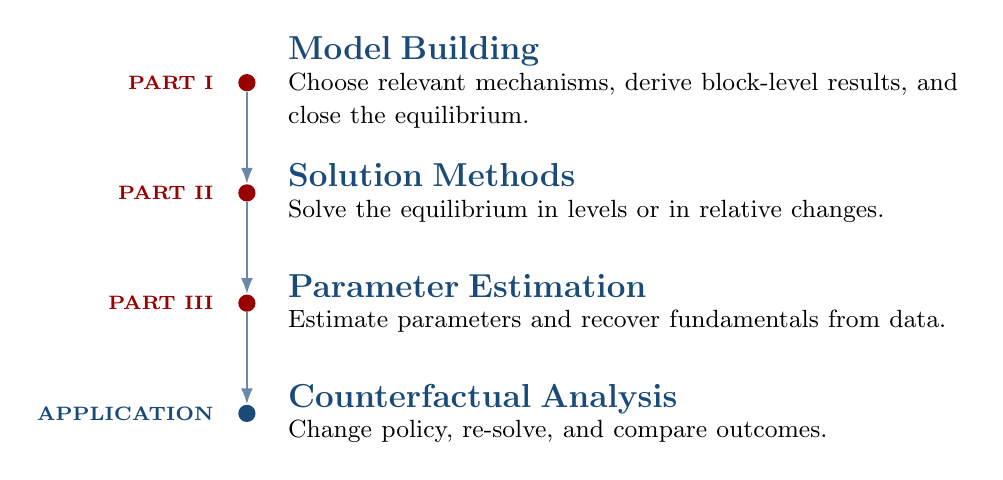
\begin{tikzpicture}[
    body/.style={anchor=west,align=left,text width=8.6cm},
    marker/.style={circle,fill=deepred,inner sep=2.2pt},
    flow/.style={-{Latex[length=2mm]},draw=blue1!65,line width=0.7pt}
  ]
    \node[marker] (m1) at (-4.25,0.55) {};
    \node[anchor=east,text=deepred,font=\scriptsize\bfseries] at (-4.55,0.55)
      {PART I};
    \node[body] at (-3.85,0.55) {
      {\large\B{Model Building}}\\[-1pt]
      {\small Choose relevant mechanisms, derive block-level results, and close the equilibrium.}
    };

    \node[marker] (m2) at (-4.25,-0.85) {};
    \node[anchor=east,text=deepred,font=\scriptsize\bfseries] at (-4.55,-0.85)
      {PART II};
    \node[body] at (-3.85,-0.85) {
      {\large\B{Solution Methods}}\\[-1pt]
      {\small Solve the equilibrium in levels or in relative changes.}
    };

    \node[marker] (m3) at (-4.25,-2.25) {};
    \node[anchor=east,text=deepred,font=\scriptsize\bfseries] at (-4.55,-2.25)
      {PART III};
    \node[body] at (-3.85,-2.25) {
      {\large\B{Parameter Estimation}}\\[-1pt]
      {\small Estimate parameters and recover fundamentals from data.}
    };

    \node[marker,fill=blue1] (m4) at (-4.25,-3.65) {};
    \node[anchor=east,text=blue1,font=\scriptsize\bfseries] at (-4.55,-3.65)
      {APPLICATION};
    \node[body] at (-3.85,-3.65) {
      {\large\B{Counterfactual Analysis}}\\[-1pt]
      {\small Change policy, re-solve, and compare outcomes.}
    };

    \draw[flow] (m1) -- (m2);
    \draw[flow] (m2) -- (m3);
    \draw[flow] (m3) -- (m4);
  \end{tikzpicture}
\end{frame}

\section{Part I: Model Building}

\partdivider{I}{Model Building}

\begin{frame}[t]{A Menu of Model Components}
  \small
  \begin{columns}[T,onlytextwidth]
    \column{0.49\textwidth}
      \B{Module 1: Preferences}\\[-2pt]
      {\footnotesize Goods, sectors, local factors, and preference heterogeneity.}

      \medskip
      \B{Module 2: Production Technology}\\[-2pt]
      {\footnotesize Returns to scale, productivity, input--output linkages, and local factors.}

      \medskip
      \B{Module 3: Commodity Trade}\\[-2pt]
      {\footnotesize Variable or fixed trade costs, asymmetry, geography, and nontraded goods.}

      \medskip
      \B{Module 4: Technology for Idea Flows}\\[-2pt]
      {\footnotesize Knowledge diffusion, innovation, and the transferability of ideas.}

    \column{0.47\textwidth}
      \B{Module 5: Migration}\\[-2pt]
      {\footnotesize Static or dynamic location choice, migration costs, and worker heterogeneity.}

      \medskip
      \B{Module 6: Endowments}\\[-2pt]
      {\footnotesize Population and skills, housing or land, capital, and infrastructure.}

      \medskip
      \B{Module 7: Equilibrium}\\[-2pt]
      {\footnotesize Goods-market clearing, labor-market clearing, and trade balance.}

      \medskip
      \B{The menu is open-ended}\\[-2pt]
      {\footnotesize Other institutions or frictions can be added when required by the question.}
  \end{columns}

  \vfill
  \centering
  \hi{A model selects one concrete specification from each relevant menu.}
\end{frame}

\begin{frame}[t]{The Model Used in This Lecture}
  \footnotesize
  \renewcommand{\arraystretch}{1.18}
  \begin{tabular}{
    >{\raggedright\arraybackslash}p{0.28\textwidth}
    >{\raggedright\arraybackslash}p{0.64\textwidth}}
    \toprule
    Menu & Baseline selection \\
    \midrule
    Preferences
      & CES consumption aggregator over a single sector of differentiated goods. \\
    Production technology
      & Labor-only technology with a fixed cost under monopolistic competition. \\
    Commodity trade
      & CES gravity with differentiated varieties and iceberg trade costs. \\
    Idea flows
      & None: location productivity is exogenous. \\
    Migration
      & Static discrete choice over indirect utility, including housing congestion
        and idiosyncratic preference shocks. \\
    Endowments
      & Homogeneous labor, fixed local housing stocks, fixed total population,
        and no mobile capital. \\
    Equilibrium
      & General equilibrium with goods-market clearing, labor-market clearing,
        and trade balance. \\
    \bottomrule
  \end{tabular}

  \vfill
  \centering
  \hi{The following slides derive selected blocks; the remaining choices stay explicit.}
\end{frame}

\subsection{Module 1: Preferences}

\begin{frame}{What does a household choose?}
  \small
  Consumers in location \(n\) allocate expenditure across varieties produced
  in origins \(i\in\mathcal N\). Each active firm supplies one variety, and
  \(M_i\) is the endogenous mass of active firms in origin \(i\):
  \[
    C_n=
    \left[
      \sum_{i\in\mathcal N}
      \int_0^{M_i}
      c_{ni}(j)^{\frac{\sigma-1}{\sigma}}\,dj
    \right]^{\frac{\sigma}{\sigma-1}},
    \qquad \sigma>1.
  \]
  Let \(E_n\) denote aggregate disposable income spent on differentiated
  consumption goods in location \(n\). The representative household allocates
  \(E_n\) across varieties:
  \[
    \max_{\{c_{ni}(j)\}} C_n
    \quad\text{s.t.}\quad
    \sum_{i\in\mathcal N}\int_0^{M_i}
      p_{ni}(j)c_{ni}(j)\,dj=E_n.
  \]
  \begin{itemize}
    \item one sector with horizontally differentiated varieties;
    \item \(M_i\) is the endogenous mass of firms---and therefore varieties---in origin \(i\);
    \item \(\sigma\) is the elasticity of substitution across goods;
  \end{itemize}
\end{frame}

\begin{frame}[t,label=mainPreferences]{Result: Demand and the Cost of Living}
  \small
  \setlength{\abovedisplayskip}{3pt}
  \setlength{\belowdisplayskip}{3pt}

  \begin{columns}[T,onlytextwidth]
    \column{0.53\textwidth}
      \B{Concrete equations}
    \column{0.43\textwidth}
      \B{General form}
  \end{columns}

  \smallskip
  \begin{columns}[T,onlytextwidth]
    \column{0.53\textwidth}
      \B{Demand}
      \[
        c_{ni}(j)
        =
        p_{ni}(j)^{-\sigma}P_n^{\sigma-1}E_n.
      \]
    \column{0.43\textwidth}
      \B{Demand}
      \[
        \mathbf c_n
        =\mathcal D_n(E_n,\mathbf p_n,P_n;\boldsymbol\phi),
      \]
  \end{columns}

  \smallskip
  \begin{columns}[T,onlytextwidth]
    \column{0.53\textwidth}
      \B{Price index}
      \[
        P_n
        =
        \left[
          \sum_{i\in\mathcal N}\int_0^{M_i}
            p_{ni}(j)^{1-\sigma}dj
         \right]^{1/(1-\sigma)}.
      \]
    \column{0.43\textwidth}
      \B{Price index}
      \[
        P_n
        =\mathcal P_n(\mathbf p_n,\mathbf M;\boldsymbol\phi).
      \]
  \end{columns}
  \smallskip
  {\footnotesize
  \(\boldsymbol\phi\) collects the exogenous parameters and fundamentals
  relevant to the module.}
  \smallskip
  \hfill\derivlink{appCES}
\end{frame}

\subsection{Module 2: Production Technology}

\begin{frame}{How Does a Firm Produce?}
  A firm in location \(i\) produces one differentiated variety \(j\):
  \[
    \ell_i(j)=F+\frac{x_i(j)}{A_i},
    \qquad F>0,\quad A_i>0.
  \]
  Shipping to \(n\) requires \(d_{ni}\geq1\) units at origin per unit delivered.
  Hence delivered marginal cost is
  \[
    mc_{ni}=d_{ni}\frac{w_i}{A_i}.
  \]
  \begin{itemize}
    \item \(A_i\): local labor productivity;
    \item \(w_i\): local factor price;
    \item \(F\): fixed labor requirement;
    \item \(d_{ni}\): bilateral iceberg trade friction.
  \end{itemize}
\end{frame}

\begin{frame}[t,label=mainProduction]{Result: Delivered Prices and Firm Mass}
  \small
  \setlength{\abovedisplayskip}{3pt}
  \setlength{\belowdisplayskip}{3pt}
  \B{Market structure:} monopolistic competition with CES demand and free entry.

  \smallskip
  \begin{columns}[T,onlytextwidth]
    \column{0.53\textwidth}
      \B{Concrete equations}
    \column{0.43\textwidth}
      \B{General form}
  \end{columns}

  \smallskip
  \begin{columns}[T,onlytextwidth]
    \column{0.53\textwidth}
      \B{Delivered price (profit maximization)}
      \[
        p_{ni}
        =
        \underbrace{\frac{\sigma}{\sigma-1}}_{\text{markup}}
        \underbrace{d_{ni}\frac{w_i}{A_i}}_{\text{delivered marginal cost}}.
      \]
    \column{0.43\textwidth}
      \B{Delivered price}
      \[
        \mathbf p_i
        =\mathcal C_i(w_i;\boldsymbol\phi),
      \]
  \end{columns}

  \smallskip
  \begin{columns}[T,onlytextwidth]
    \column{0.53\textwidth}
      \B{Mass of firms (local labor-market clearing)}
      \[
        M_i=\frac{L_i}{\sigma F}.
      \]
    \column{0.43\textwidth}
      \B{Mass of firms}
      \[
        M_i
        =\mathcal M_i(L_i;\boldsymbol\phi).
      \]
  \end{columns}
  \smallskip
  \hfill\derivlink{appProduction}

\end{frame}

\subsection{Module 3: Commodity Trade}

\begin{frame}[t,label=mainTradeShares]{Result: Trade Shares}
  \small
  CES demand and symmetry across firms imply
  \begin{columns}[T,onlytextwidth]
    \column{0.64\textwidth}
      \B{Concrete equation}

      \B{Trade share}
      \[
        \begin{aligned}
          \pi_{ni}
          &\equiv
          \frac{
            \displaystyle\int_0^{M_i}p_{ni}(j)c_{ni}(j)\,dj
          }{
            \displaystyle\sum_k\int_0^{M_k}p_{nk}(j)c_{nk}(j)\,dj
          }
          \\[3pt]
          &=
          \frac{M_ip_{ni}c_{ni}}
               {\sum_kM_kp_{nk}c_{nk}}
          \\[3pt]
          &=
          \frac{M_ip_{ni}^{1-\sigma}}
               {\sum_kM_kp_{nk}^{1-\sigma}}
          .
        \end{aligned}
      \]

    \column{0.31\textwidth}
      \B{General form}

      \B{Trade shares}
      \[
        \boldsymbol\pi_n
        =
        \mathcal X_n(\mathbf p_n,\mathbf M;\boldsymbol\phi).
      \]
  \end{columns}

  \smallskip
  \hfill\derivlink{appTrade}
\end{frame}

\subsection{Module 4: Technology for Idea Flows}

\begin{frame}{Choices for Idea Flows}
  \renewcommand{\arraystretch}{1.25}
  \begin{tabular}{
    >{\raggedright\arraybackslash}p{0.28\textwidth}
    >{\raggedright\arraybackslash}p{0.62\textwidth}}
    \toprule
    Choice & Economic content \\
    \midrule
    No idea flows
      & Local productivity is exogenous. \\
    Exogenous diffusion
      & Knowledge arriving from other locations shifts local productivity. \\
    Endogenous innovation and diffusion
      & Economic activity creates ideas and affects how they spread across space. \\
    \bottomrule
  \end{tabular}

  \vfill
  \B{Selection in this lecture: no idea flows}
  \[
    A_i=\bar A_i,
    \qquad i\in\mathcal N.
  \]
\end{frame}

\subsection{Module 5: Migration}

\begin{frame}{Static Discrete-Choice Migration}
  \small
  \setlength{\abovedisplayskip}{3pt}
  \setlength{\belowdisplayskip}{3pt}
  \B{Location payoff.}\quad Each worker \(o\) chooses a location. Conditional on \(n\),
  \[
    U_{no}
    =
    B_n
    \left(\frac{C_n}{\alpha}\right)^\alpha
    \left(\frac{h_n}{1-\alpha}\right)^{1-\alpha}
    z_{no},
    \qquad
    P_nC_n+r_nh_n
    =
    y_n+t_n.
  \]
  Housing rents are rebated lump-sum to local residents. The local housing
  stock \(H_n\) is fixed and the housing market clears, so
  \[
    t_n=\frac{r_nH_n}{L_n}=r_nh_n.
  \]

  \B{Idiosyncratic location preference.}
  \[
    \Pr(z_{no}\leq z)
    =
    \exp\!\left(-z^{-\kappa}\right),
    \qquad \kappa>1.
  \]
  {\scriptsize
  \(y_n=E_n/L_n\) is per-capita disposable income excluding housing rents;
  housing rents are rebated locally; \(B_n\) is the amenity;
  and \(\kappa\) is the mobility elasticity.}
\end{frame}

\begin{frame}[t,label=mainMigration]{Migration Shares}
  \small
  \begin{columns}[T,onlytextwidth]
    \column{0.64\textwidth}
      \B{Concrete equation}

      \B{Migration share}
      \[
        \lambda_n
        =
        \frac{
          \left[
          B_n\dfrac{y_n}
          {P_n^\alpha r_n^{1-\alpha}}
          \right]^\kappa
        }{
          \displaystyle\sum_k
          \left[
          B_k\dfrac{y_k}
          {P_k^\alpha r_k^{1-\alpha}}
          \right]^\kappa
        }.
      \]

    \column{0.31\textwidth}
      \B{General form}

      \B{Migration share}
      \[
        \boldsymbol\lambda
        =
        \mathcal S(\mathbf y,\mathbf P,\mathbf r;
        \boldsymbol\phi).
      \]
  \end{columns}

  The Cobb--Douglas normalization cancels from location shares. This block
  leaves \(r_n\) as an equilibrium price; Module 7 imposes housing-market clearing.

  \smallskip
  \hfill\derivlink{appHousingIncome}
\end{frame}

\subsection{Module 6: Endowments}

\begin{frame}[t]{What Is Taken as Given?}
  \begin{columns}[T,onlytextwidth]
    \column{0.47\textwidth}
      \B{Choices on the menu}
      \begin{itemize}\setlength{\itemsep}{5pt}
        \item population and worker skills;
        \item housing or land endowments;
        \item spatial scope and geographic units;
        \item capital and infrastructure.
      \end{itemize}

    \column{0.47\textwidth}
      \B{Baseline selection}
      \begin{itemize}\setlength{\itemsep}{5pt}
        \item homogeneous workers;
        \item a fixed set of locations $\mathcal N$;
        \item fixed local housing stocks \(\{H_i\}_{i\in\mathcal N}\);
        \item fixed aggregate labor $\bar L$;
        \item no mobile capital stock;
        \item infrastructure represented through trade costs $d_{ni}$.
      \end{itemize}
  \end{columns}
\end{frame}

\subsection{Module 7: Equilibrium}

\begin{frame}[t,label=mainEquilibrium]{Four Equilibrium Conditions}
  \small
  \setlength{\abovedisplayskip}{2pt}
  \setlength{\belowdisplayskip}{2pt}
  \setlength{\abovedisplayshortskip}{2pt}
  \setlength{\belowdisplayshortskip}{2pt}

  \begin{columns}[T,onlytextwidth]
    \column{0.55\textwidth}
      \B{Concrete equations}
    \column{0.40\textwidth}
      \B{General form}
  \end{columns}

  \smallskip
  \begin{columns}[T,onlytextwidth]
    \column{0.55\textwidth}
      \B{Goods-market clearing}
      \[
        w_iL_i=\sum_n\pi_{ni}E_n.
      \]
    \column{0.40\textwidth}
      \B{Goods-market clearing}
      \[
        \mathbf w
        =\mathcal W(\boldsymbol\pi,\mathbf E,\mathbf L;\boldsymbol\phi).
      \]
  \end{columns}

  \smallskip
  \begin{columns}[T,onlytextwidth]
    \column{0.55\textwidth}
      \B{Labor-market clearing}
      \[
        L_i=\bar L\lambda_i.
      \]
    \column{0.40\textwidth}
      \B{Labor-market clearing}
      \[
        \mathbf L
        =\mathcal L(\boldsymbol\lambda;\boldsymbol\phi).
      \]
  \end{columns}

  \medskip
  \begin{columns}[T,onlytextwidth]
    \column{0.55\textwidth}
      \B{Housing-market clearing}
      \[
        H_i=L_ih_i
        \quad\Longrightarrow\quad
        r_i=\frac{1-\alpha}{\alpha}\frac{y_iL_i}{H_i}.
      \]
    \column{0.40\textwidth}
      \B{Housing-market clearing}
      \[
        \mathbf r
        =\mathcal R(\mathbf y,\mathbf L;\boldsymbol\phi).
      \]
  \end{columns}

  \medskip
  \begin{columns}[T,onlytextwidth]
    \column{0.55\textwidth}
      \B{Trade balance}
      \[
        \begin{aligned}
          IM_i&=(1-\pi_{ii})E_i,\\
          EX_i&=w_iL_i-\pi_{ii}E_i,\\
          IM_i&=EX_i+D_i
            \quad\Longrightarrow\quad E_i=w_iL_i+D_i.
        \end{aligned}
      \]
      {\footnotesize \(D_i\) is an exogenous trade deficit.}
    \column{0.40\textwidth}
      \B{Trade balance}
      \[
        \mathbf E
        =\mathcal E(\mathbf w,\mathbf L;\boldsymbol\phi).
      \]
  \end{columns}

  \vfill
  \hfill\derivlink{appEquilibrium}
\end{frame}

\begin{frame}[t]{Assembling the Model}
  \scriptsize
  \B{Unknown vector (11 blocks with 11 unknown matrices):}\quad
  \(\mathbf z=(\mathbf c,\mathbf p,\mathbf P,\mathbf M,
  \boldsymbol\pi,\boldsymbol\lambda,\mathbf w,\mathbf L,\mathbf E,
  \mathbf y,\mathbf r)\).

  \vspace{-0.15em}
  {
  \renewcommand{\arraystretch}{0.78}
  \begin{tabular}{
    @{}>{\raggedright\arraybackslash}m{0.24\textwidth}
    >{\centering\arraybackslash}m{0.39\textwidth}
    >{\centering\arraybackslash}m{0.31\textwidth}@{}}
    & \B{Concrete equation} & \B{General form} \tabularnewline[0.08em]

    \mbox{\B{Demand}}
      & \(\displaystyle c_{ni}=p_{ni}^{-\sigma}P_n^{\sigma-1}E_n\)
      & \(\displaystyle \mathbf c=\mathcal D(\mathbf E,\mathbf p,\mathbf P;\boldsymbol\phi)\)
      \tabularnewline[0.12em]

    \mbox{\B{Price index}}
      & \(\displaystyle P_n=\left[\sum_iM_ip_{ni}^{1-\sigma}\right]^{1/(1-\sigma)}\)
      & \(\displaystyle \mathbf P=\mathcal P(\mathbf p,\mathbf M;\boldsymbol\phi)\)
      \tabularnewline[0.24em]

    \mbox{\B{Delivered price}}
      & \(\displaystyle p_{ni}=\mu d_{ni}w_i/A_i\)
      & \(\displaystyle \mathbf p=\mathcal C(\mathbf w;\boldsymbol\phi)\)
      \tabularnewline[0.12em]

    \mbox{\B{Firm mass}}
      & \(\displaystyle M_i=L_i/(\sigma F)\)
      & \(\displaystyle \mathbf M=\mathcal M(\mathbf L;\boldsymbol\phi)\)
      \tabularnewline[0.14em]

    \mbox{\B{Trade share}}
      & \(\displaystyle \pi_{ni}=\frac{M_ip_{ni}^{1-\sigma}}
        {\sum_kM_kp_{nk}^{1-\sigma}}\)
      & \(\displaystyle \boldsymbol\pi=\mathcal T(\mathbf p,\mathbf M;\boldsymbol\phi)\)
      \tabularnewline[0.30em]

    \mbox{\B{Migration share}}
      & \(\displaystyle
        \lambda_n=
        \frac{\left[
        B_ny_n/(P_n^\alpha r_n^{1-\alpha})\right]^\kappa}
        {\sum_k\left[
        B_ky_k/(P_k^\alpha r_k^{1-\alpha})\right]^\kappa}\)
      & \(\displaystyle \boldsymbol\lambda=\mathcal S
        (\mathbf y,\mathbf P,\mathbf r;\boldsymbol\phi)\)
      \tabularnewline[0.26em]

    \mbox{\B{Disposable income}}
      & \(\displaystyle y_i=\frac{E_i}{L_i}\)
      & \(\displaystyle \mathbf y=\mathcal Y
        (\mathbf E,\mathbf L;\boldsymbol\phi)\)
      \tabularnewline[0.12em]

    \mbox{\B{Housing rent}}
      & \(\displaystyle r_i=\frac{1-\alpha}{\alpha}\frac{y_iL_i}{H_i}\)
      & \(\displaystyle \mathbf r=\mathcal R
        (\mathbf y,\mathbf L;\boldsymbol\phi)\)
      \tabularnewline[0.12em]

    \mbox{\B{Goods-market clearing}}
      & \(\displaystyle w_iL_i=\sum_n\pi_{ni}E_n\)
      & \(\displaystyle \mathbf w=\mathcal W(\boldsymbol\pi,\mathbf E,\mathbf L;\boldsymbol\phi)\)
      \tabularnewline[0.14em]

    \mbox{\B{Labor-market clearing}}
      & \(\displaystyle L_i=\bar L\lambda_i\)
      & \(\displaystyle \mathbf L=\mathcal L(\boldsymbol\lambda;\boldsymbol\phi)\)
      \tabularnewline[0.14em]

    \mbox{\B{Trade balance}}
      & \(\displaystyle E_i=w_iL_i+D_i\)
      & \(\displaystyle \mathbf E=\mathcal E
        (\mathbf w,\mathbf L;\boldsymbol\phi)\)
      \tabularnewline
  \end{tabular}
  }
\end{frame}

\begin{frame}[t]{Reducing the Model to Five Equation Blocks}
  \scriptsize
  \B{Given}\quad
  fundamentals \(\{A_i,B_i,H_i\}_i\), trade frictions
  \(\{d_{ni}\}_{n,i}\), parameters \((\alpha,F,\sigma,\kappa)\),
  total labor \(\bar L\), and balanced trade \(\mathbf D=\mathbf0\).

  \smallskip
  \B{Solve for}\quad
  \(\{\mathbf P,\boldsymbol\pi,\mathbf w,
  \boldsymbol\lambda,\mathbf L\}\), with
  \(\mu=\sigma/(\sigma-1)\).

  \vspace{0.3em}
  {
  \renewcommand{\arraystretch}{0.98}
  \begin{tabular}{
    @{}>{\raggedright\arraybackslash}m{0.25\textwidth}
    >{\centering\arraybackslash}m{0.46\textwidth}
    >{\centering\arraybackslash}m{0.23\textwidth}@{}}
    & \B{Concrete equation} & \B{General form} \tabularnewline[0.45em]

    \mbox{\B{Price index}}
      & \(\displaystyle
        P_n=\mu\left[
          \frac{1}{\sigma F}\sum_iL_i
          \left(d_{ni}\frac{w_i}{A_i}\right)^{1-\sigma}
        \right]^{\frac{1}{1-\sigma}}
        \)
      & \(\displaystyle \mathbf P=\mathcal P(\mathbf w,\mathbf L;\boldsymbol\phi)\)
      \tabularnewline[0.60em]

    \mbox{\B{Trade share}}
      & \(\displaystyle
        \pi_{ni}=\frac{L_i(d_{ni}w_i/A_i)^{1-\sigma}}
        {\sum_kL_k(d_{nk}w_k/A_k)^{1-\sigma}}
        \)
      & \(\displaystyle \boldsymbol\pi=\mathcal T(\mathbf w,\mathbf L;\boldsymbol\phi)\)
      \tabularnewline[0.60em]

    \mbox{\B{Goods-market clearing}}
      & \(\displaystyle
        w_iL_i=\sum_n\pi_{ni}w_nL_n
        \)
      & \(\displaystyle \mathbf w=\mathcal W(\boldsymbol\pi,\mathbf L;\boldsymbol\phi)\)
      \tabularnewline[0.60em]

    \mbox{\B{Migration share}}
      & \(\displaystyle
        \lambda_n=\frac{
          \left[
          B_n\frac{w_n^\alpha H_n^{1-\alpha}}
          {P_n^\alpha L_n^{1-\alpha}}
          \right]^\kappa
        }{
          \displaystyle\sum_k\left[
          B_k\frac{w_k^\alpha H_k^{1-\alpha}}
          {P_k^\alpha L_k^{1-\alpha}}
          \right]^\kappa
        }
        \)
      & \(\displaystyle \boldsymbol\lambda=\mathcal S
        (\mathbf w,\mathbf P,\mathbf L;\boldsymbol\phi)\)
      \tabularnewline[0.60em]

    \mbox{\B{Labor-market clearing}}
      & \(\displaystyle L_n=\bar L\lambda_n\)
      & \(\displaystyle \mathbf L=\mathcal L
        (\boldsymbol\lambda;\boldsymbol\phi)\)
      \tabularnewline
  \end{tabular}
  }

  \vspace{-0.1em}
  \B{Fixed-point representation}\quad
  After substituting out \(\mathbf P\), \(\boldsymbol\pi\), and
  \(\boldsymbol\lambda\), define
  \[
    \mathbf x\equiv(\mathbf w,\mathbf L),
    \qquad
    \mathbf x=\mathcal F(\mathbf x;\boldsymbol\phi).
  \]
\end{frame}

\section{Part II: Solution Methods}

\partdivider{II}{Solution Methods}

\subsection{Method 1: Levels Solution}

\begin{frame}{Fixed-Point Iteration}
  \small
  Let \(k=0,1,2,\ldots\) denote the iteration counter.
  \begin{enumerate}\setlength{\itemsep}{5pt}
    \item \B{Guess.} Choose initial \(\{w_i^{(0)}\}\) and
      \(\{L_i^{(0)}\}\); use
      \(\operatorname{geomean}_{i\in\mathrm{West}}w_i=1\) as the wage
      numeraire.
    \item \B{Price index (at \(k\)).} Given \((\mathbf w^{(k)},\mathbf L^{(k)})\),
      compute \(\mathbf P^{(k)}\).
    \item \B{Shares (at \(k\)).} Compute \(\boldsymbol\pi^{(k)}\) and
      \(\boldsymbol\lambda^{(k)}\).
    \item \B{Implied new values (\(k+1\)).} Update
      \[
        L_n^{(k+1)}=\bar L\lambda_n^{(k)},
        \qquad
        w_i^{(k+1)}
        =\frac{1}{L_i^{(k)}}
          \sum_n w_n^{(k)}L_n^{(k)}\pi_{ni}^{(k)}.
      \]
    \item \B{Compare.} If \((\mathbf w^{(k+1)},\mathbf L^{(k+1)})\) is
      close to \((\mathbf w^{(k)},\mathbf L^{(k)})\), stop.
    \item \B{Update.} Otherwise set \(k\leftarrow k+1\) and return to step 2.
  \end{enumerate}
\end{frame}

\subsection{Method 2: Exact-Hat Algebra}

\begin{frame}{The High-Dimensionality Problem}
  A level solution requires fundamentals, parameters, and endowments:
  \[
    \underbrace{\{A_i,B_i,H_i\}_{i=1}^{N}}_{3N\text{ location fundamentals}},
    \qquad
    \underbrace{\{d_{ni}\}_{n,i=1}^{N}}_{N^2\text{ bilateral trade costs}}.
  \]
  \[
    \underbrace{\alpha,\sigma,\kappa,F,\{\bar L_c\}_c}
      _{\text{common parameters and country labor endowments}}.
  \]
  With \(N=100\), bilateral trade costs alone contain \(10{,}000\) elements.

  \medskip
  Many of these level fundamentals are unobserved. Recovering every
  \(A_i,B_i,H_i\), and \(d_{ni}\) is therefore empirically demanding.
  In contrast, the baseline equilibrium supplies observable outcomes such as
  \[
    \mathbf b=\{\mathbf w,\mathbf L,\boldsymbol\pi,\boldsymbol\lambda\},
    \qquad
    \pi_{ni}=\frac{X_{ni}}{\sum_kX_{nk}}.
  \]

  \vfill
  \B{Question:}\quad Can we conduct counterfactual policy analysis using the
  observed baseline equilibrium, without recovering every high-dimensional
  level fundamental?
\end{frame}

\begin{frame}{What Exact-Hat Algebra Does}
  Counterfactual analysis usually asks how equilibrium outcomes change after a
  policy shock. For any object \(x\), define
  \[
    \wh x\equiv\frac{x'}{x},
  \]
  where \(x\) is the baseline level and \(x'\) is the counterfactual level.

  Exact-hat algebra rewrites the equilibrium in proportional changes using
  \[
    \underbrace{\{\mathbf w,\mathbf L,\boldsymbol\pi,
      \boldsymbol\lambda\}}_{\text{observed baseline}}
    +\underbrace{(\alpha,\sigma,\kappa)}_{\text{structural parameters}}
    +\underbrace{\{\wh A,\wh d,\wh B,\wh H,
      \wh F,\wh{\bar L}\}}_{\text{shocks}}.
  \]

  \B{Result:}\quad solve directly for \(\{\wh{\mathbf w},\wh{\mathbf L}\}\).
  The high-dimensional levels \(\{A_i,d_{ni},B_i,H_i\}\) no longer need to be
  recovered separately; baseline shares become the weights in the hat system.
\end{frame}

\begin{frame}[t,label=mainHatSystem]{Exact-Hat System}
  \scriptsize
  \B{Given}\quad
  \(\mathbf b\equiv\{\mathbf w,\mathbf L,\boldsymbol\pi,
  \boldsymbol\lambda\}\) (baseline observables),
  \(\boldsymbol\theta\equiv(\alpha,\sigma,\kappa)\) (structural parameters), and
  \(\wh{\mathbf s}\equiv\{\wh A,\wh d,\wh B,\wh H,\wh F,
  \wh{\bar L}\}\) (shocks).
  \qquad
  \B{Solve for}\quad \(\{\wh{\mathbf P},\wh{\boldsymbol\pi},
  \wh{\mathbf w},\wh{\boldsymbol\lambda},\wh{\mathbf L}\}\).

  \vspace{0.35em}
  {
  \renewcommand{\arraystretch}{0.98}
  \begin{tabular}{
    @{}>{\raggedright\arraybackslash}m{0.25\textwidth}
    >{\centering\arraybackslash}m{0.45\textwidth}
    >{\centering\arraybackslash\fontsize{7}{8}\selectfont}m{0.24\textwidth}@{}}
    & \B{Concrete equation} & \B{General form} \tabularnewline[0.35em]

    \mbox{\B{Price index}\,\hyperlink{deriveHatPrice}{\textcolor{blue1}{\(\rightarrow\)}}}
      & \(\displaystyle
        \wh P_n^{1-\sigma}
        =\wh F^{-1}\sum_i\pi_{ni}\wh L_i
        \left(\frac{\wh d_{ni}\wh w_i}{\wh A_i}\right)^{1-\sigma}
        \)
      & \(\displaystyle
        \wh{\mathbf P}=\widehat{\mathcal P}_{\wh{\mathbf s}}
        (\wh{\mathbf w},\wh{\mathbf L};\mathbf b,\boldsymbol\theta)\)
      \tabularnewline[0.45em]

    \mbox{\B{Trade share}\,\hyperlink{deriveHatTrade}{\textcolor{blue1}{\(\rightarrow\)}}}
      & \(\displaystyle
        \wh\pi_{ni}
        =\frac{\wh F^{-1}\wh L_i
        (\wh d_{ni}\wh w_i/\wh A_i)^{1-\sigma}}
        {\wh P_n^{1-\sigma}}
        \)
      & \(\displaystyle
        \wh{\boldsymbol\pi}=\widehat{\mathcal T}_{\wh{\mathbf s}}
        (\wh{\mathbf w},\wh{\mathbf L},\wh{\mathbf P};
        \mathbf b,\boldsymbol\theta)\)
      \tabularnewline[0.45em]

    \mbox{\B{Goods-market clearing}\,\hyperlink{deriveHatWage}{\textcolor{blue1}{\(\rightarrow\)}}}
      & \(\displaystyle
        \wh w_i
        =\frac{1}{\wh L_iw_iL_i}
        \sum_n\wh\pi_{ni}\wh w_n\wh L_n
        (w_nL_n\pi_{ni})
        \)
      & \(\displaystyle
        \wh{\mathbf w}=\widehat{\mathcal W}_{\wh{\mathbf s}}
        (\wh{\boldsymbol\pi},\wh{\mathbf w},\wh{\mathbf L};
        \mathbf b,\boldsymbol\theta)\)
      \tabularnewline[0.45em]

    \mbox{\B{Population share}\,\hyperlink{deriveHatMigration}{\textcolor{blue1}{\(\rightarrow\)}}}
      & \(\displaystyle
        \wh\lambda_n
        =\frac{\left[\wh B_n
        \frac{\wh w_n^\alpha\wh H_n^{1-\alpha}}
        {\wh P_n^\alpha\wh L_n^{1-\alpha}}\right]^\kappa}
        {\sum_{k\in c}\lambda_k
        \left[\wh B_k
        \frac{\wh w_k^\alpha\wh H_k^{1-\alpha}}
        {\wh P_k^\alpha\wh L_k^{1-\alpha}}\right]^\kappa}
        \)
      & \(\displaystyle
        \wh{\boldsymbol\lambda}=\widehat{\mathcal S}_{\wh{\mathbf s}}
        (\wh{\mathbf w},\wh{\mathbf P},\wh{\mathbf L};
        \mathbf b,\boldsymbol\theta)\)
      \tabularnewline[0.45em]

    \mbox{\B{Labor-market clearing}\,\hyperlink{deriveHatMigration}{\textcolor{blue1}{\(\rightarrow\)}}}
      & \(\displaystyle
        \wh L_n=\wh{\bar L}\,\wh\lambda_n
        \)
      & \(\displaystyle
        \wh{\mathbf L}=\widehat{\mathcal L}_{\wh{\mathbf s}}
        (\wh{\boldsymbol\lambda};\mathbf b,\boldsymbol\theta)\)
      \tabularnewline
  \end{tabular}
  }

  \vfill
  \B{Fixed-point form}\quad
  \(\wh{\mathbf x}\equiv(\wh{\mathbf w},\wh{\mathbf L})\),
  \qquad
  \(\wh{\mathbf x}
    =\widehat{\mathcal F}_{\wh{\mathbf s}}
    (\wh{\mathbf x};\mathbf b,\boldsymbol\theta)\),
  \[
    \mathbf b\equiv
      \{\mathbf w,\mathbf L,\boldsymbol\pi,\boldsymbol\lambda\}
      \ \text{(baseline observables)},
    \qquad
    \boldsymbol\theta\equiv(\alpha,\sigma,\kappa)
      \ \text{(structural parameters)}.
  \]
\end{frame}

\begin{frame}[t,label=deriveHatPrice]{Derivation 1: Price-Index Hat}
  \footnotesize
  \B{Step 1. Start from the baseline and counterfactual price indices.}
  \[
    P_n^{1-\sigma}
      =\frac{\mu^{1-\sigma}}{\sigma F}
        \sum_iL_i\left(d_{ni}\frac{w_i}{A_i}\right)^{1-\sigma},
    \qquad
    P_n'^{\,1-\sigma}
      =\frac{\mu^{1-\sigma}}{\sigma F'}
        \sum_iL_i'\left(d_{ni}'\frac{w_i'}{A_i'}\right)^{1-\sigma}.
  \]

  \B{Step 2. Take the ratio; the common markup term cancels.}
  \[
    \frac{P_n'^{\,1-\sigma}}{P_n^{1-\sigma}}
    =\wh F^{-1}
      \frac{\sum_iL_i'
        (d_{ni}'w_i'/A_i')^{1-\sigma}}
           {\sum_kL_k(d_{nk}w_k/A_k)^{1-\sigma}}.
  \]

  \B{Step 3. Substitute hats and recognize the baseline trade share.}
  \[
    \wh P_n^{1-\sigma}
    =\wh F^{-1}\sum_i
      \underbrace{\frac{L_i(d_{ni}w_i/A_i)^{1-\sigma}}
      {\sum_kL_k(d_{nk}w_k/A_k)^{1-\sigma}}}_{\displaystyle \pi_{ni}}
      \wh L_i
      \left(\frac{\wh d_{ni}\wh w_i}{\wh A_i}\right)^{1-\sigma}.
  \]

  \vfill
  \hfill\backlink{mainHatSystem}{Back to Exact-Hat System}
\end{frame}

\begin{frame}[t,label=deriveHatTrade]{Derivation 2: Trade-Share Hat}
  \scriptsize
  \setlength{\abovedisplayskip}{3pt}
  \setlength{\belowdisplayskip}{3pt}
  \B{Step 1. Write the baseline and counterfactual trade shares.}
  \[
    \pi_{ni}
      =\frac{L_i(d_{ni}w_i/A_i)^{1-\sigma}}
      {\sum_kL_k(d_{nk}w_k/A_k)^{1-\sigma}},
    \qquad
    \pi_{ni}'
      =\frac{L_i'(d_{ni}'w_i'/A_i')^{1-\sigma}}
      {\sum_kL_k'(d_{nk}'w_k'/A_k')^{1-\sigma}}.
  \]

  \B{Step 2. Take the ratio and substitute primed objects with hats.}
  \[
    \wh\pi_{ni}
    =\frac{\wh L_i(\wh d_{ni}\wh w_i/\wh A_i)^{1-\sigma}}
      {\sum_k\pi_{nk}\wh L_k
      (\wh d_{nk}\wh w_k/\wh A_k)^{1-\sigma}}.
  \]

  \B{Step 3. Use the price-index hat to replace the denominator.}
  \[
    \wh P_n^{1-\sigma}
      =\wh F^{-1}\sum_k\pi_{nk}\wh L_k
      (\wh d_{nk}\wh w_k/\wh A_k)^{1-\sigma}
    \quad\Longrightarrow\quad
    \wh\pi_{ni}
    =\frac{\wh F^{-1}\wh L_i
      (\wh d_{ni}\wh w_i/\wh A_i)^{1-\sigma}}
      {\wh P_n^{1-\sigma}}.
  \]

  The levels \(A_i\) and \(d_{ni}\) disappear; their proportional shocks remain,
  while the observed baseline share \(\pi_{ni}\) supplies the weights.

  \vfill
  \hfill\backlink{mainHatSystem}{Back to Exact-Hat System}
\end{frame}

\begin{frame}[t,label=deriveHatMigration]{Derivation 3: Migration-Share Hat}
  \footnotesize
  \B{Step 1. Take the hat of within-location utility.}
  \[
    V_n=
      \frac{w_n^\alpha H_n^{1-\alpha}}
      {\alpha^\alpha(1-\alpha)^{1-\alpha}
      P_n^\alpha L_n^{1-\alpha}}
    \quad\Longrightarrow\quad
    \wh V_n
      =
      \frac{\wh w_n^\alpha\wh H_n^{1-\alpha}}
      {\wh P_n^\alpha\wh L_n^{1-\alpha}}.
  \]

  \B{Step 2. Write location shares in both equilibria.}
  \[
    \lambda_n=\frac{(B_nV_n)^\kappa}
      {\sum_{k\in c}(B_kV_k)^\kappa},
    \qquad
    \lambda_n'=\frac{(B_n'V_n')^\kappa}
      {\sum_{k\in c}(B_k'V_k')^\kappa}.
  \]

  \B{Step 3. Divide and use baseline shares as weights.}
  \[
    \wh\lambda_n
    =\frac{(\wh B_n\wh V_n)^\kappa}
      {\sum_{k\in c}\lambda_k
      (\wh B_k\wh V_k)^\kappa}.
  \]

  \B{Step 4. Take hats of labor-market clearing.}
  \[
    L_n=\bar L\lambda_n,
    \qquad
    L_n'=\bar L'\lambda_n'
    \quad\Longrightarrow\quad
    \wh L_n=\wh{\bar L}\,\wh\lambda_n.
  \]

  The levels \(B_n,H_n\) disappear; only their shocks remain, while the
  baseline population share \(\lambda_n\) becomes the weight.

  \vfill
  \hfill\backlink{mainHatSystem}{Back to Exact-Hat System}
\end{frame}

\begin{frame}[t,label=deriveHatWage]{Derivation 4: Wage Hat}
  \footnotesize
  \B{Step 1. Write goods-market clearing in both equilibria.}
  \[
    w_iL_i=\sum_nw_nL_n\pi_{ni},
    \qquad
    w_i'L_i'=\sum_nw_n'L_n'\pi_{ni}'.
  \]

  \B{Step 2. Replace counterfactual levels by baseline levels times hats.}
  \[
    \wh w_i\wh L_i(w_iL_i)
    =\sum_n\wh\pi_{ni}\wh w_n\wh L_n
      \underbrace{(w_nL_n\pi_{ni})}_{\text{baseline bilateral expenditure}}.
  \]

  \B{Step 3. Solve for the wage change.}
  \[
    \wh w_i
    =\frac{1}{\wh L_iw_iL_i}
      \sum_n\wh\pi_{ni}\wh w_n\wh L_n
      (w_nL_n\pi_{ni}).
  \]

  The equilibrium update uses baseline income and trade flows; it does not require
  separate recovery of \(A_i\) or \(d_{ni}\).

  \vfill
  \hfill\backlink{mainHatSystem}{Back to Exact-Hat System}
\end{frame}

\begin{frame}[t]{A 10\% U.S. Tariff on China}
  \footnotesize
  \B{Shock.}\quad Suppose the tariff applies to U.S. imports from China:
  \[
    \wh d_{\mathrm{US,CN}}
      \equiv\frac{1+t'_{\mathrm{US,CN}}}{1+t_{\mathrm{US,CN}}}=1.10,
    \qquad \wh d_{ni}=1\ \text{otherwise},
    \qquad
    \wh A_i=\wh B_i=\wh H_i=\wh F=\wh{\bar L}=1.
  \]

  \vspace{-0.4em}
  \begin{columns}[T,onlytextwidth]
    \begin{column}{0.61\textwidth}
      \B{The counterfactual system becomes}
      \begin{align*}
        \wh P_n^{1-\sigma}
          &=\sum_i\pi_{ni}\wh L_i
            (\wh d_{ni}\wh w_i)^{1-\sigma},\\
        \wh\pi_{ni}
          &=\frac{\wh L_i(\wh d_{ni}\wh w_i)^{1-\sigma}}
            {\wh P_n^{1-\sigma}},\\
        \wh w_i
          &=\frac{1}{\wh L_iw_iL_i}
            \sum_n\wh\pi_{ni}\wh w_n\wh L_n
            (w_nL_n\pi_{ni}),\\
        \wh\lambda_n
          &=\frac{\left[
            \wh w_n^\alpha/
            (\wh P_n^\alpha\wh L_n^{1-\alpha})
            \right]^\kappa}
            {\sum_{k\in c}\lambda_k\left[
            \wh w_k^\alpha/
            (\wh P_k^\alpha\wh L_k^{1-\alpha})
            \right]^\kappa},\\
        \wh L_n&=\wh\lambda_n.
      \end{align*}
    \end{column}
    \begin{column}{0.36\textwidth}
      \B{What must be supplied?}
      \begin{itemize}\setlength{\itemsep}{3pt}
        \item baseline bilateral expenditure shares \(\pi_{ni}\);
        \item baseline income and population \((w_iL_i,L_i)\);
        \item baseline population shares \(\lambda_i\);
        \item structural parameters \((\alpha,\sigma,\kappa)\);
        \item the tariff change \(\wh d_{\mathrm{US,CN}}\).
      \end{itemize}

      \medskip
      \B{What is not required?}\par
      The levels of \(A_i,d_{ni},B_i,H_i\), or \(P_i\).
    \end{column}
  \end{columns}

  \vfill
  \B{Exact-hat advantage:}\quad unchanged primitive hats equal one and disappear.
\end{frame}

\begin{frame}[t]{Counterfactual Iteration}
  \small
  \setlength{\abovedisplayskip}{2pt}
  \setlength{\belowdisplayskip}{2pt}
  Let \(k=0,1,2,\ldots\) denote the iteration counter.
  \begin{enumerate}\setlength{\itemsep}{2pt}\setlength{\parskip}{0pt}
    \item \B{Guess.}\quad \(\wh w_i^{(0)}=\wh L_i^{(0)}=1\); impose
      \(\operatorname{geomean}_{i\in\mathrm{West}}\wh w_i=1\).

    \item \B{Price index.}\quad Compute \(\wh P_n^{(k)}\) from
      \((\wh{\mathbf w}^{(k)},\wh{\mathbf L}^{(k)})\).

    \item \B{Shares.}\quad Compute \(\wh\pi_{ni}^{(k)}\) and
      \(\wh\lambda_n^{(k)}\).

    \item \B{Implied values.}\quad Compute
    \[
      \wh L_n^{(k+1)}=\wh{\bar L}\wh\lambda_n^{(k)},
      \qquad
      \wh w_i^{(k+1)}
      =\frac{\sum_n\wh\pi_{ni}^{(k)}\wh w_n^{(k)}\wh L_n^{(k)}
        (w_nL_n\pi_{ni})}
        {\wh L_i^{(k)}w_iL_i}.
    \]

    \item \B{Compare.}\quad Stop if the new wage and population hats are
      sufficiently close to their previous values.

    \item \B{Update.}\quad Otherwise damp the implied values:
    \[
      \wh w_i^{(k+1)}\leftarrow
        (1-\theta)\wh w_i^{(k)}+\theta\wh w_i^{(k+1)},
      \qquad
      \wh L_n^{(k+1)}\leftarrow
        (1-\theta)\wh L_n^{(k)}+\theta\wh L_n^{(k+1)},
      \quad \theta\in(0,1].
    \]
    Set \(k\leftarrow k+1\) and return to step 2.
  \end{enumerate}
\end{frame}

\section{Part III: Parameter Estimation}

\partdivider{III}{Parameter Estimation}

\setcounter{subsection}{0}

\subsection{Parameters and Fundamentals}

\begin{frame}[t]{Why Does Exact-Hat Algebra Help?}
  \small
  \B{The model in levels}
  \[
    \mathbf x\equiv(\mathbf w,\mathbf L),
    \qquad
    \mathbf x=\mathcal F(\mathbf x;\boldsymbol\phi),
  \]
  with
  \[
    \boldsymbol\phi
    =\Bigl(
      \underbrace{\{A_i,B_i,H_i\}_{i=1}^{N}}_{\text{location fundamentals}},
      \underbrace{\{d_{ni}\}_{n,i=1}^{N}}_{\text{bilateral trade costs}},
      \underbrace{\alpha,F,\sigma,\kappa,\{\bar L_c\}_c}
        _{\text{common parameters and country labor endowments}}
    \Bigr).
  \]
  Recovering all elements of \(\boldsymbol\phi\) is demanding: many location
  fundamentals are unobserved, while bilateral trade costs contain \(N^2\)
  elements.

  \smallskip
  \B{The same counterfactual in changes}
  \[
    \wh{\mathbf x}\equiv(\wh{\mathbf w},\wh{\mathbf L}),
    \qquad
    \wh{\mathbf x}
      =\widehat{\mathcal F}_{\wh{\mathbf s}}
        (\wh{\mathbf x};\mathbf b,\boldsymbol\theta),
  \]
  where
  \[
    \underbrace{\mathbf b
      =\{\mathbf w,\mathbf L,\boldsymbol\pi,\boldsymbol\lambda\}}
      _{\text{observed baseline equilibrium}},
    \qquad
    \underbrace{\boldsymbol\theta=(\alpha,\sigma,\kappa)}
      _{\text{structural parameters}}.
  \]

  \vfill
  \hi{Baseline observables replace the high-dimensional level fundamentals;
  only a small set of structural parameters still has to be estimated or calibrated.}
\end{frame}

\begin{frame}[t]{Structural Estimation: A Common Framework}
  \footnotesize
  Structural estimation chooses parameters to minimize the distance between
  the model and the data:
  \[
    \widehat{\boldsymbol\Theta}
      =
      \arg\min_{\boldsymbol\Theta\in\widetilde{\boldsymbol\Theta}}
      \widehat\Omega(\boldsymbol\Theta).
  \]
  The key choice is how to define the model--data distance
  \(\widehat\Omega(\boldsymbol\Theta)\).

  \smallskip
  \begin{columns}[T,onlytextwidth]
    \column{0.31\textwidth}
      \B{Model inversion}
      \[
        g^{\mathrm{model}}(\boldsymbol\Theta)
        =
        g^{\mathrm{data}}.
      \]
      Solve model equations directly for parameters or latent fundamentals.

    \column{0.31\textwidth}
      \B{SMM}
      \par{\scriptsize Simulated method of moments}
      \[
        \widehat\Omega_{\mathrm{SMM}}
        =
        \Delta m(\boldsymbol\Theta)'W\Delta m(\boldsymbol\Theta),
      \]
      \[
        \Delta m
        =
        m^{\mathrm{data}}-m^{\mathrm{sim}}(\boldsymbol\Theta).
      \]

    \column{0.31\textwidth}
      \B{GMM}
      \par{\scriptsize Generalized method of moments}
      \[
        \widehat\Omega_{\mathrm{GMM}}
        =
        \bar g(\boldsymbol\Theta)'W\bar g(\boldsymbol\Theta).
      \]
      Choose parameters so empirical moment conditions are close to zero.
  \end{columns}
\end{frame}

\begin{frame}[t]{Model Inversion: Recovering the Expenditure Share}
  \small
  \B{Model restriction.}\quad Household expenditure satisfies
  \[
    P_nC_n=\alpha(y_n+t_n),
    \qquad
    r_nh_n=(1-\alpha)(y_n+t_n).
  \]
  Hence the model can be solved directly for the expenditure parameter:
  \[
    \alpha
      =\frac{P_nC_n}{P_nC_n+r_nh_n}
      =1-\frac{r_nh_n}{P_nC_n+r_nh_n}.
  \]

  \medskip
  \B{Data analogue.}\quad Aggregate expenditure accounts give
  \[
    \widehat\alpha
      =
      1-
      \frac{\text{housing expenditure}}
           {\text{goods expenditure}+\text{housing expenditure}}.
  \]

  \vfill
  \hi{Example: a housing expenditure share of \(25\%\) implies
  \(\widehat\alpha=0.75\). No numerical optimization is required.}

  \hfill\derivlink{appHousingIncome}
\end{frame}

\setcounter{subsection}{0}

\begin{frame}[t]{Estimating the Trade Elasticity}
  \small
  \begin{columns}[T,onlytextwidth]
    \begin{column}{0.49\textwidth}
      \B{Model restriction}
      \[
        \pi_{in}^j
          =\frac{A_i^j(c_i^j\tau_{in}^j)^{-\varepsilon_T^j}}
          {\displaystyle\sum_k A_k^j(c_k^j\tau_{kn}^j)^{-\varepsilon_T^j}}.
      \]
      \[
        \tau_{in}^j=(1+t_{in}^j)d_{in}^j.
      \]

      \B{Estimating equation}
      \[
        \ln X_{in}^j
          =-\varepsilon_T^j\ln(1+t_{in}^j)
           +\alpha_i^j+\delta_n^j+\gamma_{in}^j+u_{in}^j,
      \]
      \[
        \varepsilon_T^j=-\beta_{\ln(1+t)}.
      \]
    \end{column}
    \begin{column}{0.49\textwidth}
      \B{Identification}
      \begin{itemize}\setlength{\itemsep}{8pt}
        \item \B{Three-country ratio}: cancels exporter terms, importer terms,
          and symmetric bilateral costs.
        \item \B{Panel fixed effects}: absorbs supply, demand, and persistent
          bilateral trade-cost components.
      \end{itemize}

    \end{column}
  \end{columns}

  \vfill
  {\footnotesize \B{Where it fits:} IV/GMM applied to gravity moment conditions.\par}
  \smallskip
  {\scriptsize \B{Examples:}
  Caliendo and Parro (2015); Fontagn\'e, Guimbard, and Orefice (2022).}
\end{frame}

\begin{frame}[t]{Estimating the Migration Elasticity}
  \footnotesize
  \begin{columns}[T,onlytextwidth]
    \begin{column}{0.49\textwidth}
      \B{Static discrete choice}
      \[
        m_{od}
          =\frac{(V_d/\mu_{od})^\kappa}
          {\displaystyle\sum_k(V_k/\mu_{ok})^\kappa},
      \]
      \[
        \ln\!\left(\frac{m_{od}}{m_{oo}}\right)
          =\kappa\ln\!\left(\frac{V_d}{V_o}\right)
           -\kappa\ln\!\left(\frac{\mu_{od}}{\mu_{oo}}\right).
      \]
      {\footnotesize \(V_d\) is destination indirect utility, including income,
      goods prices, housing rents, and amenities.}
    \end{column}
    \begin{column}{0.47\textwidth}
      \B{Identification}
      \begin{itemize}\setlength{\itemsep}{5pt}
        \item Fixed effects or first differences absorb persistent \(\mu_{od}\).
        \item Instrument \(V_d\); its coefficient identifies \(\kappa\), then invert
          migration shares for \(\mu_{od}\).
      \end{itemize}
    \end{column}
  \end{columns}

  \vfill
  {\scriptsize \B{Where it fits:} IV estimates \(\kappa\); model inversion recovers
  \(\mu_{od}\). \quad \B{Example:} Tombe and Zhu (2019).}
\end{frame}

\section{Application: Counterfactual Analysis}

\begin{frame}[plain]
  \vfill
  \begin{center}
    {\color{deepred}\Large\bfseries APPLICATION\par}
    \vspace{0.75em}
    {\color{oxfordblue}\LARGE\bfseries Counterfactual Analysis\par}
  \end{center}
  \vfill
\end{frame}

\setcounter{subsection}{0}

\begin{frame}{What Questions Does Quantitative Spatial Economics Ask?}
  \scriptsize
  \renewcommand{\arraystretch}{0.98}
  \begin{center}
  \begin{tabular}{
    >{\raggedright\arraybackslash}p{0.22\textwidth}
    >{\raggedright\arraybackslash}p{0.38\textwidth}
    >{\raggedright\arraybackslash}p{0.25\textwidth}}
    \toprule
    Research question & Typical counterfactual and outcomes
      & Representative studies \\
    \midrule
    Market access and transport infrastructure
      & change transport or commuting networks; measure access, urban activity,
        land values, congestion, and welfare
      & Allen \& Arkolakis (2022); Donaldson \& Hornbeck (2016);
        Donaldson (2018); Heblich et al.\ (2020) \\
    Trade, technology, and sectoral shocks
      & change tariffs, productivity, or sectoral trade costs; measure
        specialization, regional incidence, and welfare
      & Caliendo \& Parro (2015); Caliendo et al.\ (2019);
        Galle et al.\ (2023) \\
    Migration, commuting, and spatial mobility
      & lower mobility barriers; measure population and employment
        reallocation, congestion, productivity, and welfare
      & Monte et al.\ (2018); Tombe \& Zhu (2019) \\
    Place-based, fiscal, and land-use policies
      & change subsidies, taxes, zoning, housing supply, or local density;
        measure sorting, externalities, spillovers, land use, rents, and welfare
      & Ahlfeldt et al.\ (2015); Fajgelbaum et al.\ (2019);
        Fajgelbaum \& Gaubert (2020) \\
    Dynamics, development, and path dependence
      & introduce temporary shocks or adjustment frictions; measure transitions,
        persistence, development, and long-run welfare
      & Desmet \& Rossi-Hansberg (2014); Fajgelbaum \& Redding (2022);
        Kleinman et al.\ (2023) \\
    \bottomrule
  \end{tabular}
  \end{center}
\end{frame}

\begin{frame}[t]{Exact-Hat Equilibrium Used in the Application}
  \scriptsize
  \setlength{\abovedisplayskip}{3pt}
  \setlength{\belowdisplayskip}{3pt}
  \B{Given}\quad
  \(\mathbf b=\{\mathbf w,\mathbf L,\boldsymbol\pi,\boldsymbol\lambda\}\),
  \(\boldsymbol\theta=(\alpha,\sigma,\kappa)\), and
  \(\widehat{\mathbf s}
    =\{\widehat{\mathbf A},\widehat{\mathbf d},
    \widehat{\mathbf B},\widehat{\mathbf H},
    \widehat F,\widehat{\bar L}\}\).
  \qquad
  \B{Solve for}\quad
  \(\{\widehat{\mathbf P},\widehat{\boldsymbol\pi},
  \widehat{\mathbf w},\widehat{\boldsymbol\lambda},\widehat{\mathbf L}\}\).
  Define
  \[
    \widehat V_n
    \equiv
    \frac{\widehat w_n^\alpha\widehat H_n^{1-\alpha}}
    {\widehat P_n^\alpha\widehat L_n^{1-\alpha}}.
  \]

  \vspace{-0.4em}
  \begin{align*}
    \text{\B{Price index}}\qquad
    \widehat P_n^{\,1-\sigma}
      &=
      \widehat F^{-1}\sum_i\pi_{ni}\widehat L_i
      \left(
        \frac{\widehat d_{ni}\widehat w_i}{\widehat A_i}
      \right)^{1-\sigma},
      \\[0.15em]
    \text{\B{Trade share}}\qquad
    \widehat\pi_{ni}
      &=
      \frac{\widehat F^{-1}\widehat L_i
      (\widehat d_{ni}\widehat w_i/\widehat A_i)^{1-\sigma}}
      {\widehat P_n^{\,1-\sigma}},
      \\[0.15em]
    \text{\B{Goods-market clearing}}\qquad
    \widehat w_i
      &=
      \frac{\sum_n
      \widehat\pi_{ni}\widehat w_n\widehat L_n
      (w_nL_n\pi_{ni})}
      {\widehat L_iw_iL_i},
      \\[0.15em]
    \text{\B{Population share}}\qquad
    \widehat\lambda_n
      &=
      \frac{(\widehat B_n\widehat V_n)^\kappa}
      {\sum_{k\in c}\lambda_k
      (\widehat B_k\widehat V_k)^\kappa},
      \\[0.15em]
    \text{\B{Labor-market clearing}}\qquad
    \widehat L_n
      &=\widehat{\bar L}_c\,\widehat\lambda_n,
      \qquad n\in c .
  \end{align*}

\end{frame}

\begin{frame}[label=appInputs]{Inputs, Data Sources, and Environment
  {\scriptsize (Redding and Rossi-Hansberg, 2017)}}
  \fontsize{7.2}{8.5}\selectfont
  \setlength{\tabcolsep}{3pt}
  \renewcommand{\arraystretch}{1.18}
  \begin{center}
  \begin{tabular}{@{}
    >{\raggedright\arraybackslash}p{0.14\textwidth}
    >{\centering\arraybackslash}p{0.24\textwidth}
    >{\raggedright\arraybackslash}p{0.29\textwidth}
    >{\raggedright\arraybackslash}p{0.27\textwidth}@{}}
    \toprule
    Input role & Exact-hat object & Empirical counterpart & Setting in the exercise \\
    \midrule
    Regional observables
      & \(\mathbf b:\ \mathbf w,\mathbf L,\boldsymbol\lambda\)
        \par\smallskip\visualbutton{visBaseline}{View baseline maps}
      & regional earnings or labor compensation; census or employment counts
      & synthetic regional wage and population data; 50,000 workers per country \\
    \addlinespace[2.5pt]
    Bilateral observable
      & \(\mathbf b:\ \boldsymbol\pi\)
        \par\smallskip\visualbutton{visTradeMatrix}{View \(\pi\)}
      & shipment or trade-flow matrix \(X_{ni}\), used to construct
        \(\pi_{ni}=X_{ni}/\sum_jX_{nj}\)
      & synthetic bilateral flows; own-location 60\%, domestic nonlocal
        30\%, and foreign 10\% \\
    \addlinespace[2.5pt]
    Structural parameters
      & \(\boldsymbol\theta=(\alpha,\sigma,\kappa)\)
      & expenditure accounts; trade- and migration-elasticity estimates
      & \(\alpha=0.75,\ \sigma=5,\ \kappa=1.5\) \\
    \addlinespace[2.5pt]
    Counterfactual shocks
      & \(\widehat{\mathbf s}
        =\{\widehat{\mathbf A},\widehat{\mathbf d},
        \widehat{\mathbf B},\widehat{\mathbf H},
        \widehat F,\widehat{\bar{\mathbf L}}\}\)
      & policy, infrastructure, productivity, amenity, housing,
        entry-cost, or aggregate-population changes
      & experiment-specific hats change; all remaining hats equal one \\
    \bottomrule
  \end{tabular}
  \end{center}

  \B{Simulation note.}\quad
  The baseline observables are simulated data generated by solving the level
  equilibrium for a given set of baseline parameters and fundamentals.
  \quad\visualbutton{baselineConstruction}{View baseline settings}
\end{frame}

\begin{frame}{Counterfactual Experiments}
  \footnotesize
  All experiments start from the same two-country baseline economy.

  \renewcommand{\arraystretch}{1.14}
  \begin{center}
  \begin{tabular}{
    >{\raggedright\arraybackslash}p{0.23\textwidth}
    >{\raggedright\arraybackslash}p{0.29\textwidth}
    >{\raggedright\arraybackslash}p{0.36\textwidth}}
    \toprule
    Experiment & Counterfactual shock & Question \\
    \midrule
    Internal trade liberalization
      & both countries reduce trade costs between their own regions
      & gains from deeper domestic integration \\
    Bilateral border liberalization
      & both countries reduce international trade costs by 10\%
      & gains from bilateral integration and regional exposure \\
    Road construction
      & halve traversal costs along a West--East transport corridor
      & localized market-access effects and spatial spillovers \\
    Border development zones
      & raise productivity by 20\% in three separated West-side zones near the border
      & direct local gains, displacement, and cross-border spillovers \\
    \bottomrule
  \end{tabular}
  \end{center}

  \vfill
  All remaining policy hats equal one in each experiment.
\end{frame}

\begin{frame}{How Is Country Welfare Calculated?}
  \small
  The change in deterministic utility available at location \(n\) is
  \[
    \widehat v_n
      =
      \frac{\widehat B_n\widehat w_n^\alpha
      \widehat H_n^{\,1-\alpha}}
      {\widehat P_n^\alpha\widehat L_n^{\,1-\alpha}},
    \qquad
    \widehat W_c
      =
      \left[
      \sum_{n\in c}\lambda_n
      \widehat v_n^{\,\kappa}
      \right]^{1/\kappa},
    \qquad
    \Delta W_c=100\log\widehat W_c .
  \]
  \begin{itemize}\setlength{\itemsep}{5pt}
    \item \(\lambda_n\) is the \B{baseline population share within country \(c\)};
      \(\sum_{n\in c}\lambda_n=1\).
    \item With finite mobility elasticity \(\kappa=1.5\), \(\widehat W_c\) is
      the change in the discrete-choice \B{inclusive value}: expected utility
      from the full set of locations.
    \item It is \B{not} a simple population-weighted arithmetic average.
      For small changes, it is approximately a baseline-population-weighted
      average of regional log-utility changes.
  \end{itemize}
\end{frame}

\begin{frame}[t]{Internal Trade Liberalization: Shock}
  \small
  \begin{columns}[T,onlytextwidth]
    \begin{column}{0.45\textwidth}
      \B{Both countries reduce internal trade costs}
      \[
        \widehat d_{ni}
        =
        \begin{cases}
          0.9, & c(n)=c(i),\ n\neq i,\\
          1, & \text{otherwise}.
        \end{cases}
      \]
      \[
        \widehat{\mathbf A}
        =\widehat{\mathbf B}
        =\widehat{\mathbf H}
        =\mathbf1,
        \qquad
        \widehat F=\widehat{\bar{\mathbf L}}=1.
      \]
      Trade costs between different regions in the same country fall by
      \(10\%\); cross-border pairs remain fixed.
    \end{column}
    \begin{column}{0.51\textwidth}
      \centering
      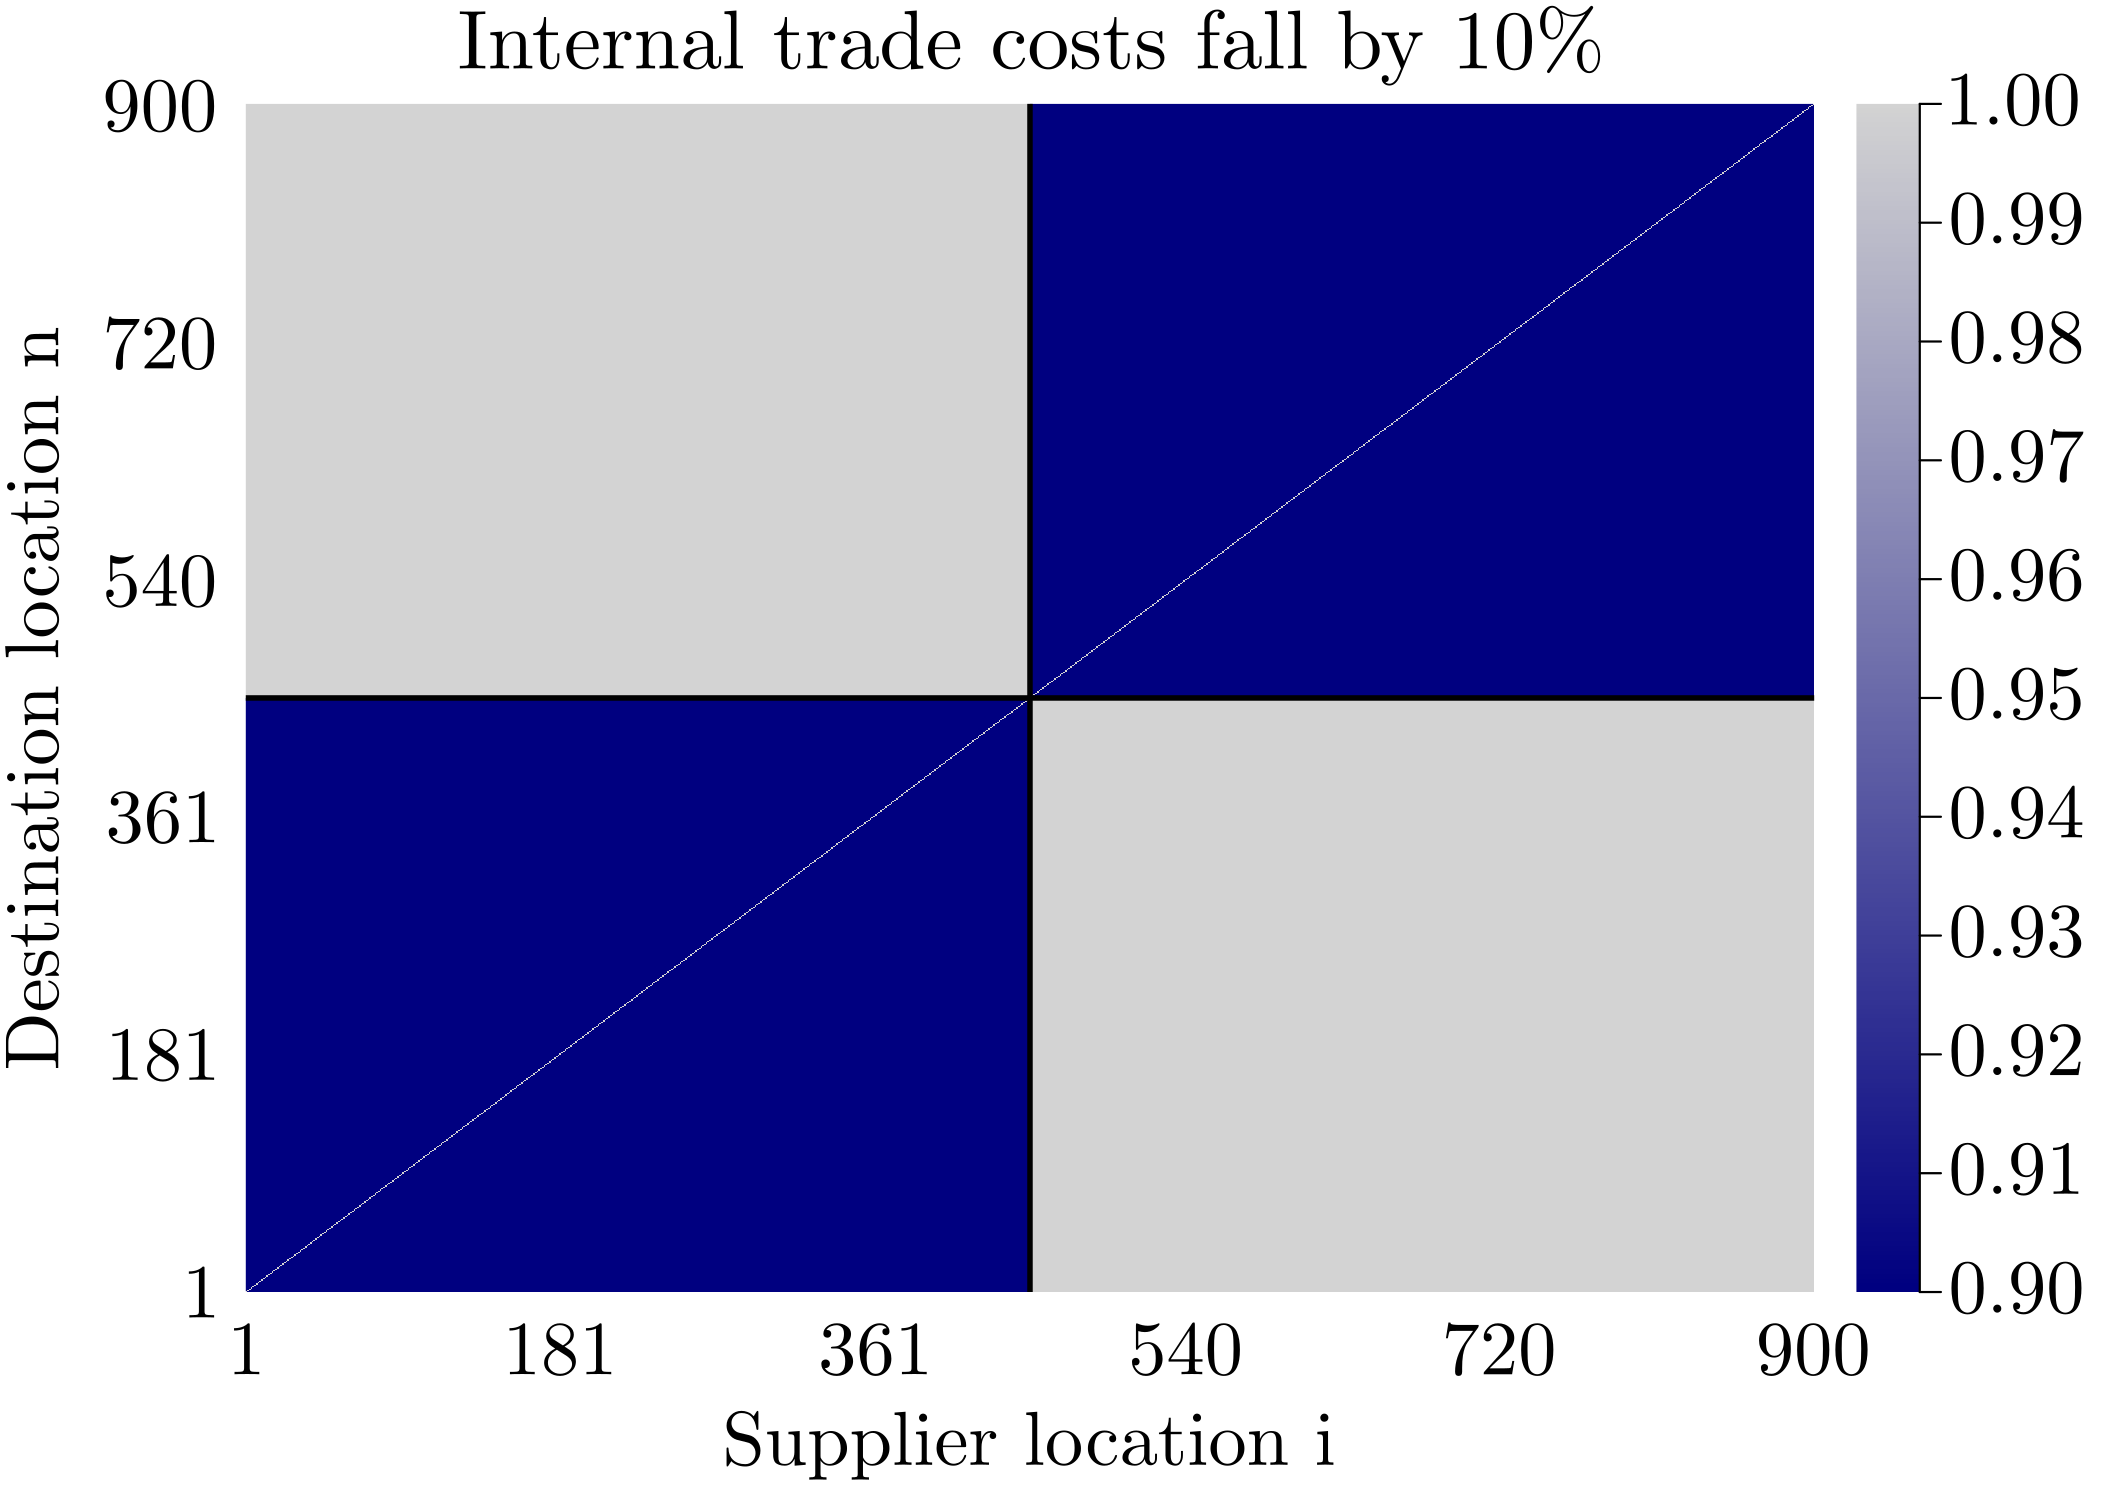
\includegraphics[height=0.60\textheight]
        {worked_example_shock_internal.png}
    \end{column}
  \end{columns}

  \vfill
\end{frame}

\begin{frame}[t]{Internal Trade: Results}
  \centering
  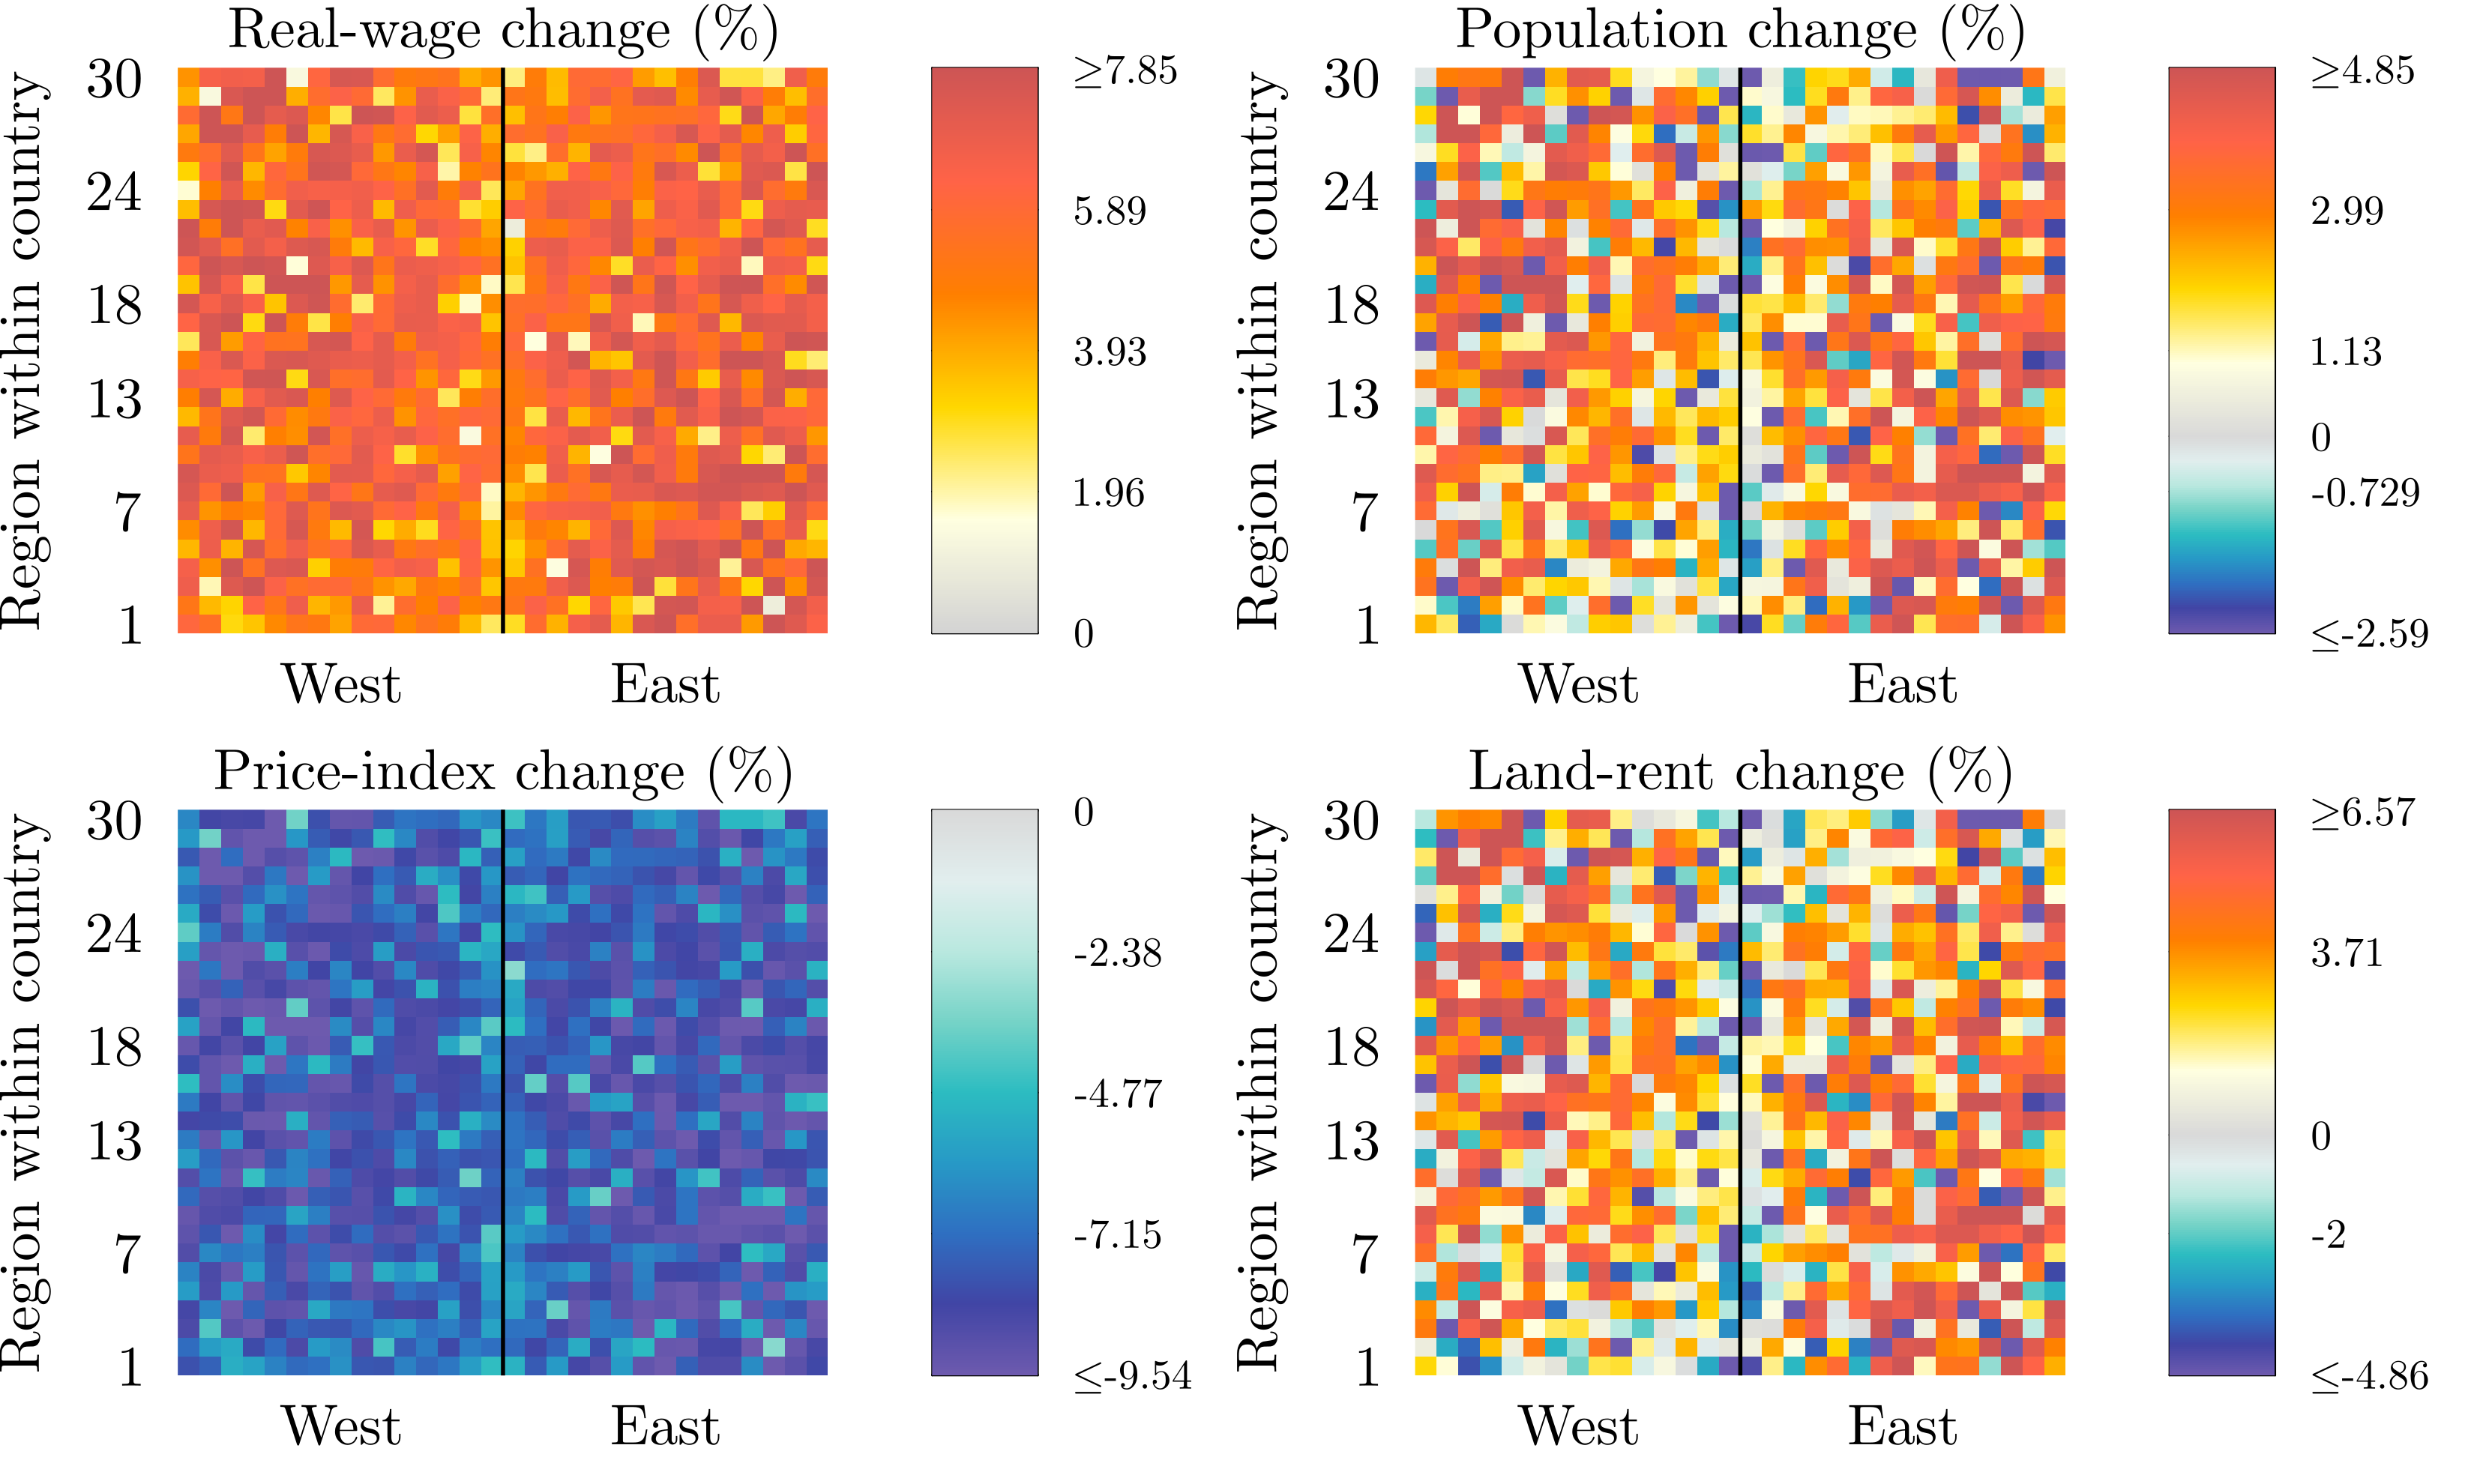
\includegraphics[height=0.62\textheight]
    {worked_example_results_internal.png}

  \footnotesize
  \B{Country inclusive-value welfare:}
  West \(+4.39\%\); East \(+4.41\%\).

  \scriptsize
  The baseline domestic interregional trade share is about \(30.8\%\).

\end{frame}

\begin{frame}[t]{Bilateral Border Liberalization: Shock}
  \small
  \begin{columns}[T,onlytextwidth]
    \begin{column}{0.45\textwidth}
      \B{Both countries reduce cross-border trade costs}
      \[
        \widehat d_{ni}
        =
        \begin{cases}
          0.9, & c(n)\neq c(i),\\
          1, & \text{otherwise}.
        \end{cases}
      \]
      \[
        \widehat{\mathbf A}
        =\widehat{\mathbf B}
        =\widehat{\mathbf H}
        =\mathbf1,
        \qquad
        \widehat F=\widehat{\bar{\mathbf L}}=1.
      \]
      Shipping costs fall by \(10\%\) in both directions across the national border.
      Domestic bilateral costs and all fundamentals remain fixed.
    \end{column}
    \begin{column}{0.51\textwidth}
      \centering
      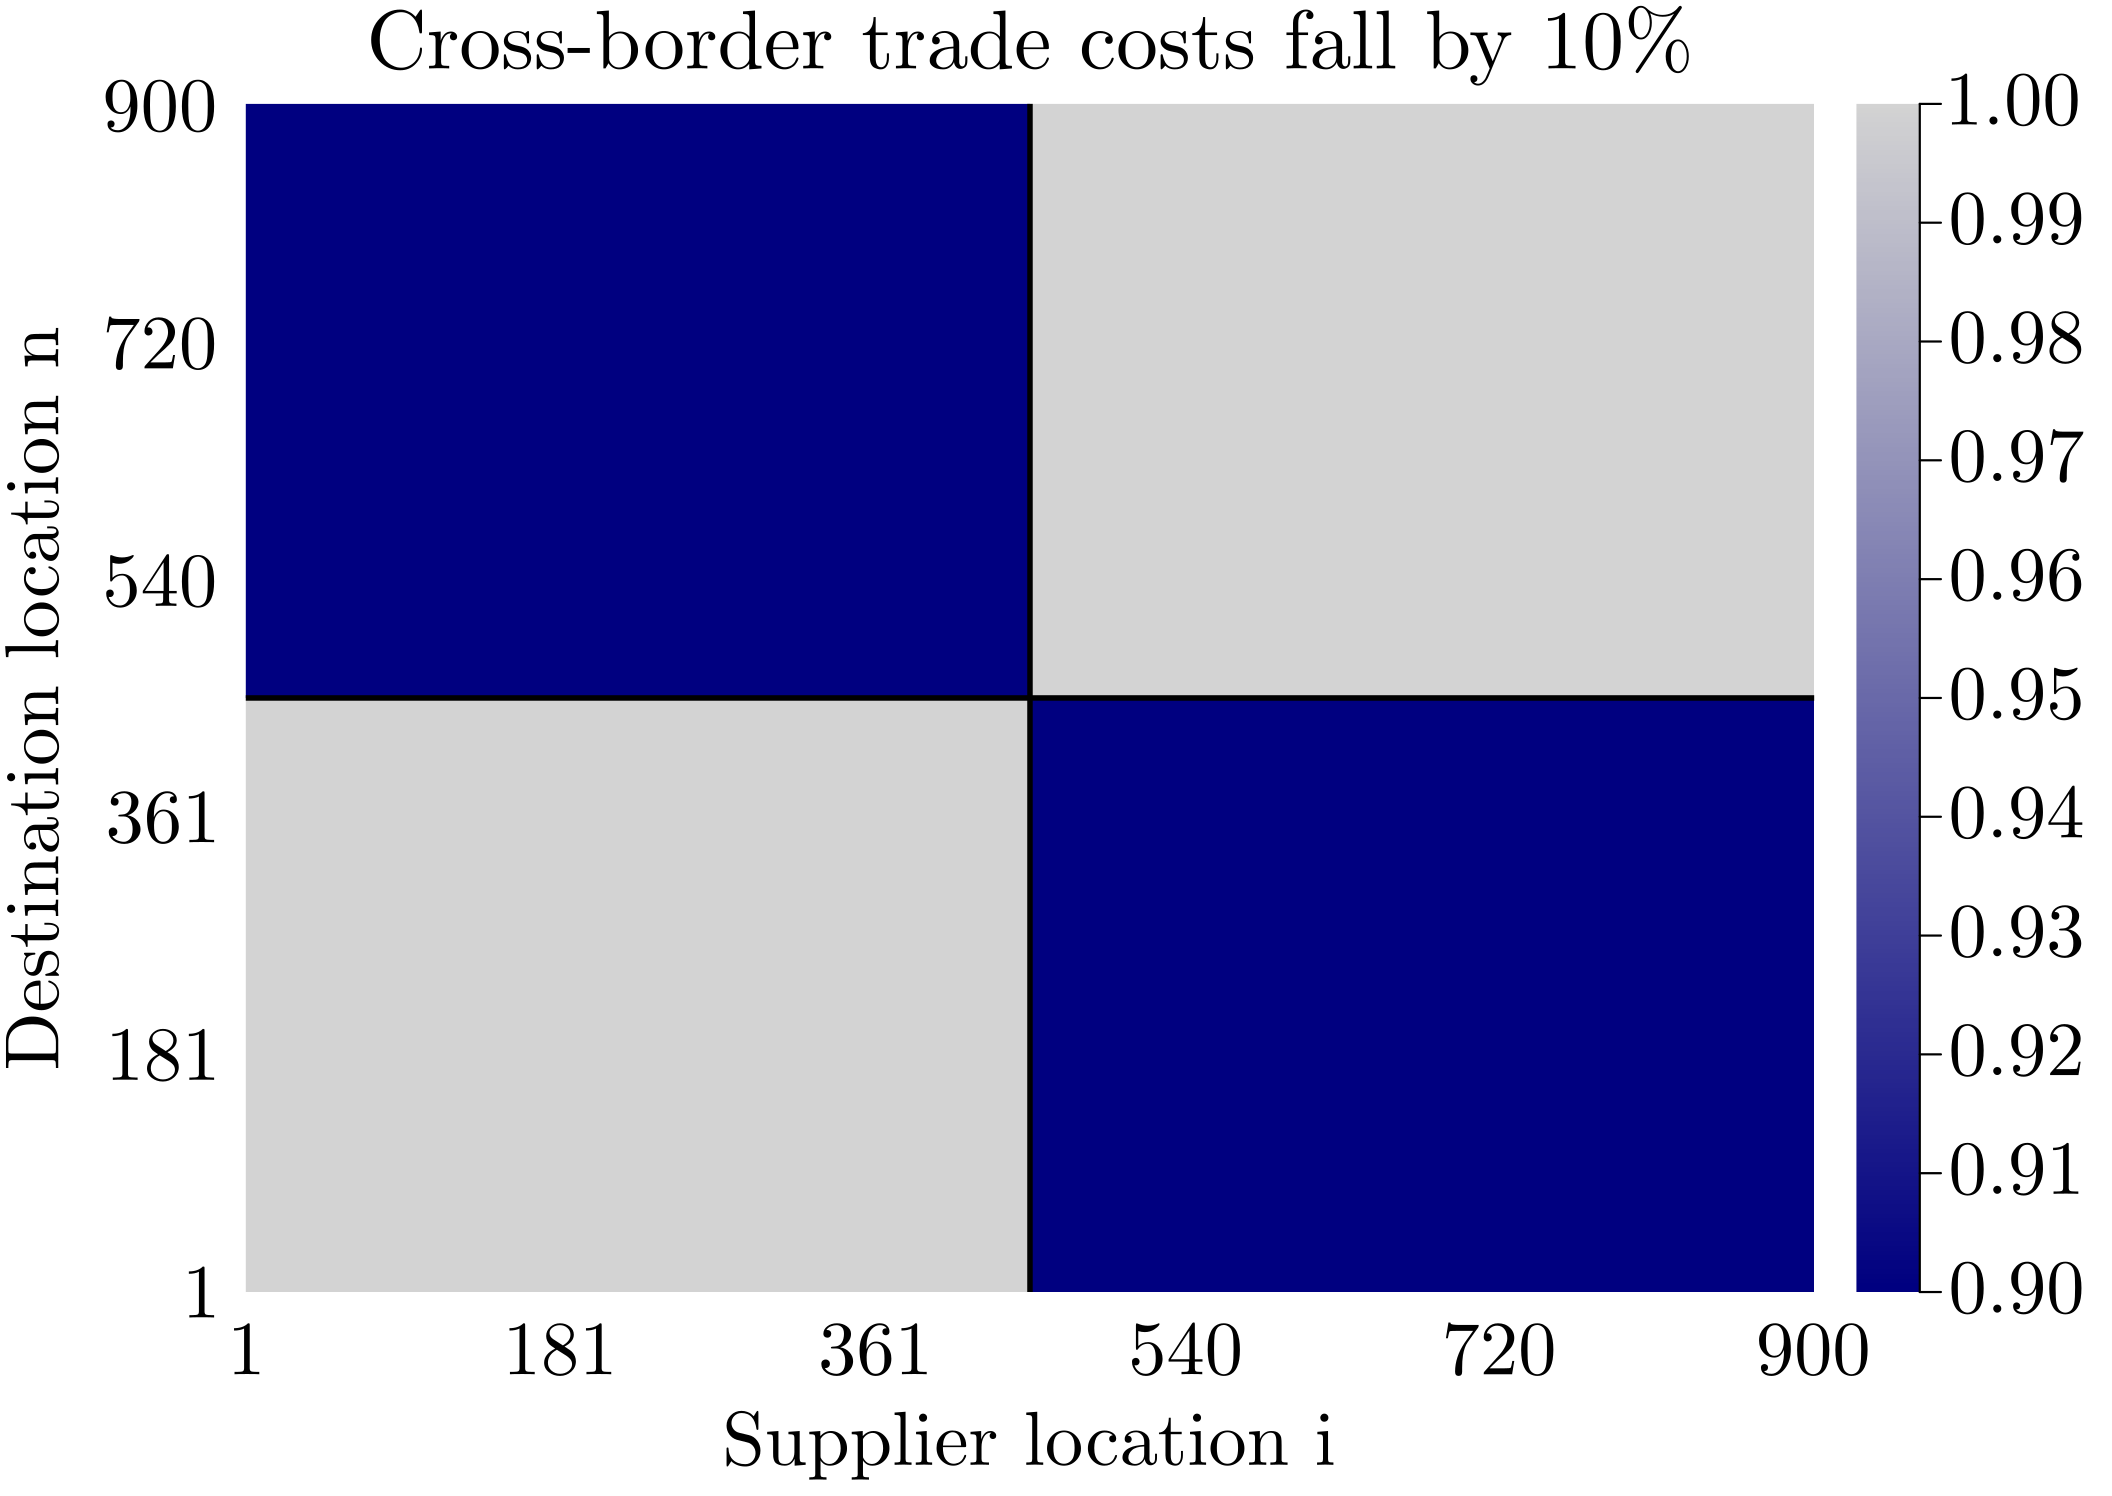
\includegraphics[height=0.60\textheight]
        {worked_example_shock_integration.png}
    \end{column}
  \end{columns}

  \vfill
\end{frame}

\begin{frame}[t]{External Trade: Results}
  \centering
  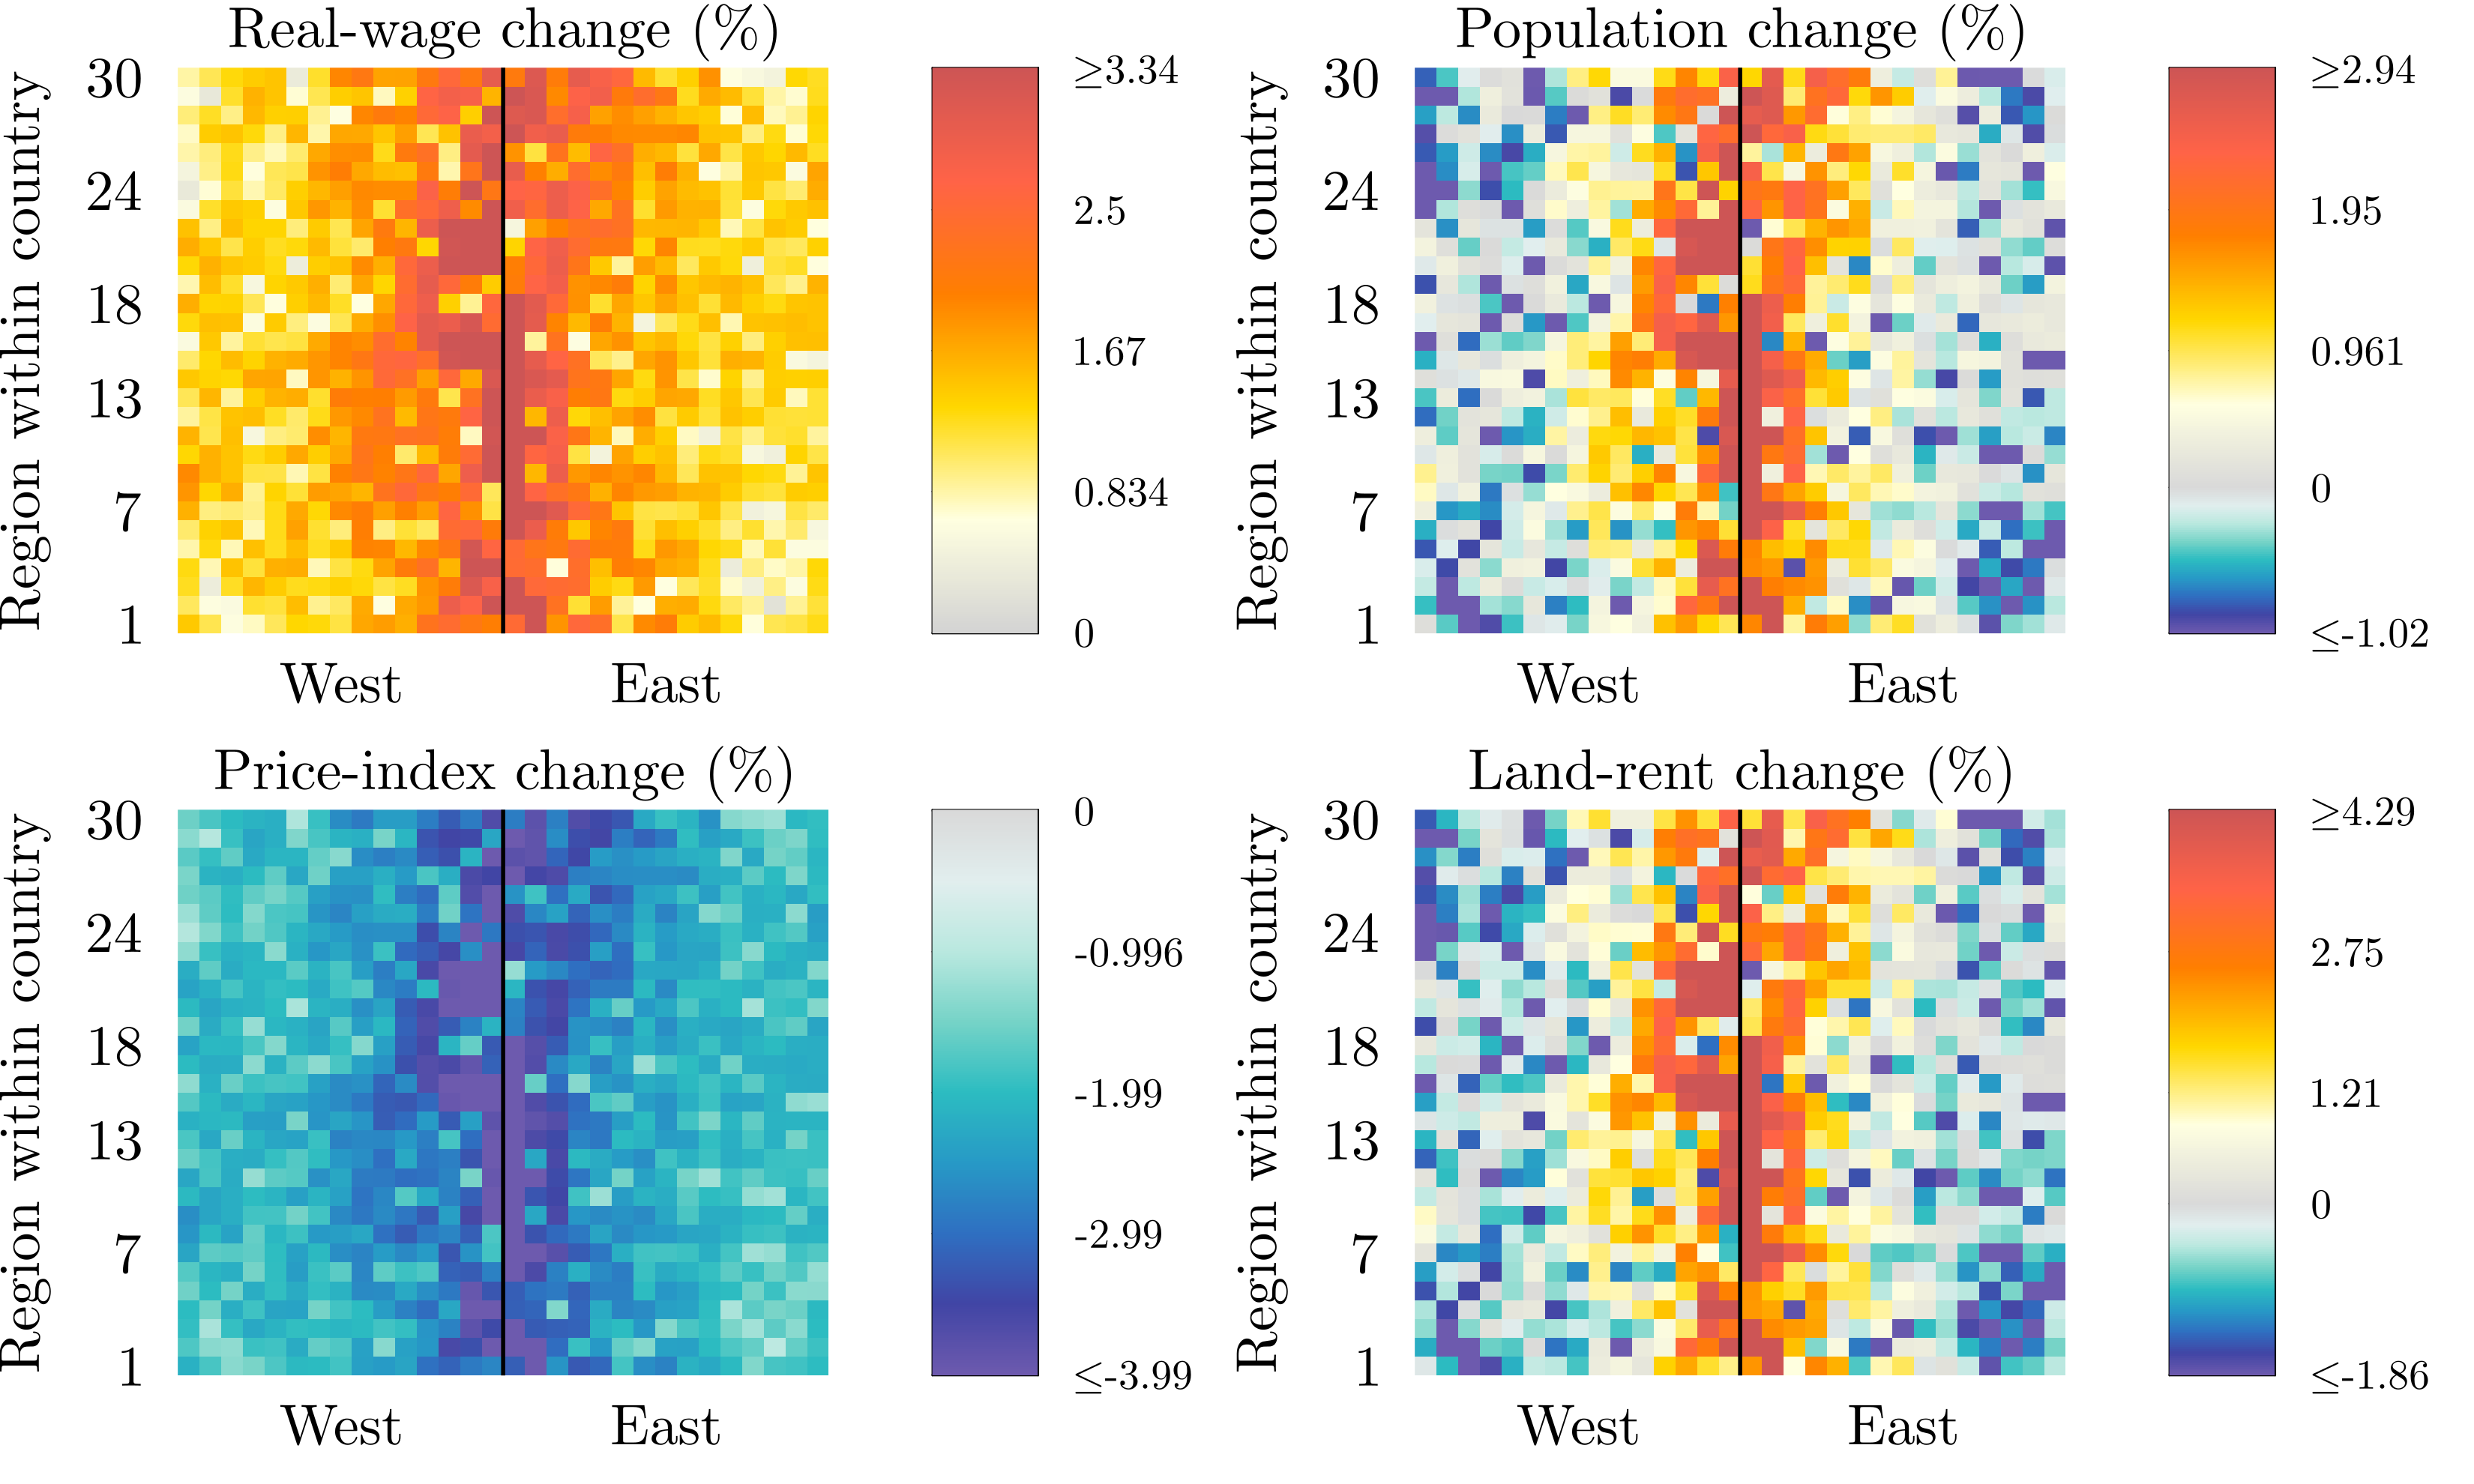
\includegraphics[height=0.62\textheight]
    {worked_example_results_integration.png}

  \footnotesize
  \B{Country inclusive-value welfare:}
  West \(+1.38\%\); East \(+1.33\%\).

  \scriptsize
  The baseline export share is about \(9.3\%\).

\end{frame}

\begin{frame}[t]{Road Construction: Shock}
  \footnotesize
  \setlength{\abovedisplayskip}{2pt}
  \setlength{\belowdisplayskip}{2pt}
  \begin{columns}[T,onlytextwidth]
    \begin{column}{0.45\textwidth}
      Let \(\delta_j\) be the unit traversal cost of grid cell \(j\):
      \[
        \widehat\delta_j
        =
        \begin{cases}
          0.50, & j\in\mathcal R,\\
          1, & \text{otherwise}.
        \end{cases}
      \]
      Recompute the lowest-cost route and effective distance for every
      origin--destination pair.
      The matrix \(\widehat{\mathbf d}\) is then constructed from the decline
      in effective distance:
      \begin{itemize}\setlength{\itemsep}{2pt}
        \item a larger distance reduction implies a lower trade-cost hat;
        \item unaffected OD pairs retain \(\widehat d_{ni}=1\).
      \end{itemize}
      \[
        \widehat{\mathbf A}
        =\widehat{\mathbf B}
        =\widehat{\mathbf H}
        =\mathbf1,
        \qquad
        \widehat F=\widehat{\bar{\mathbf L}}=1.
      \]
      The corridor can therefore improve market access beyond the locations
      lying directly on the road.
    \end{column}
    \begin{column}{0.51\textwidth}
      \centering
      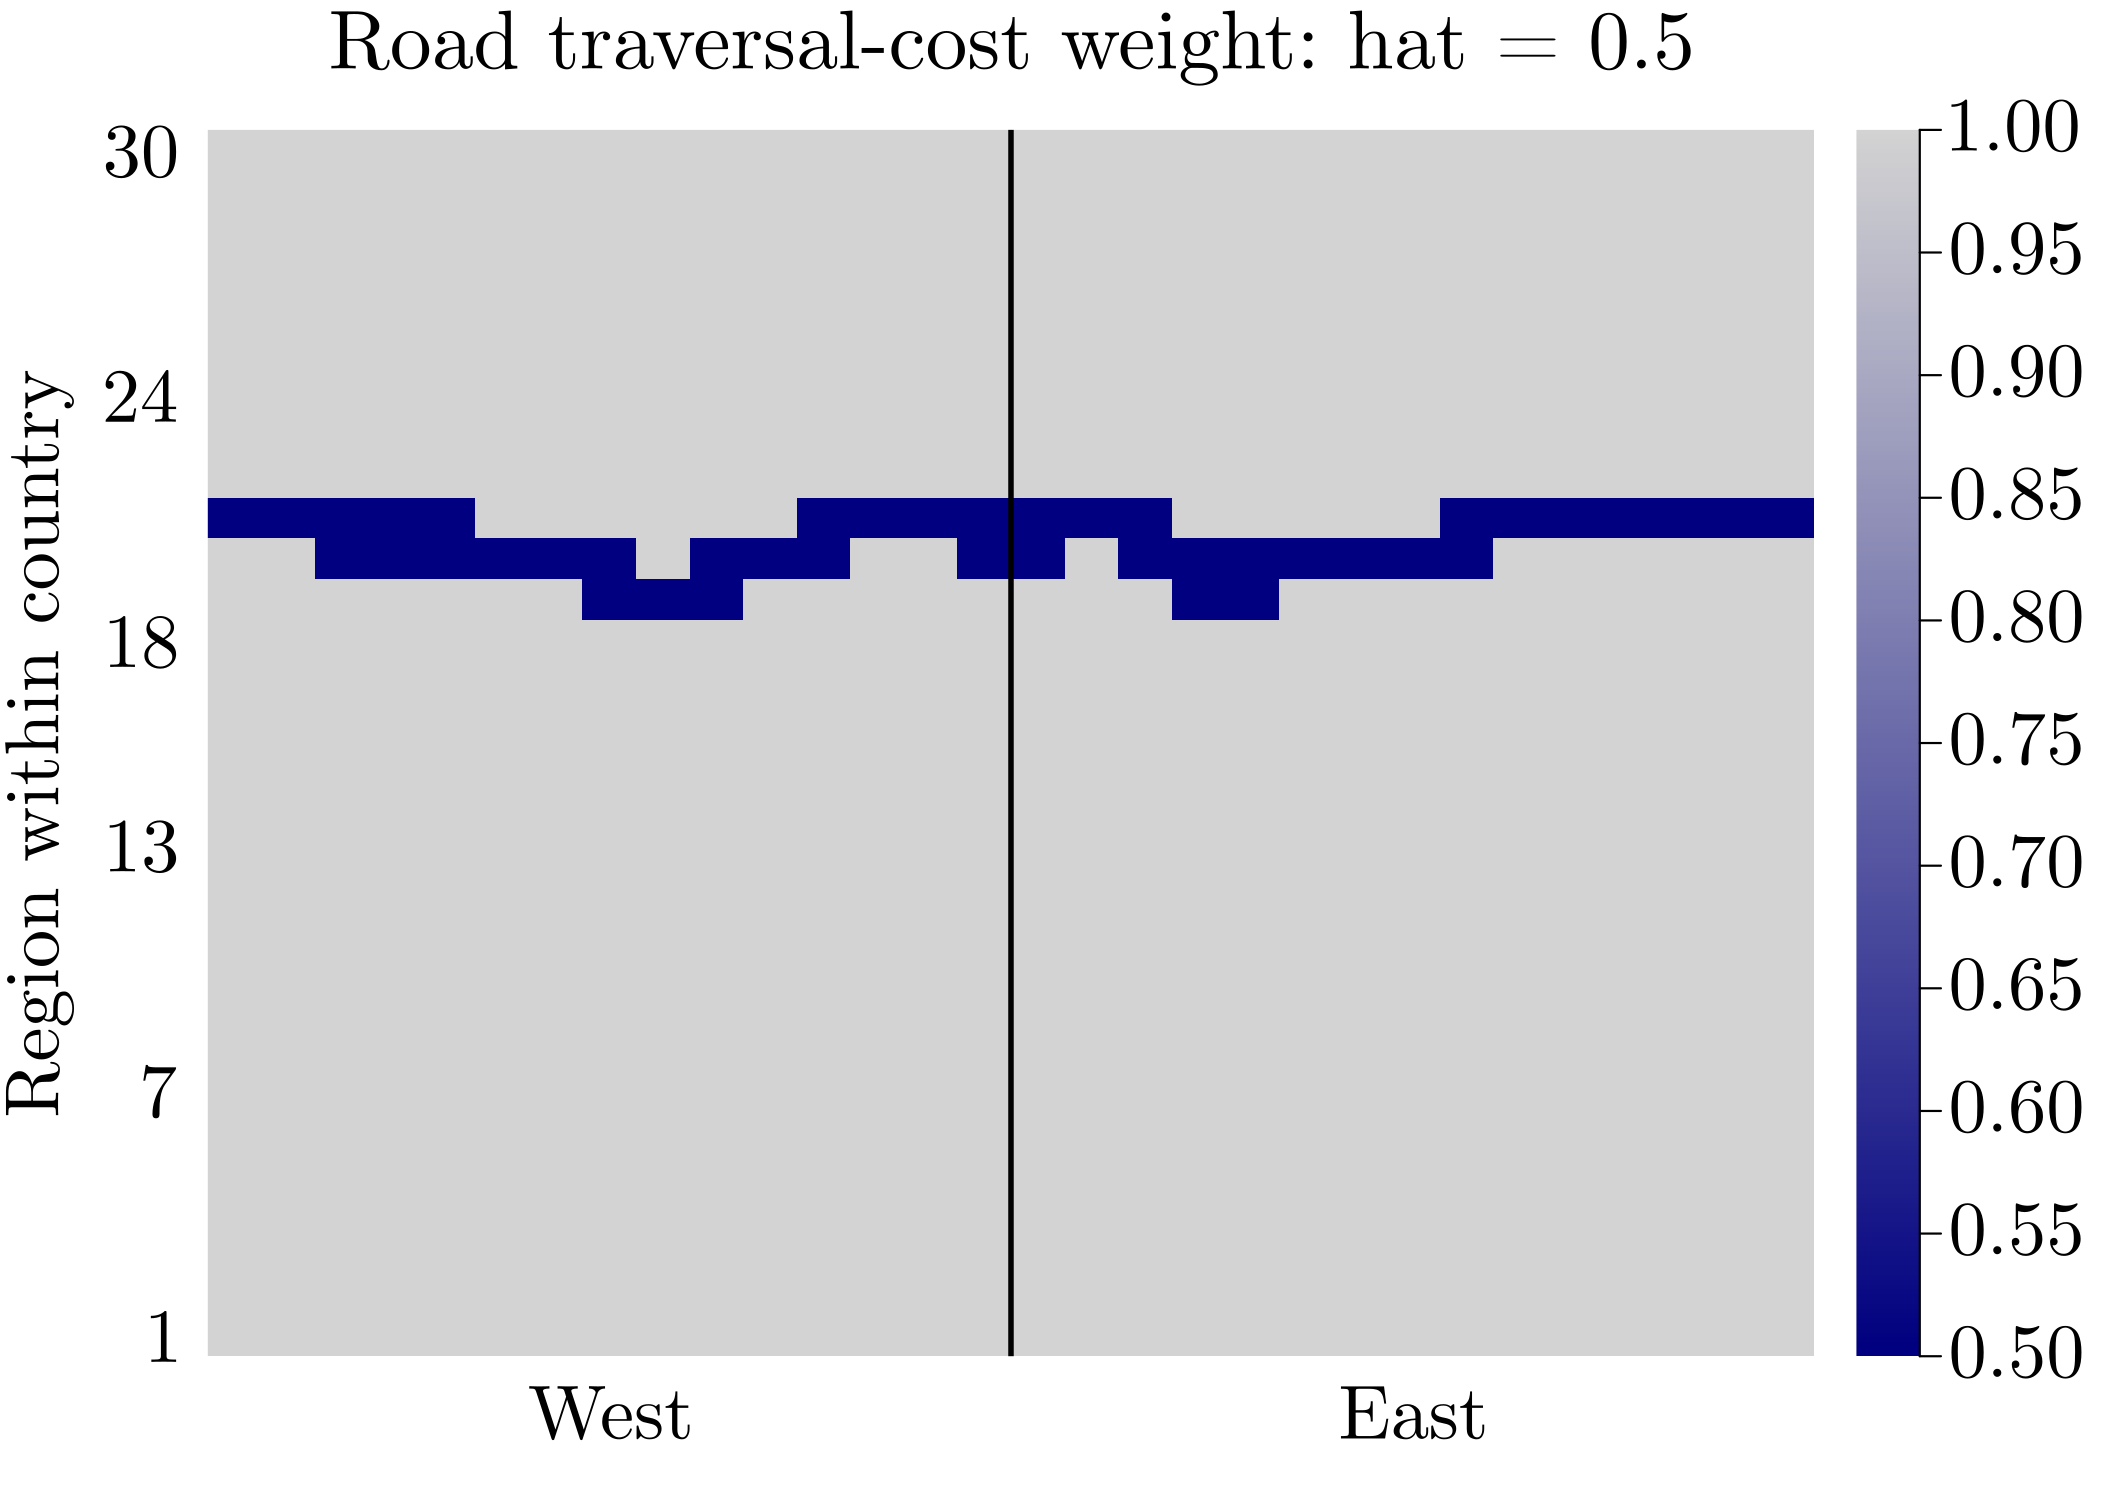
\includegraphics[height=0.55\textheight]
        {worked_example_shock_road.png}
    \end{column}
  \end{columns}

  \vfill
\end{frame}

\begin{frame}[t]{Road Construction: Results}
  \centering
  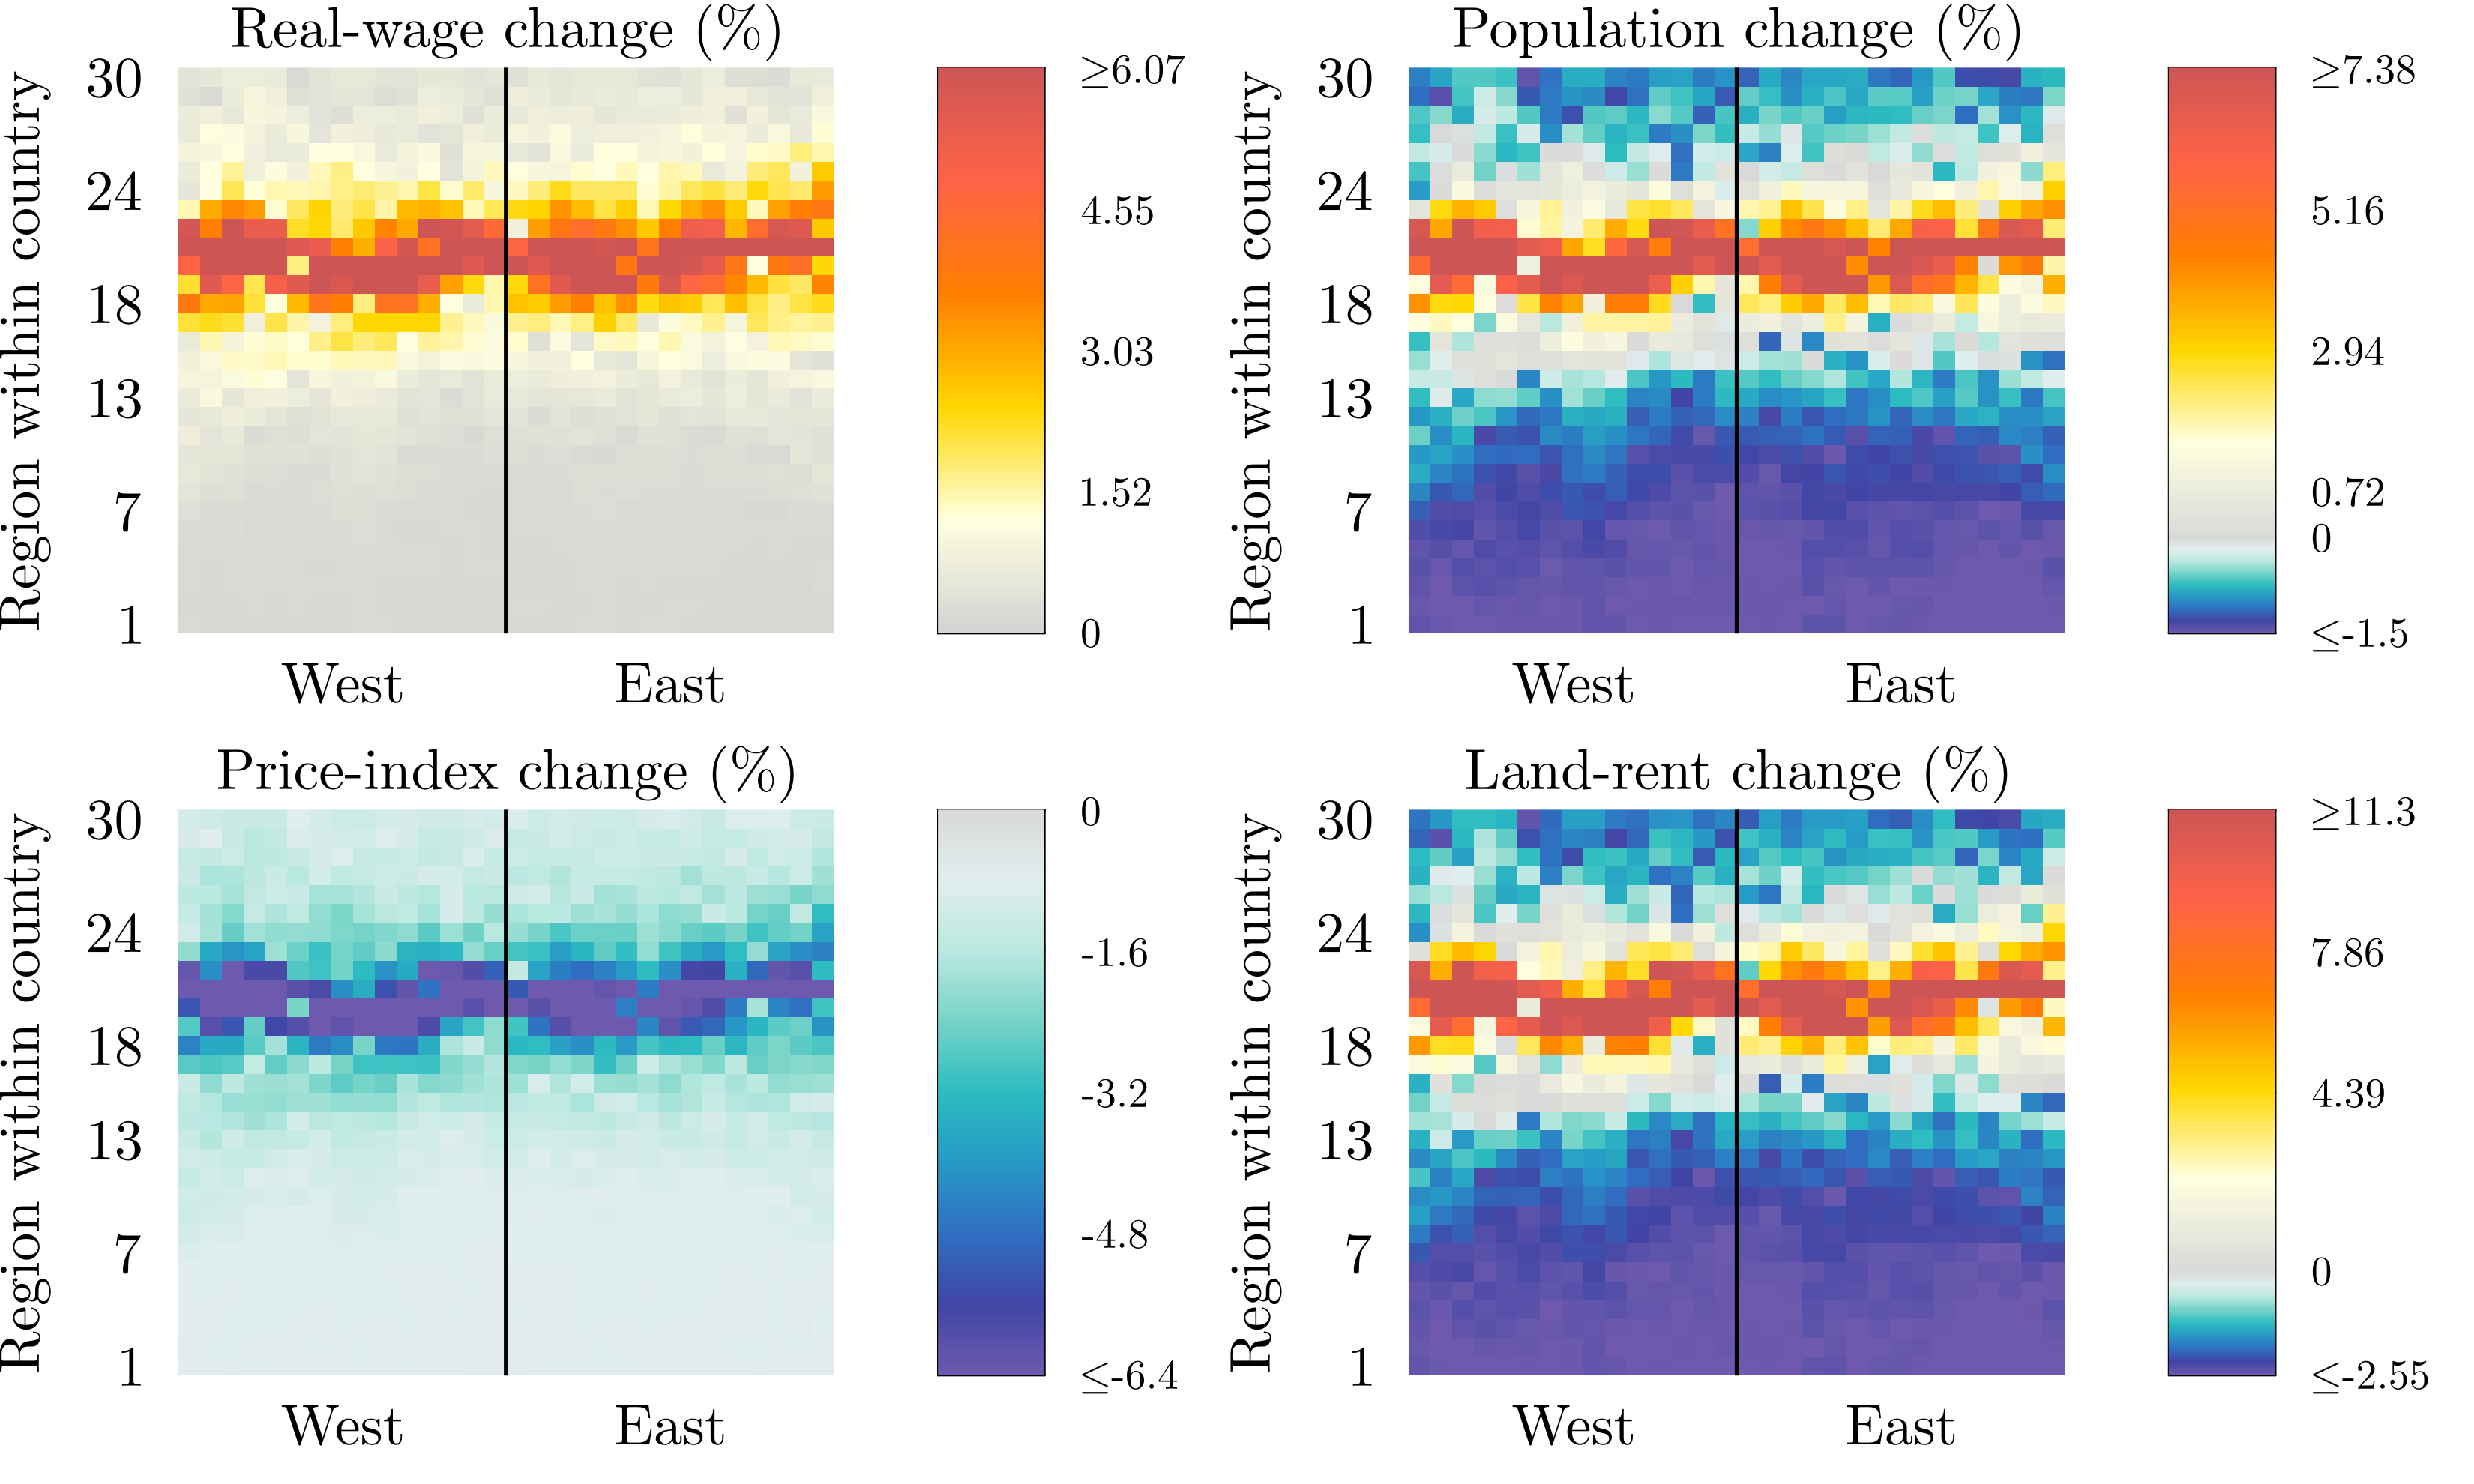
\includegraphics[height=0.60\textheight]
    {worked_example_results_road.png}

  \footnotesize
  \B{Country inclusive-value welfare:}
  West \(+1.14\%\); East \(+1.15\%\).

\end{frame}

\begin{frame}[t]{Development Zones: Shock}
  \small
  \begin{columns}[T,onlytextwidth]
    \begin{column}{0.45\textwidth}
      Let \(\mathcal Z=\mathcal Z_1\cup\mathcal Z_2\cup\mathcal Z_3\)
      denote three separated development zones inside West near the border.
      \[
        \widehat A_i
        =
        \begin{cases}
          1.20, & i\in\mathcal Z,\\
          1, & i\notin\mathcal Z.
        \end{cases}
      \]
      \[
        \widehat{\mathbf d}
        =\widehat{\mathbf B}
        =\widehat{\mathbf H}
        =\mathbf1,
        \qquad
        \widehat F=\widehat{\bar{\mathbf L}}=1.
      \]
      The three compact zones are generated with fixed seed
      \(20{,}260{,}725\). Productivity rises by \(20\%\) only inside them;
      no East location is directly treated.
    \end{column}
    \begin{column}{0.51\textwidth}
      \centering
      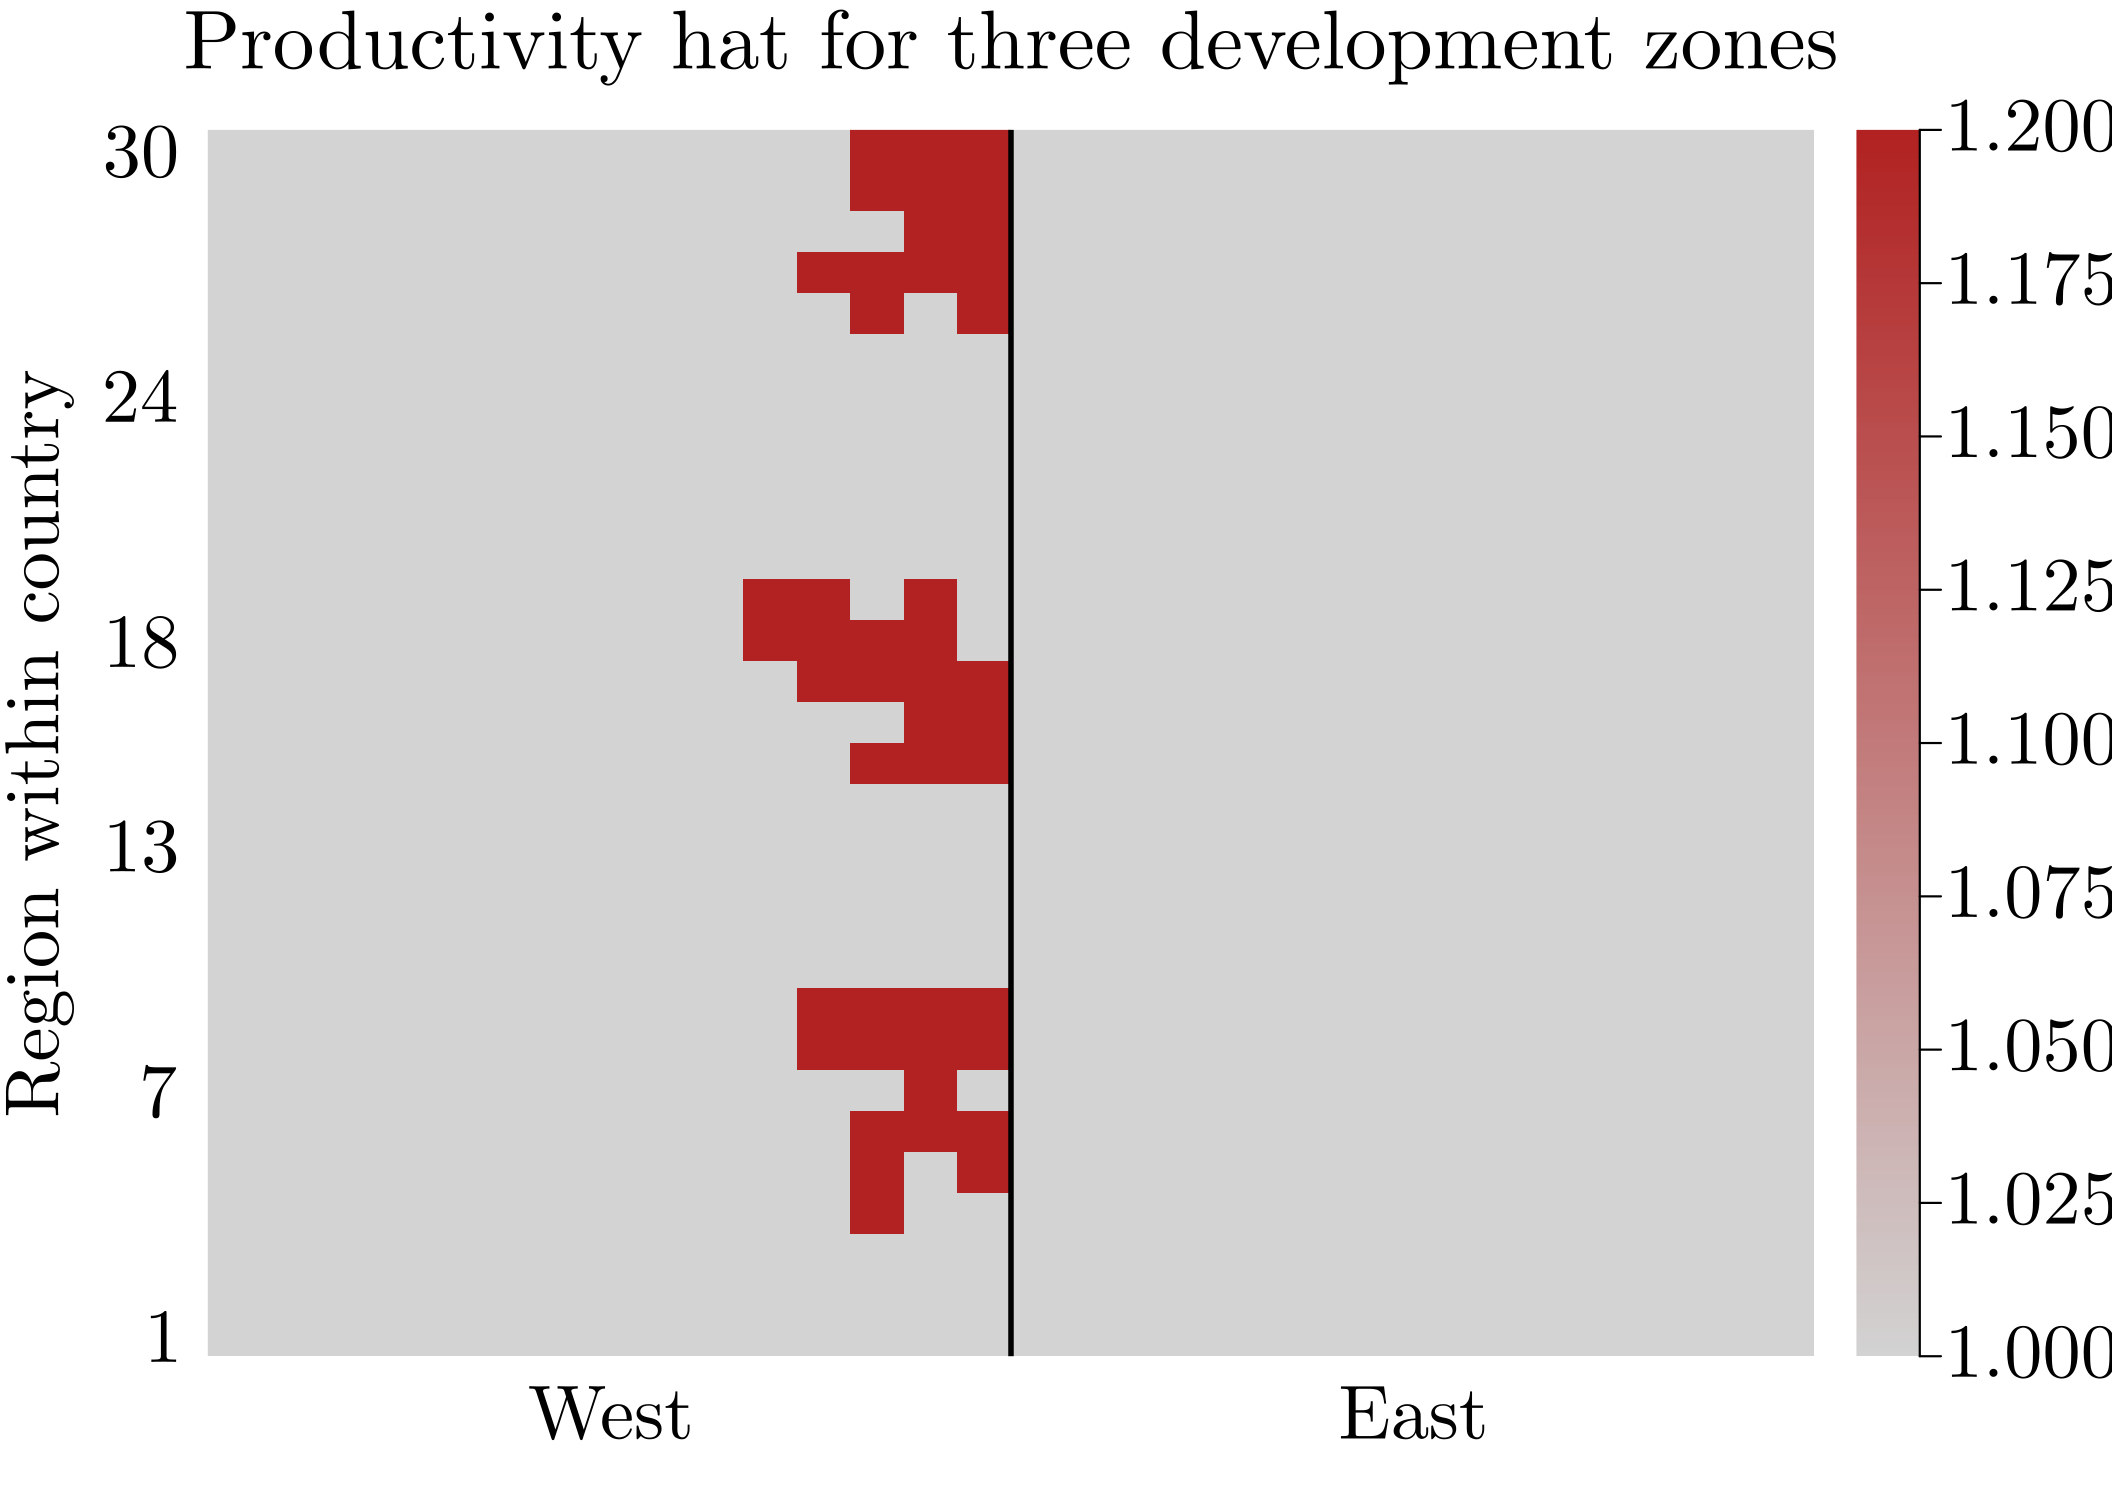
\includegraphics[height=0.60\textheight]
        {worked_example_shock_development.png}
    \end{column}
  \end{columns}

  \vfill
\end{frame}

\begin{frame}[t]{Development Zones: Results}
  \centering
  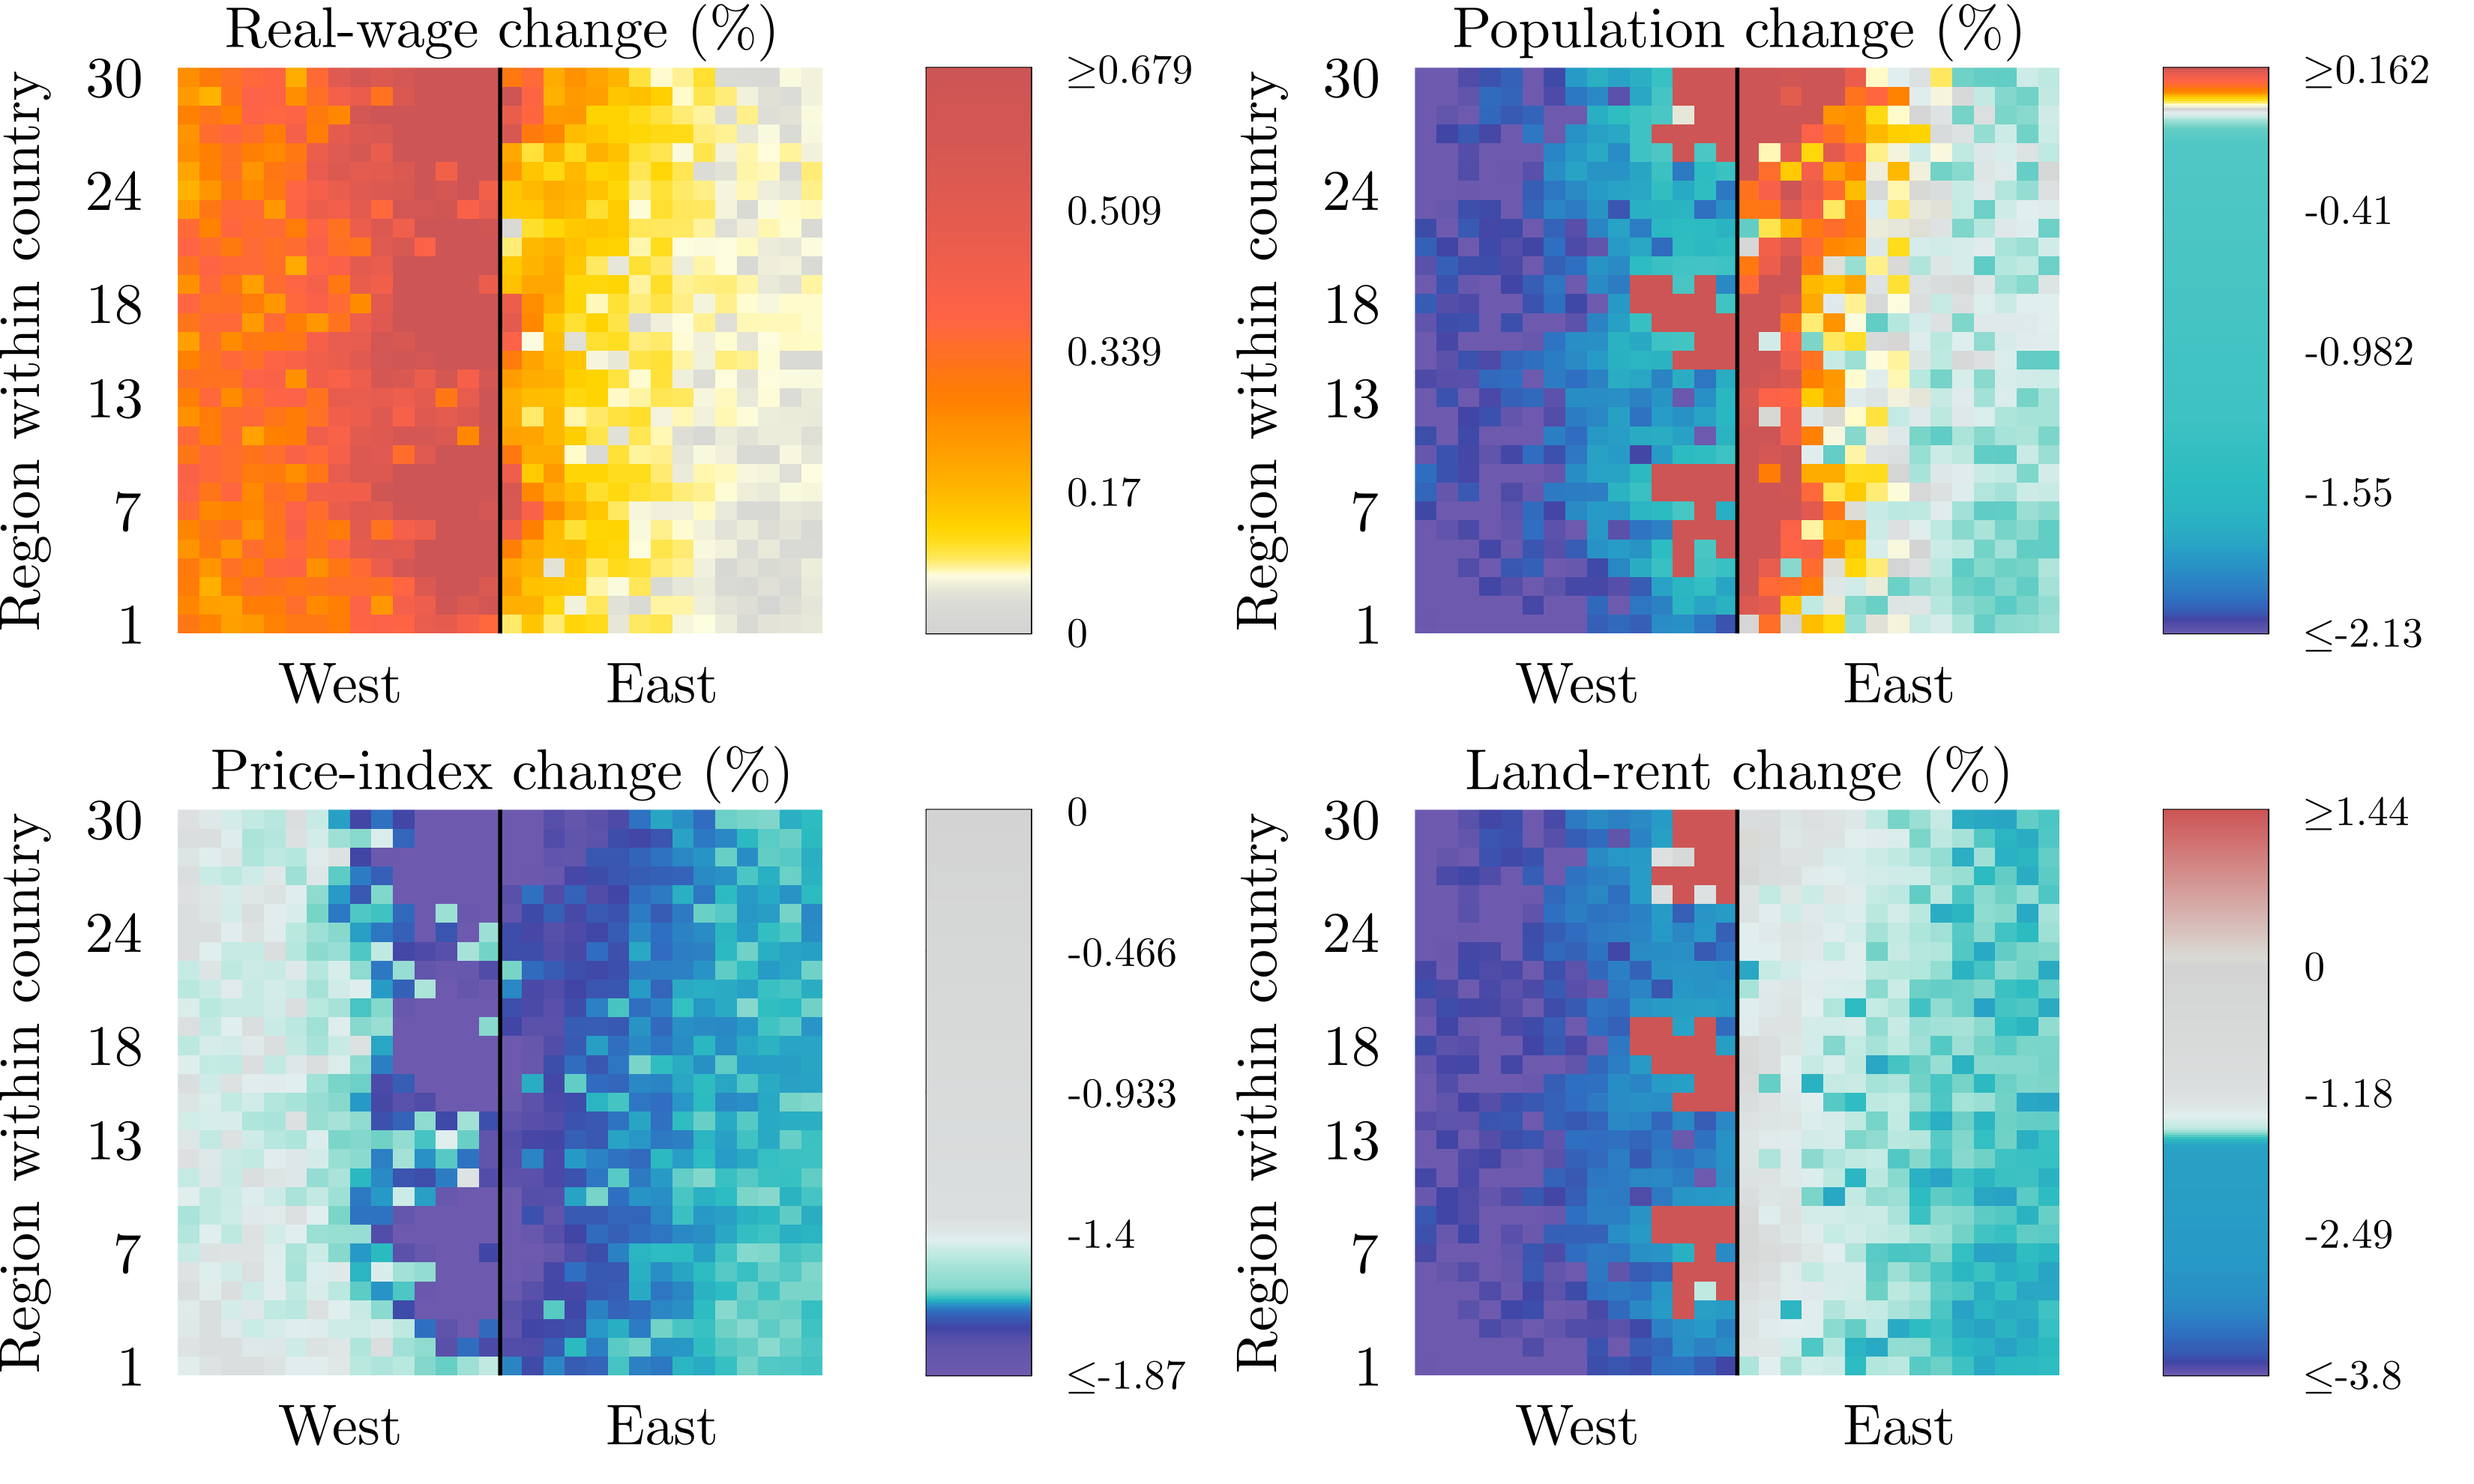
\includegraphics[height=0.62\textheight]
    {worked_example_results_development.png}

  \footnotesize
  \B{Country inclusive-value welfare:}
  West \(+1.74\%\); East \(+0.09\%\).

  \scriptsize
  East is untreated; its smaller, spatially varying responses arise through
  trade spillovers.

\end{frame}

\begin{frame}{Comparing the Four Policy Experiments}
  \scriptsize
  \renewcommand{\arraystretch}{1.12}
  \setlength{\tabcolsep}{3pt}
  \begin{center}
  \begin{tabular}{
    >{\raggedright\arraybackslash}p{0.27\textwidth}
    >{\centering\arraybackslash}p{0.13\textwidth}
    >{\centering\arraybackslash}p{0.13\textwidth}
    >{\centering\arraybackslash}p{0.15\textwidth}
    >{\centering\arraybackslash}p{0.15\textwidth}}
    \toprule
    Counterfactual and shock & West welfare & East welfare
      & \multicolumn{2}{c}{Mean absolute regional population change} \\
    \cmidrule(lr){4-5}
      & & & West & East \\
    \midrule
    \shortstack[l]{internal trade liberalization\\
      \(\widehat d^{\,\mathrm{dom}}=0.9\)}
      & \(+4.39\%\) & \(+4.41\%\) & \(2.15\%\) & \(2.36\%\) \\[1.5pt]
    \shortstack[l]{bilateral border liberalization\\
      \(\widehat d^{\,\mathrm{int}}=0.9\)}
      & \(+1.38\%\) & \(+1.33\%\) & \(0.84\%\) & \(0.89\%\) \\[1.5pt]
    \shortstack[l]{road construction\\
      \(\widehat\delta=0.5\) on the corridor}
      & \(+1.14\%\) & \(+1.15\%\) & \(1.61\%\) & \(1.70\%\) \\[1.5pt]
    \shortstack[l]{border development zones\\
      \(\widehat A=1.2\) inside the zones}
      & \(+1.74\%\) & \(+0.09\%\) & \(3.56\%\) & \(0.08\%\) \\
    \bottomrule
  \end{tabular}
  \end{center}

  \vspace{0.1em}
  \[
    \text{Mean absolute population change in }c
    =\sum_{n\in c}\lambda_n\,100\lvert\widehat L_n-1\rvert.
  \]

  \vspace{-0.4em}
  \B{Interpretation}
  \begin{itemize}\setlength{\itemsep}{2pt}
    \item Both trade experiments cut affected costs by \(10\%\). Internal
      liberalization applies to domestic nonlocal flows, a larger baseline
      expenditure share than cross-border trade.
    \item The corridor changes market access through the full lowest-cost-route network.
    \item West-side border zones directly raise local productivity and attract workers.
  \end{itemize}
\end{frame}

\section{Part V: Extensions}

\partdivider{V}{Extensions}

\setcounter{subsection}{0}

\subsection{Module 1: Preferences}

\begin{frame}{Extension Menu}
  \scriptsize
  \setlength{\tabcolsep}{3pt}
  \B{Baseline:} one-sector CES consumption, housing, exogenous amenities,
  and homogeneous households.

  \smallskip
  \renewcommand{\arraystretch}{1.15}
  \begin{center}
  \begin{tabular}{
    >{\raggedright\arraybackslash}p{0.20\textwidth}
    >{\centering\arraybackslash}p{0.34\textwidth}
    >{\raggedright\arraybackslash}p{0.37\textwidth}}
    \toprule
    Name & Representative formulation & Economic mechanism \\
    \midrule
    Multiple sectors
      & \(\displaystyle
          C_n=\prod_j\left(\frac{C_n^j}{\alpha_n^j}\right)^{\alpha_n^j}\)
      & Sectoral shocks, specialization, and structural transformation. \\
    \addlinespace[2pt]
    Nonhomothetic preferences
      & \(\displaystyle C_n=\prod_j(C_n^j-\bar c_j)^{\alpha_j}\)
      & Income-dependent expenditure shares and regional demand. \\
    \addlinespace[2pt]
    Endogenous amenities
      & \(\displaystyle B_n=\bar B_nL_n^{\eta_B}\)
      & City size, congestion, and place-based policies. \\
    \addlinespace[2pt]
    Quality choice
      & \(\displaystyle
          C_n=\left[\sum_i\int
          (q_{ni}(j)c_{ni}(j))^{\frac{\sigma-1}{\sigma}}dj
          \right]^{\frac{\sigma}{\sigma-1}}\)
      & Quality upgrading and income-dependent trade. \\
    \bottomrule
  \end{tabular}
  \end{center}
\end{frame}

\subsection{Module 2: Production Technology}

\begin{frame}{Extension Menu}
  \scriptsize
  \setlength{\tabcolsep}{3pt}
  \B{Baseline:} labor-only production with fixed costs, exogenous productivity,
  and no input--output linkages.

  \smallskip
  \renewcommand{\arraystretch}{1.08}
  \begin{center}
  \begin{tabular}{
    >{\raggedright\arraybackslash}p{0.19\textwidth}
    >{\centering\arraybackslash}p{0.35\textwidth}
    >{\raggedright\arraybackslash}p{0.37\textwidth}}
    \toprule
    Name & Representative formulation & Economic mechanism \\
    \midrule
    Constant versus increasing returns
      & \(\displaystyle
          x_i=A_i\ell_i
          \quad\text{vs.}\quad
          \ell_i=F+\frac{x_i}{A_i}\)
      & Firm scale, entry, and spatial concentration. \\
    \addlinespace[1pt]
    Input--output linkages
      & \(\displaystyle
          c_i^j=\frac{1}{A_i^j}w_i^{\beta_i^j}
          \prod_k(P_i^k)^{\gamma_i^{kj}}\)
      & Supply-chain propagation and local multipliers. \\
    \addlinespace[1pt]
    Multiple factors
      & \(\displaystyle
          c_i^j=\frac{1}{A_i^j}\prod_f(w_i^f)^{\beta_{jf}}\)
      & Factor intensity and distributional incidence. \\
    \addlinespace[1pt]
    Endogenous productivity
      & \(\displaystyle
          \begin{aligned}
            A_i&=\bar A_i\mathcal K_i^\eta,\\[-2pt]
            \mathcal K_i&=\sum_nK_{in}L_n
          \end{aligned}\)
      & Agglomeration and local-policy multipliers. \\
    \addlinespace[1pt]
    Firm heterogeneity
      & \(\displaystyle
          \varphi\sim G_i(\varphi),\qquad
          \Pi_{ni}(\varphi)\geq w_if_{ni}\)
      & Selection, export entry, and firm reallocation. \\
    \addlinespace[1pt]
    Fixed local production factors
      & \(\displaystyle Y_i=A_iL_i^\beta Q_i^{1-\beta}\)
      & Capacity constraints, rents, and specialization. \\
    \bottomrule
  \end{tabular}
  \end{center}
\end{frame}

\subsection{Module 3: Commodity Trade}

\begin{frame}{Extension Menu}
  \scriptsize
  \setlength{\tabcolsep}{3pt}
  \B{Baseline:} differentiated varieties, iceberg trade costs, one traded
  sector, anonymous market interaction, and no explicit transport network.

  \smallskip
  \renewcommand{\arraystretch}{1.06}
  \begin{center}
  \begin{tabular}{
    >{\raggedright\arraybackslash}p{0.19\textwidth}
    >{\centering\arraybackslash}p{0.35\textwidth}
    >{\raggedright\arraybackslash}p{0.37\textwidth}}
    \toprule
    Name & Representative formulation & Economic mechanism \\
    \midrule
    Eaton--Kortum sourcing
      & \(\displaystyle
          \pi_{ni}=
          \frac{A_i^{EK}(d_{ni}c_i)^{-\theta}}
          {\sum_kA_k^{EK}(d_{nk}c_k)^{-\theta}}\)
      & Ricardian comparative advantage and geography. \\
    \addlinespace[1pt]
    Fixed export costs
      & \(\displaystyle
          \begin{aligned}
            \pi_{ni}(\omega)
              &=\frac{r_{ni}(\omega)}{\sigma}-w_if_{ni},\\[-2pt]
            \text{export}
              &\iff \pi_{ni}(\omega)\geq0
          \end{aligned}\)
      & Export entry and the extensive trade margin. \\
    \addlinespace[1pt]
    Buyer--seller matching
      & \(\displaystyle
          \mathcal R_{ni}
          =\chi_{ni}\mathcal S_i^\eta
          \mathcal B_n^{1-\eta}\)
      & Search frictions, firm-to-firm links, and granular trade. \\
    \addlinespace[1pt]
    Transport networks
      & \(\displaystyle
          d_{ni}=\min_{\mathcal P_{ni}}
          \prod_{(r,s)\in\mathcal P_{ni}}\delta_{rs}\)
      & Roads, railways, ports, and rerouting. \\
    \addlinespace[1pt]
    Asymmetric trade costs
      & \(\displaystyle d_{ni}\neq d_{in}\)
      & Directional geography and asymmetric market access. \\
    \addlinespace[1pt]
    Nontraded goods
      & \(\displaystyle d_{ni}^{N}=\infty,\quad n\neq i\)
      & Local services and expenditure multipliers. \\
    \bottomrule
  \end{tabular}
  \end{center}
\end{frame}

\subsection{Module 4: Technology for Idea Flows}

\begin{frame}{Extension Menu}
  \scriptsize
  \setlength{\tabcolsep}{3pt}
  \B{Baseline:} no idea flows and exogenous local productivity.

  \smallskip
  \renewcommand{\arraystretch}{1.14}
  \begin{center}
  \begin{tabular}{
    >{\raggedright\arraybackslash}p{0.20\textwidth}
    >{\centering\arraybackslash}p{0.34\textwidth}
    >{\raggedright\arraybackslash}p{0.37\textwidth}}
    \toprule
    Name & Representative formulation & Economic mechanism \\
    \midrule
    Localized knowledge spillovers
      & \(\displaystyle
          A_i=\bar A_i\left(\sum_nK_{in}S_n\right)^\eta\)
      & Innovation clusters and agglomeration. \\
    \addlinespace[2pt]
    Exogenous technology diffusion
      & \(\displaystyle
          A_{i,t+1}=(1-\delta_A)A_{it}
          +\sum_n\omega_{ni}A_{nt}\)
      & Technology diffusion and regional convergence. \\
    \addlinespace[2pt]
    Endogenous innovation
      & \(\displaystyle
          A_{i,t+1}=(1-\delta_A)A_{it}+\chi R_{it}^{\nu}\)
      & Innovation policy and long-run growth. \\
    \addlinespace[2pt]
    Technology adoption
      & \(\displaystyle
          A_{i,t+1}=A_{it}+\rho_i(A_t^F-A_{it})\)
      & Catch-up and regional development. \\
    \addlinespace[2pt]
    Transferability of ideas
      & \(\displaystyle
          A_{ni}=\chi_{ni}A_i,\quad0<\chi_{ni}\leq1\)
      & Multinational production and technology transfer. \\
    \bottomrule
  \end{tabular}
  \end{center}
\end{frame}

\subsection{Module 5: Migration}

\begin{frame}{Extension Menu}
  \scriptsize
  \setlength{\tabcolsep}{3pt}
  \B{Baseline:} static destination choice, homogeneous workers, and residence
  equal to workplace.

  \smallskip
  \renewcommand{\arraystretch}{1.08}
  \begin{center}
  \begin{tabular}{
    >{\raggedright\arraybackslash}p{0.18\textwidth}
    >{\centering\arraybackslash}p{0.39\textwidth}
    >{\raggedright\arraybackslash}p{0.34\textwidth}}
    \toprule
    Name & Representative formulation & Economic mechanism \\
    \midrule
    Bilateral migration costs
      & \(\displaystyle
          m_{od}=
          \frac{(B_dV_d/\mu_{od})^\kappa}
          {\sum_k(B_kV_k/\mu_{ok})^\kappa}\)
      & Migration barriers and bilateral population flows. \\
    \addlinespace[1pt]
    Dynamic migration
      & \(\displaystyle
          \begin{aligned}
            V_{o,t}
              &=u_{o,t}+\beta E_t\max_d\{\\[-2pt]
              &\quad V_{d,t+1}-C_{od}+\epsilon_{od,t+1}\}
          \end{aligned}\)
      & Transition paths and adjustment speed. \\
    \addlinespace[1pt]
    Residence--workplace choice
      & \(\displaystyle
          \lambda_{rw}=
          \frac{V_{rw}^{\kappa}}{\sum_{s,k}V_{sk}^{\kappa}},
          \quad
          V_{rw}=\frac{B_rw_w}
          {P_r^\alpha r_r^{1-\alpha}d_{rw}}\)
      & Commuting and local labor-market spillovers. \\
    \addlinespace[1pt]
    Worker heterogeneity
      & \(\displaystyle
          m_{od}^g=
          \frac{(B_d^gV_d^g/\mu_{od}^g)^{\kappa_g}}
          {\sum_k(B_k^gV_k^g/\mu_{ok}^g)^{\kappa_g}}\)
      & Sorting and heterogeneous policy incidence. \\
    \addlinespace[1pt]
    Transportation congestion
      & \(\displaystyle
          d_{rw}=\bar d_{rw}
          \left[1+\gamma\left(\frac{Q_{rw}}{K_{rw}}\right)^\nu\right]\)
      & Congestion pricing and infrastructure capacity. \\
    \bottomrule
  \end{tabular}
  \end{center}
\end{frame}

\subsection{Module 6: Endowments}

\begin{frame}{Extension Menu}
  \scriptsize
  \setlength{\tabcolsep}{3pt}
  \B{Baseline:} homogeneous labor, fixed housing stocks, fixed total
  population, and no mobile capital.

  \smallskip
  \renewcommand{\arraystretch}{1.08}
  \begin{center}
  \begin{tabular}{
    >{\raggedright\arraybackslash}p{0.20\textwidth}
    >{\centering\arraybackslash}p{0.34\textwidth}
    >{\raggedright\arraybackslash}p{0.37\textwidth}}
    \toprule
    Name & Representative formulation & Economic mechanism \\
    \midrule
    Multiple skill endowments
      & \(\displaystyle \sum_iL_i^g=\bar L^g,\quad g=1,\ldots,G\)
      & Skill abundance, sorting, and inequality. \\
    \addlinespace[1pt]
    Elastic housing supply
      & \(\displaystyle H_i=\bar H_i r_i^{\eta_i}\)
      & Zoning, city growth, and rent capitalization. \\
    \addlinespace[1pt]
    Mobile capital
      & \(\displaystyle R_i^K=R^K,\qquad\sum_iK_i=\bar K\)
      & Investment responses and regional convergence. \\
    \addlinespace[1pt]
    Capital accumulation
      & \(\displaystyle \Delta K_{it}=I_{it}-\delta K_{it}\)
      & Short-run versus long-run spatial effects. \\
    \addlinespace[1pt]
    Infrastructure endowments
      & \(\displaystyle
          d_{ni}=d_{ni}(K_e),\qquad
          \frac{\partial d_{ni}}{\partial K_e}<0\)
      & Infrastructure placement and network investment. \\
    \bottomrule
  \end{tabular}
  \end{center}
\end{frame}

\subsection{Module 7: Equilibrium}

\begin{frame}{Alternative Equilibrium Closures}
  \scriptsize
  \setlength{\tabcolsep}{3pt}
  \B{Baseline:} monopolistic competition with free entry, full general
  equilibrium, local rent rebates, and balanced trade.

  \smallskip
  \renewcommand{\arraystretch}{1.16}
  \begin{center}
  \begin{tabular}{
    >{\raggedright\arraybackslash}p{0.20\textwidth}
    >{\centering\arraybackslash}p{0.38\textwidth}
    >{\raggedright\arraybackslash}p{0.33\textwidth}}
    \toprule
    Name & Representative formulation & Economic mechanism \\
    \midrule
    Market structure
      & \(\displaystyle
          p_i=mc_i
          \quad\text{vs.}\quad
          p_i=\mu mc_i,\ \Pi_i=0\)
      & Markups, entry, variety, and returns to scale. \\
    \addlinespace[3pt]
    Equilibrium scope
      & \(\displaystyle
          \mathcal F(\mathbf z^{in};
          \bar{\mathbf z}^{out},\phi)=0
          \quad\text{vs.}\quad
          \mathcal F(\mathbf z;\phi)=0\)
      & Endogenous versus externally fixed prices, expenditures, and utility. \\
    \addlinespace[3pt]
    Land ownership and rent distribution
      & \(\displaystyle
          \begin{aligned}
            t_nL_n&=\sum_i s_{ni}r_iH_i,\\[-2pt]
            s_{ni}&:\ \text{fixed or endogenous}
          \end{aligned}\)
      & Rent ownership, capitalization, and welfare incidence. \\
    \addlinespace[3pt]
    Trade-balance closure
      & \(\displaystyle
          \begin{aligned}
            E_{it}&=w_{it}L_{it}+D_{it},\\[-2pt]
            D_{it}&=\bar D_{it}
            \quad\text{or}\quad
            (1+R_t)a_{it}-a_{i,t+1}
          \end{aligned}\)
      & External imbalances, saving, and borrowing. \\
    \bottomrule
  \end{tabular}
  \end{center}
\end{frame}

\subsection{Choosing an Extension}

\begin{frame}{A Practical Checklist}
  \small
  \setlength{\tabcolsep}{5pt}
  \renewcommand{\arraystretch}{1.22}
  \begin{center}
  \begin{tabular}{
    >{\raggedright\arraybackslash}p{0.42\textwidth}
    >{\raggedright\arraybackslash}p{0.50\textwidth}}
    \toprule
    Question & Modeling implication \\
    \midrule
    Which adjustment margin is missing?
      & Select the corresponding module extension. \\
    \addlinespace[3pt]
    Which new endogenous objects appear?
      & Add the relevant equilibrium equations. \\
    \addlinespace[3pt]
    Which new parameters are required?
      & Estimate or calibrate the associated elasticities. \\
    \addlinespace[3pt]
    Which additional data are needed?
      & Match new flows, prices, stocks, or group-level outcomes. \\
    \addlinespace[3pt]
    Does the extension change the counterfactual result?
      & Retain only quantitatively important mechanisms. \\
    \bottomrule
  \end{tabular}
  \end{center}
\end{frame}

\subsection{References}

\begin{frame}[t]{Core Literature and Online Resources}
  \fontsize{7.4}{8.7}\selectfont
  \begin{columns}[T,onlytextwidth]
    \begin{column}{0.64\textwidth}
      {\color{deepred}\bfseries Core references}

      \vspace{2pt}
      Redding, S. J., and E. Rossi-Hansberg. 2017.
      ``Quantitative Spatial Economics.''
      \emph{Annual Review of Economics}, 9: 21--58.

      \vspace{3pt}
      Allen, T., and C. Arkolakis. 2014.
      ``Trade and the Topography of the Spatial Economy.''
      \emph{Quarterly Journal of Economics}, 129(3): 1085--1140.

      \vspace{3pt}
      Dekle, R., J. Eaton, and S. Kortum. 2008.
      ``Global Rebalancing with Gravity.''
      \emph{IMF Staff Papers}, 55(3): 511--540.

      \vspace{3pt}
      Caliendo, L., and F. Parro. 2015.
      ``Estimates of the Trade and Welfare Effects of NAFTA.''
      \emph{Review of Economic Studies}, 82(1): 1--44.

      \vspace{3pt}
      Monte, F., S. J. Redding, and E. Rossi-Hansberg. 2018.
      ``Commuting, Migration, and Local Employment Elasticities.''
      \emph{American Economic Review}, 108(12): 3855--3890.

      \vspace{3pt}
      Caliendo, L., M. Dvorkin, and F. Parro. 2019.
      ``Trade and Labor Market Dynamics.''
      \emph{Econometrica}, 87(3): 741--835.

      \vspace{8pt}
      {\color{deepred}\bfseries Lecture repository}

      \vspace{2pt}
      Slides and replication code:\\[-1pt]
      \nolinkurl{https://github.com/ALLBLUEUK/}\\[-1pt]
      \nolinkurl{structural-modeling-for-economists/tree/main/}\\[-1pt]
      \nolinkurl{examples/quantitative-spatial-models-lecture}
    \end{column}

    \begin{column}{0.32\textwidth}
      {\color{deepred}\bfseries Online resources}

      \vspace{4pt}
      \textbf{Zi Wang}\\
      Structural Models and Numerical Methods in Economics\\[-1pt]
      \nolinkurl{https://github.com/WangZi-HKBU/econ7115}

      \vspace{6pt}
      \textbf{Treb Allen}\\
      Graduate Trade and Modern Spatial Economics\\[-1pt]
      \nolinkurl{https://sites.google.com/site/treballen/graduate-trade}

      \vspace{6pt}
      \textbf{Gabriel Ahlfeldt}\\
      Lectures in Quantitative Spatial Economics\\[-1pt]
      \nolinkurl{https://github.com/Ahlfeldt/}\\[-1pt]
      \nolinkurl{Lectures-Quantitative}\\[-1pt]
      \nolinkurl{SpatialEconomics}

      \vspace{6pt}
      \textbf{Quantitative Urban Models}\\
      Lectures and toolkits\\[-1pt]
      \nolinkurl{https://www.quantitativeurbanmodels.com/}
    \end{column}
  \end{columns}
\end{frame}

\appendix
\section{Appendix}

\begin{frame}[plain]
  \vfill
  \begin{center}
    {\color{oxfordblue}\LARGE\bfseries APPENDIX\par}
  \end{center}
  \vfill
\end{frame}

\subsection{Application Inputs}

\begin{frame}[label=baselineConstruction]{Baseline Settings for the Synthetic Data}
  \scriptsize
  \setlength{\tabcolsep}{5pt}
  \renewcommand{\arraystretch}{1.14}
  \begin{center}
  \begin{tabular}{
    >{\raggedright\arraybackslash}p{0.25\textwidth}
    >{\raggedright\arraybackslash}p{0.64\textwidth}}
    \toprule
    Model object & Setting used in the level simulation \\
    \midrule
    Geography and labor
      & \(30\times30=900\) regions; two countries;
        \(\bar L_c=50{,}000\) workers in each country \\
    Parameters
      & \(\alpha=0.75,\ \sigma=5,\ \kappa=1.5,\ F=1\) \\
    Productivity
      & \(\operatorname{sd}(\log A_i)=1.00\), normalized within country \\
    Amenities
      & \(B_i=1\) \\
    Housing
      & fixed local stock \(H_i=100\) \\
    Iceberg trade costs
      & distance elasticity \(0.35\); nonlocal factor \(2\);
        international-border factor \(2\); cross-country effective-distance
        normalization \(6.303\) \\
    Equilibrium closure
      & fixed country populations, balanced trade, and mobility within country \\
    \bottomrule
  \end{tabular}
  \end{center}

  \smallskip
  \[
    \{\mathbf A,\mathbf B,\mathbf H,\mathbf d,
      F,\bar{\mathbf L};\alpha,\sigma,\kappa\}
    \quad\longrightarrow\quad
    \{\mathbf w,\mathbf L,\mathbf P,
      \boldsymbol\pi,\boldsymbol\lambda\}.
  \]

  \centering\scriptsize
  The balanced-trade simulation approximately targets own-location,
  domestic-nonlocal, and foreign expenditure shares of
  \(60\%\), \(30\%\), and \(10\%\)
  (Li et al., 2025).

  \vfill
  \visualbutton{visFundamentals}{View fundamental maps}
  \hfill
  \hfill\backlink{appInputs}{Back to Inputs}
\end{frame}

\begin{frame}[label=visFundamentals]{Baseline Regional Fundamentals}
  \centering
  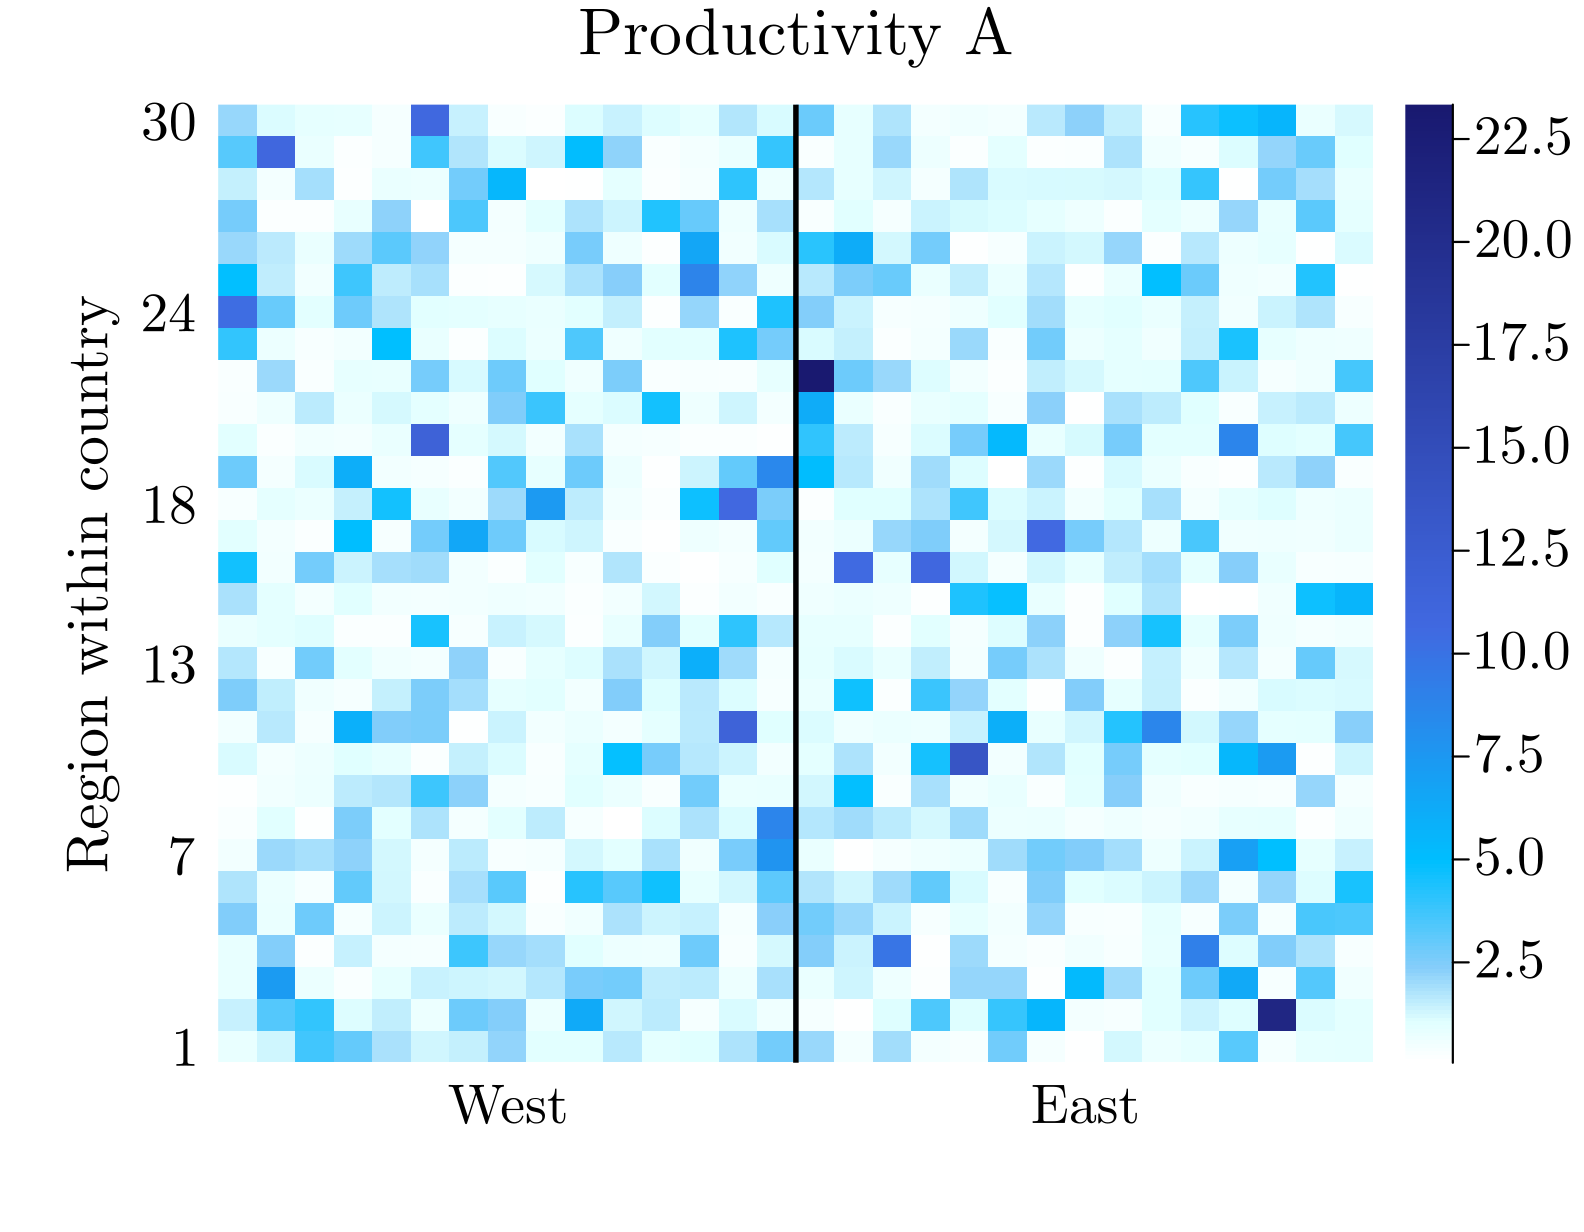
\includegraphics[height=0.62\textheight]
    {worked_example_fundamentals.png}

  \vspace{0.10em}
  \footnotesize
  Only productivity varies across regions:
  \(\operatorname{sd}(\log A_i)=1.00\), with \(A_i\) normalized within each
  country. The benchmark holds \(B_i=1\), \(H_i=100\), and \(F=1\) everywhere,
  with \(\bar L_c=50{,}000\) in each country.

  \vfill
  \hfill\backlink{appInputs}{Back to Inputs}
\end{frame}

\begin{frame}[label=visGeography]{Iceberg Trade Costs}
  \scriptsize
  \begin{columns}[T,onlytextwidth]
    \begin{column}{0.57\textwidth}
      \centering
      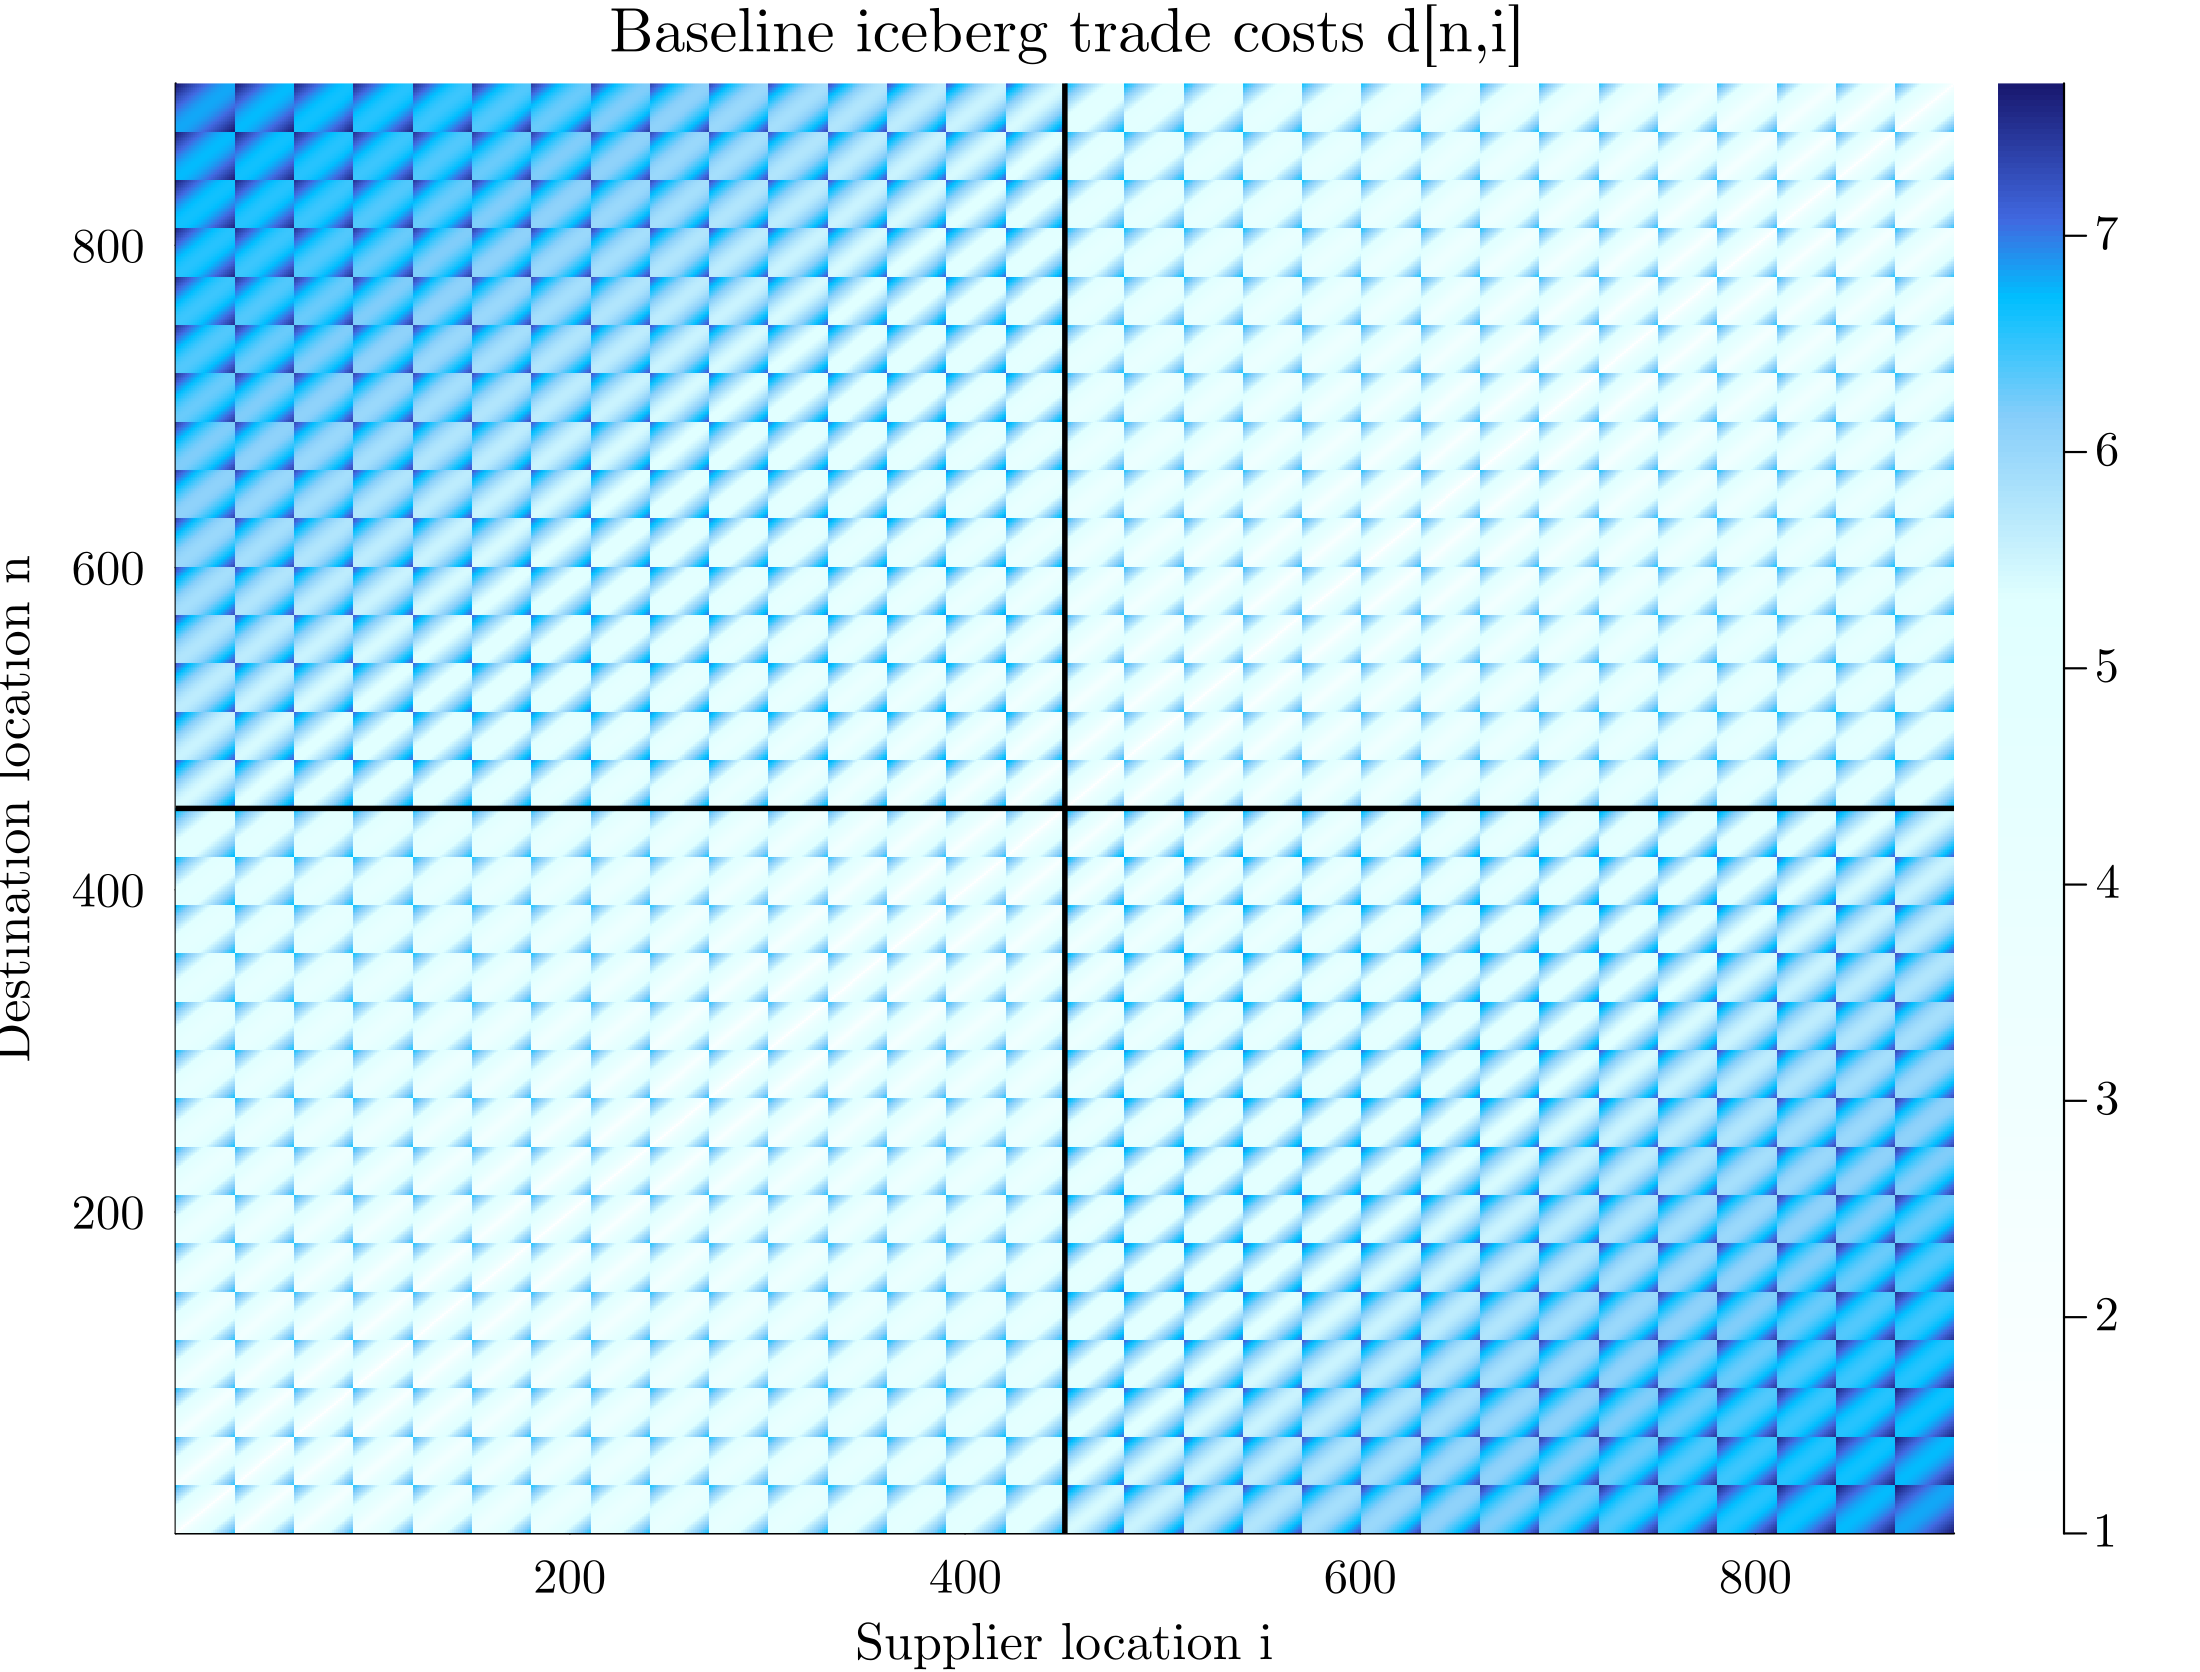
\includegraphics[
        width=\linewidth,
        height=0.50\textheight,
        keepaspectratio
      ]
        {worked_example_trade_costs.png}
    \end{column}
    \begin{column}{0.39\textwidth}
      \B{Direction}
      \begin{itemize}\setlength{\itemsep}{3pt}
        \item \(i\) is the \B{origin}; \(n\) is the \B{destination}.
        \item \(d_{ni}\) is the iceberg cost of shipping a good
          \B{from region \(i\) to region \(n\)}.
      \end{itemize}

      \B{Baseline setting}
      \begin{align*}
        d_{nn}&=1,\\
        d_{ni}^{\mathrm{dom}}
          &=2\,\mathrm{dist}_{ni}^{0.35},\\
        d_{ni}^{\mathrm{int}}
          &=2\times2
            \left(\frac{\mathrm{dist}_{ni}}{6.303}\right)^{0.35}.
      \end{align*}
      The bilateral-liberalization counterfactual sets
      \(\widehat d_{ni}=0.9\) whenever
      \(c(n)\neq c(i)\).
      The internal-liberalization counterfactual sets
      \(\widehat d_{ni}=0.9\) whenever
      \(c(n)=c(i)\) and \(n\neq i\).
    \end{column}
  \end{columns}
  \vfill
  \hfill\backlink{appInputs}{Back to Inputs}
\end{frame}

\begin{frame}[label=visBaseline]{Baseline Equilibrium: Spatial Distribution}
  \centering
  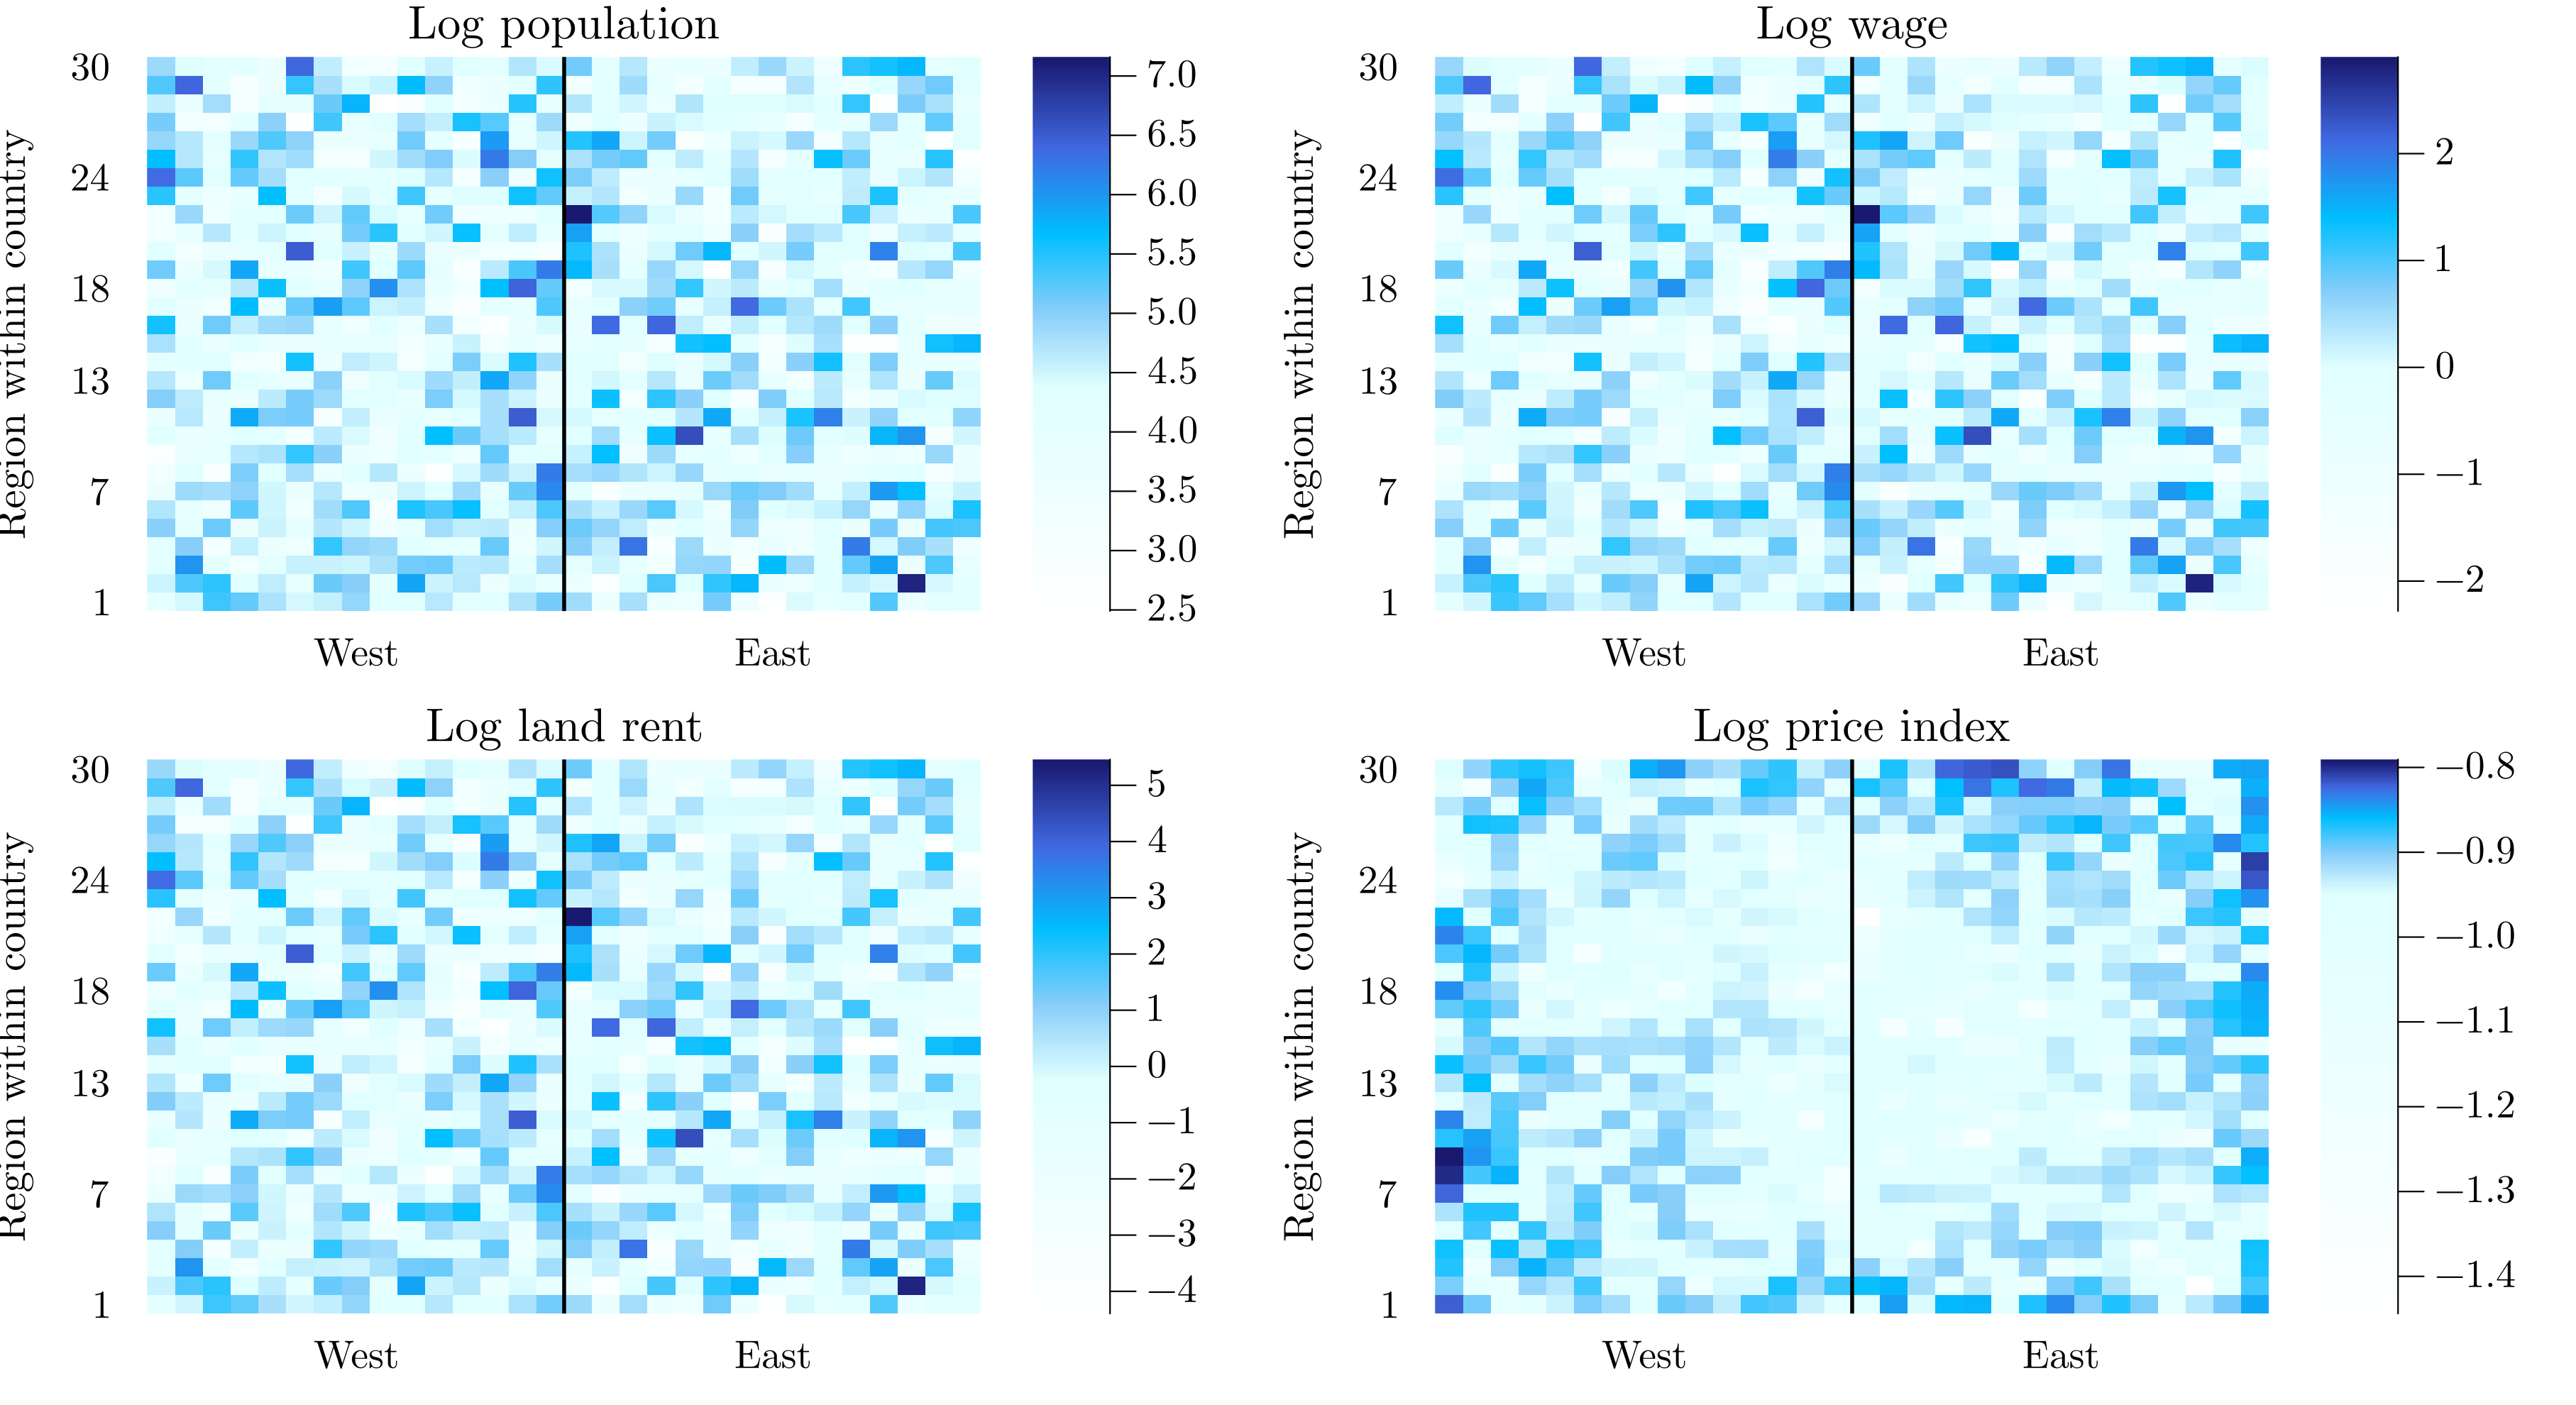
\includegraphics[height=0.73\textheight]
    {worked_example_baseline.png}

  \vspace{0.05em}
  \scriptsize\observablesource

  \vfill
  \hfill\backlink{appInputs}{Back to Inputs}
\end{frame}

\begin{frame}[label=visTradeMatrix]{Visualizing Bilateral Expenditure Shares}
  \centering
  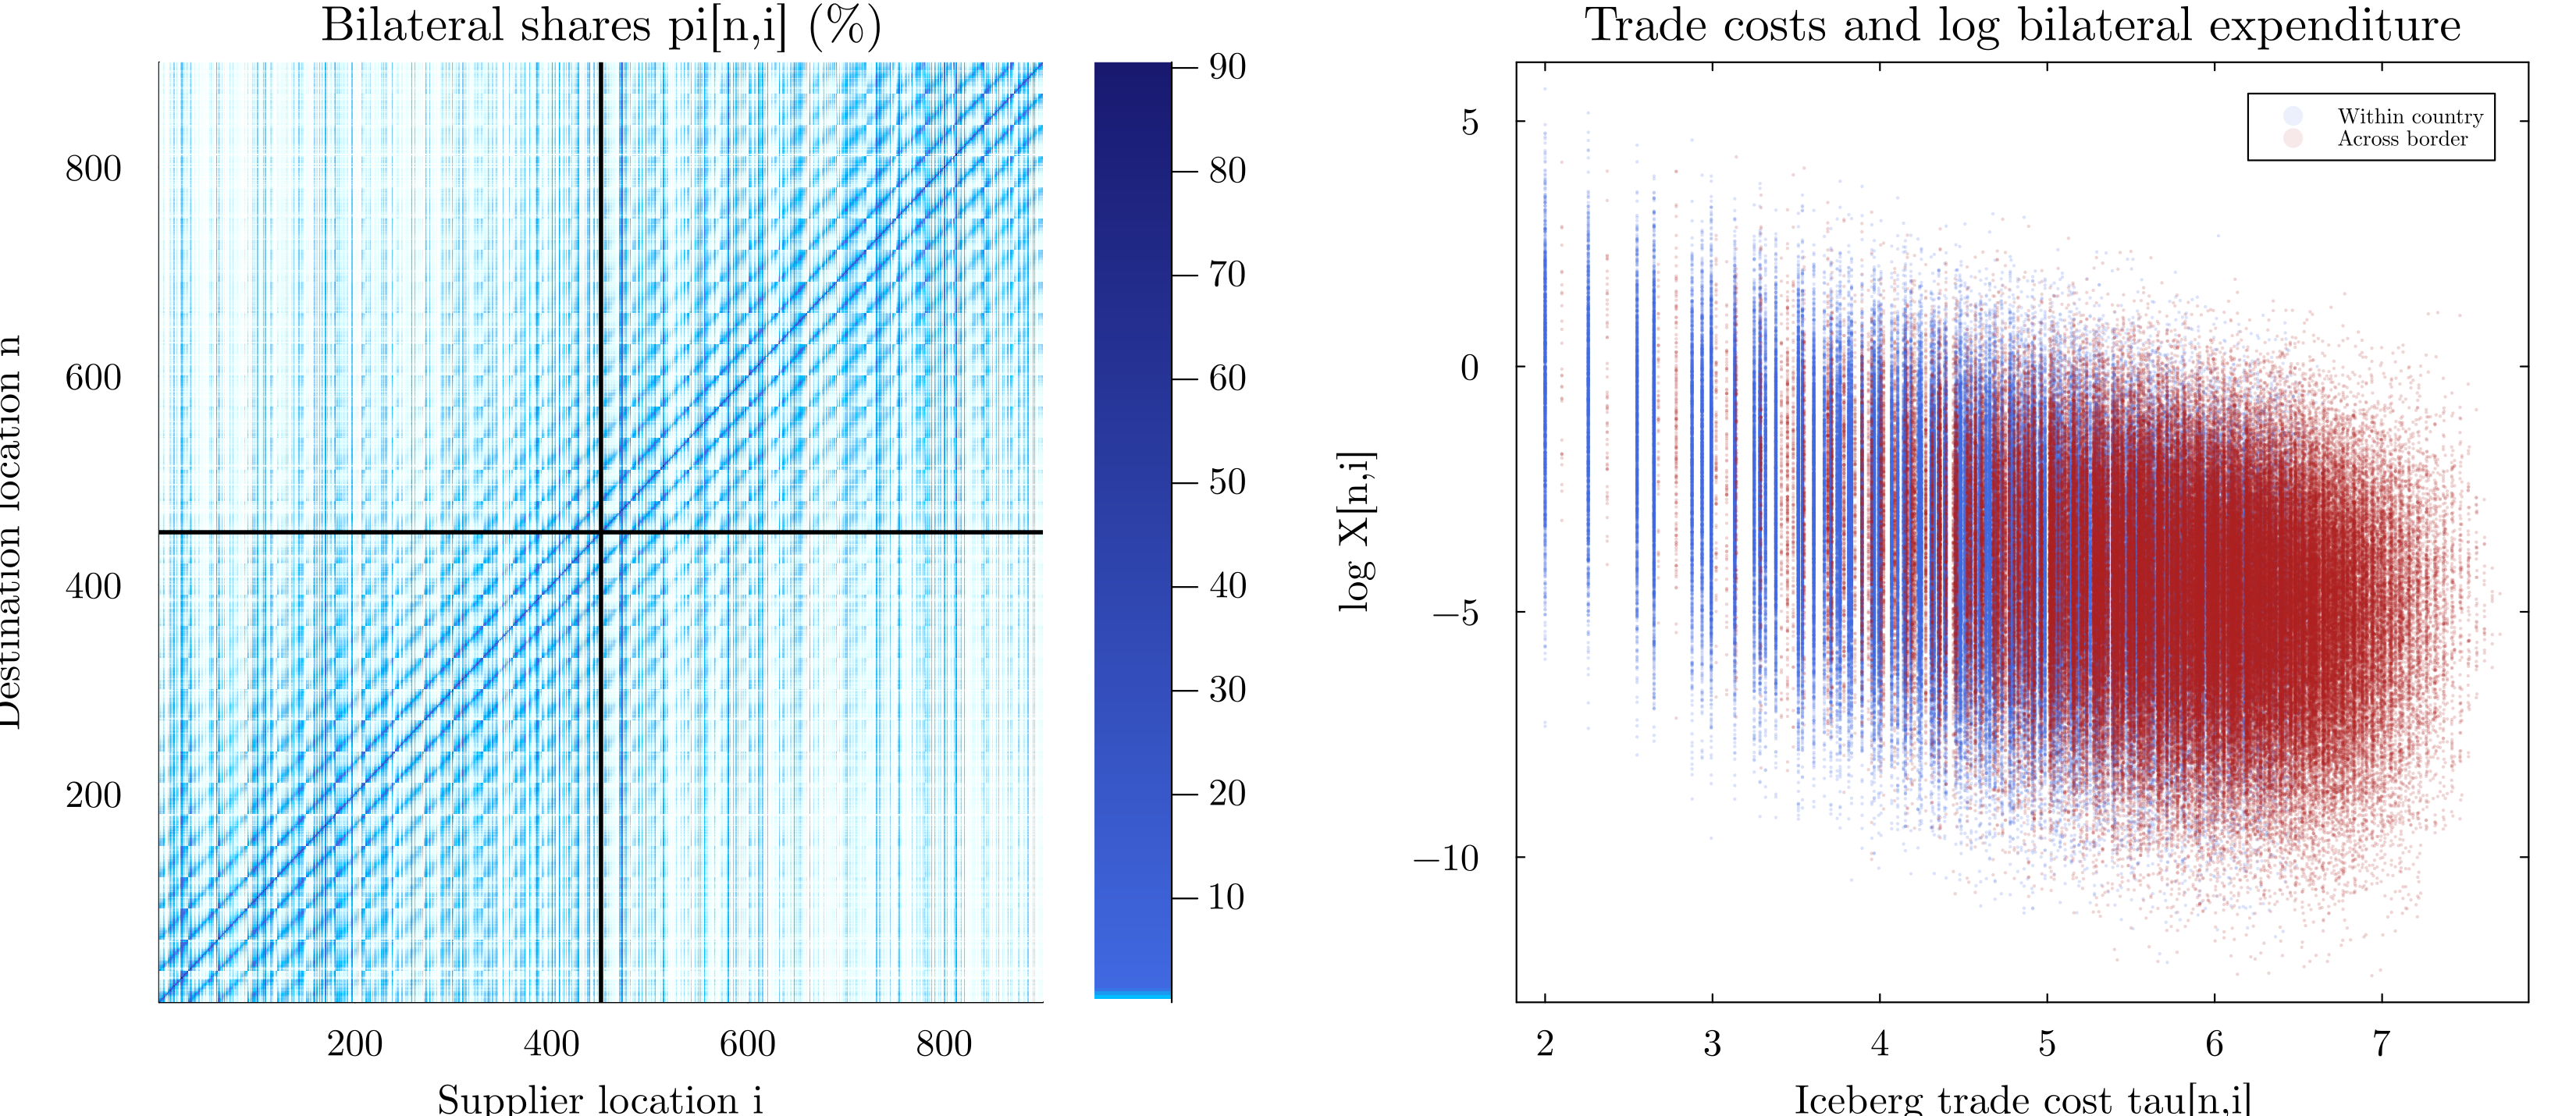
\includegraphics[width=0.91\textwidth]
    {worked_example_trade_matrix.png}

  \scriptsize
  Left: full \(\pi_{ni}\), with destinations by row and suppliers by column.
  Right: \(\tau_{ni}\equiv d_{ni}\) against
  \(\log X_{ni}\), where \(X_{ni}=\pi_{ni}E_n\), for \(n\neq i\).
  The heatmap reports \(\pi_{ni}\) in levels with nonlinear color spacing.

  \hfill\backlink{appInputs}{Back to Inputs}
\end{frame}

\subsection{Derivations}

\begin{frame}[label=appCES]{CES Demand I: Expenditure Minimization}
  For a target \(C_n\), minimize expenditure:
  \[
    \min_{\{c_{ni}(j)\}}
    \sum_i\int_0^{M_i}p_{ni}(j)c_{ni}(j)dj
  \]
  subject to
  \[
    \left[
      \sum_i\int_0^{M_i}
      c_{ni}(j)^{\frac{\sigma-1}{\sigma}}dj
    \right]^{\frac{\sigma}{\sigma-1}}
    \geq C_n.
  \]
  The first-order conditions imply
  \[
    \frac{c_{ni}(j)}{c_{nk}(j')}
    =
    \left[
      \frac{p_{ni}(j)}{p_{nk}(j')}
    \right]^{-\sigma},
    \qquad
    c_{ni}(j)=K_np_{ni}(j)^{-\sigma}.
  \]

  \smallskip
  \hfill\backlink{mainPreferences}{Back to Module 1}
\end{frame}

\begin{frame}{CES Demand II: Price Index and Marshallian Demand}
  Substituting \(c_{ni}(j)=K_np_{ni}(j)^{-\sigma}\) into the budget gives
  \[
    E_n
    =
    K_n\sum_i\int_0^{M_i}p_{ni}(j)^{1-\sigma}dj.
  \]
  The unit-expenditure function is
  \[
    P_n
    =
    \left[
      \sum_i\int_0^{M_i}p_{ni}(j)^{1-\sigma}dj
    \right]^{1/(1-\sigma)}.
  \]
  Therefore
  \[
    K_n=P_n^{\sigma-1}E_n,
    \qquad
      c_{ni}(j)
      =
      p_{ni}(j)^{-\sigma}P_n^{\sigma-1}E_n.
  \]

  \smallskip
  \hfill\backlink{mainPreferences}{Back to Module 1}
\end{frame}

\begin{frame}[label=appProduction]{Markup Pricing and Free Entry}
  \small
  With demand \(q(p)=Kp^{-\sigma}\), a firm's variable profit is
  \[
    \pi(p)=(p-mc)Kp^{-\sigma}.
  \]
  The first-order condition is
  \[
    Kp^{-\sigma}
    -\sigma(p-mc)Kp^{-\sigma-1}=0,
  \]
  giving
  \[
    p=\frac{\sigma}{\sigma-1}mc.
  \]
  The markup implies variable profit equals revenue divided by \(\sigma\).
  Zero profit gives
  \[
    \frac{R_i}{\sigma}=w_iF,
    \qquad
    R_i=\sigma w_iF.
  \]
  Variable cost is \((\sigma-1)R_i/\sigma=(\sigma-1)w_iF\), so aggregate
  labor-market clearing gives
  \[
    L_i=M_i\left[F+(\sigma-1)F\right]
    \quad\Longrightarrow\quad
    M_i=\frac{L_i}{\sigma F}.
  \]

  \smallskip
  \hfill\backlink{mainProduction}{Back to Module 2}
\end{frame}

\begin{frame}[label=appTrade]{Trade Shares: Aggregation and Symmetry}
  \small
  Spending in destination \(n\) on all varieties from origin \(i\) is
  \[
    X_{ni}
    =
    \int_0^{M_i}p_{ni}(j)c_{ni}(j)\,dj.
  \]
  Therefore
  \[
    \pi_{ni}
    \equiv
    \frac{\displaystyle\int_0^{M_i}p_{ni}(j)c_{ni}(j)\,dj}
         {\displaystyle\sum_k\int_0^{M_k}p_{nk}(j)c_{nk}(j)\,dj}.
  \]
  Symmetry across firms within an origin gives
  \[
    \pi_{ni}
    =
    \frac{M_ip_{ni}c_{ni}}
         {\sum_kM_kp_{nk}c_{nk}}.
  \]

  \vfill
  \hfill\hyperlink{appTradeCES}{\textcolor{blue1}{\footnotesize
  CES-demand substitution \(\longrightarrow\)}}
\end{frame}

\begin{frame}[label=appTradeCES]{Trade Shares: Substituting CES Demand}
  \small
  CES demand for a representative variety from origin \(i\) is
  \[
    c_{ni}=p_{ni}^{-\sigma}P_n^{\sigma-1}E_n.
  \]
  Substitution cancels the common terms \(P_n^{\sigma-1}E_n\):
  \[
    \pi_{ni}
    =
    \frac{M_ip_{ni}^{1-\sigma}}
         {\sum_kM_kp_{nk}^{1-\sigma}}.
  \]

  \smallskip
  \hfill\backlink{mainTradeShares}{Back to Module 3}
\end{frame}

\begin{frame}[t,label=appHousingIncome]{Housing, Income, and Indirect Utility}
  \footnotesize
  Let the per-capita housing-rent transfer be
  \[
    t_n\equiv\frac{r_nH_n}{L_n}.
  \]
  The household budget and Cobb--Douglas demands are
  \[
    P_nC_n+r_nh_n=y_n+t_n,
    \qquad
    P_nC_n=\alpha(y_n+t_n),
    \qquad
    r_nh_n=(1-\alpha)(y_n+t_n).
  \]
  Housing-market clearing implies \(H_n=L_nh_n\), so \(t_n=r_nh_n\).
  Therefore
  \[
    P_nC_n=y_n,
    \qquad
    r_nh_n=\frac{1-\alpha}{\alpha}y_n,
    \qquad
    r_n=\frac{1-\alpha}{\alpha}\frac{y_nL_n}{H_n}.
  \]
  The within-location value, up to a common normalization, is
  \[
    V_n
    =\frac{y_n}{P_n^\alpha r_n^{1-\alpha}}.
  \]
  Substituting housing-market clearing gives
  \[
    V_n
    =
    \left(\frac{\alpha}{1-\alpha}\right)^{1-\alpha}
    \frac{y_n^\alpha H_n^{1-\alpha}}
    {P_n^\alpha L_n^{1-\alpha}}.
  \]

  \vfill
  \hfill\backlink{mainMigration}{Back to Module 5}
\end{frame}

\begin{frame}[label=appMigration]{Location Choice: Shares and Expected Welfare}
  \footnotesize
  Let deterministic location utility be
  \[
    v_n=B_nV_n,
    \qquad
    V_n=\frac{y_n}{P_n^\alpha r_n^{1-\alpha}},
  \]
  and let \(z_{no}\) be independent Fr\'echet with
  \[
    \Pr(z_{no}\leq z)=\exp(-z^{-\kappa}).
  \]
  Since the maximum of independent Fr\'echet variables is also Fr\'echet,
  \[
    \Pr\!\left(\max_n\{v_nz_{no}\}\leq u\right)
    =
    \exp\left[-u^{-\kappa}\sum_nv_n^\kappa\right].
  \]
  Therefore
  \[
    \lambda_n
    =
    \frac{v_n^\kappa}{\sum_kv_k^\kappa},
    \qquad
    \E[U_o^*]
    =
    \Gamma\!\left(1-\frac{1}{\kappa}\right)
    \left(\sum_nv_n^\kappa\right)^{1/\kappa}.
  \]

  Substituting the income and housing-market equations from the preceding
  derivation yields the exact migration share on the main slide.

  \smallskip
  \hfill\backlink{mainMigration}{Back to Module 5}
\end{frame}

\begin{frame}[label=appEquilibrium]{Equilibrium Closure: Market Clearing}
  Bilateral expenditure is \(X_{ni}=\pi_{ni}E_n\). Total sales of origin
  \(i\) are therefore
  \[
    R_i=\sum_nX_{ni}=\sum_n\pi_{ni}E_n.
  \]
  With labor as the only factor and zero profits, revenue is paid to labor:
  \[
    R_i=w_iL_i
    \quad\Longrightarrow\quad
    w_iL_i=\sum_n\pi_{ni}E_n.
  \]
  With endogenous population, labor-market clearing supplies local labor:
  \[
    L_i=\bar L\lambda_i.
  \]
  The production block has already converted local labor into the mass of firms;
  that condition need not be repeated here.

  \smallskip
  \hfill\hyperlink{appTradeBalance}{\textcolor{blue1}{\footnotesize
  \(\longrightarrow\) Trade-balance derivation}}
\end{frame}

\begin{frame}[label=appTradeBalance]{Equilibrium Closure: Trade Balance}
  Begin with the trade-balance identity
  \[
    IM_n=EX_n+D_n.
  \]
  Imports and exports are
  \[
    IM_n=\sum_{i\neq n}\pi_{ni}E_n=(1-\pi_{nn})E_n,
    \qquad
    EX_n=\sum_{m\neq n}\pi_{mn}E_m.
  \]
  Goods-market clearing for origin \(n\) implies
  \[
    EX_n=w_nL_n-\pi_{nn}E_n.
  \]
  Substituting both expressions into the original identity gives
  \[
  \begin{aligned}
    (1-\pi_{nn})E_n
      &=w_nL_n-\pi_{nn}E_n+D_n\\
    E_n-w_nL_n
      &=D_n\\
    E_n
      &=w_nL_n+D_n.
  \end{aligned}
  \]
  Across all locations, \(\sum_nD_n=0\).
  \hfill\backlink{mainEquilibrium}{Back to Module 7}
\end{frame}

\begin{frame}{Exact-Hat Algebra: Basic Rules}
  For any variable \(x\),
  \[
    \wh x\equiv\frac{x'}{x}.
  \]
  Products, ratios, and powers satisfy
  \[
    \wh{xy}=\wh x\,\wh y,
    \qquad
    \wh{x/y}=\frac{\wh x}{\wh y},
    \qquad
    \wh{x^a}=(\wh x)^a.
  \]
  Exact-hat algebra divides each counterfactual equilibrium equation by its
  baseline counterpart:
  \begin{itemize}\setlength{\itemsep}{5pt}
    \item unchanged level constants cancel;
    \item baseline expenditure or revenue shares become weights;
    \item the resulting change equations remain exact conditional on the model.
  \end{itemize}
\end{frame}

\begin{frame}[t,label=appHatTrade]{Exact-Hat Derivation: Price Index and Trade Share}
  \scriptsize
  Start from the two price-index equations:
  \[
    P_n^{1-\sigma}
      =\frac{\mu^{1-\sigma}}{\sigma F}
      \sum_iL_i(d_{ni}w_i/A_i)^{1-\sigma},
    \qquad
    P_n'^{\,1-\sigma}
      =\frac{\mu^{1-\sigma}}{\sigma F'}
      \sum_iL_i'(d_{ni}'w_i'/A_i')^{1-\sigma}.
  \]
  Dividing the second by the first and recognizing the baseline trade shares gives
  \[
    \wh P_n^{1-\sigma}
    =\wh F^{-1}\sum_i
      \underbrace{\frac{L_i(d_{ni}w_i/A_i)^{1-\sigma}}
      {\sum_kL_k(d_{nk}w_k/A_k)^{1-\sigma}}}_{\pi_{ni}}
      \wh L_i(\wh d_{ni}\wh w_i/\wh A_i)^{1-\sigma}.
  \]
  For trade shares, divide the counterfactual share by the baseline share:
  \[
    \wh\pi_{ni}
    =\frac{\wh L_i(\wh d_{ni}\wh w_i/\wh A_i)^{1-\sigma}}
      {\sum_k\pi_{nk}\wh L_k
      (\wh d_{nk}\wh w_k/\wh A_k)^{1-\sigma}}.
  \]
  The price-index equation replaces the denominator:
  \[
    \wh\pi_{ni}
    =\frac{\wh F^{-1}\wh L_i
      (\wh d_{ni}\wh w_i/\wh A_i)^{1-\sigma}}
      {\wh P_n^{1-\sigma}}.
  \]

  \vfill
  \hfill\backlink{mainHatSystem}{Back to Exact-Hat System}
\end{frame}

\begin{frame}[t,label=appHatClosure]{Exact-Hat Derivation: Wages and Population}
  \scriptsize
  \setlength{\abovedisplayskip}{2pt}
  \setlength{\belowdisplayskip}{2pt}
  Divide counterfactual goods-market clearing by baseline market clearing:
  \begin{align*}
    \wh w_i\wh L_i
    &=
    \sum_n
    \frac{w_nL_n\pi_{ni}}{w_iL_i}
    \wh\pi_{ni}\wh w_n\wh L_n
    \\[-1pt]
    \Longrightarrow\qquad
    \wh w_i
    &=
    \frac{1}{\wh L_iw_iL_i}
      \sum_n\wh\pi_{ni}\wh w_n\wh L_n(w_nL_n\pi_{ni}).
  \end{align*}

  Under balanced trade, \(y_n=w_n\). After imposing housing-market clearing,
  the indirect-utility hat is
  \[
    \wh V_n
    =
    \frac{\wh w_n^\alpha\wh H_n^{1-\alpha}}
    {\wh P_n^\alpha\wh L_n^{1-\alpha}}.
  \]
  The baseline and counterfactual migration shares are
  \[
    \lambda_n=\frac{(B_nV_n)^\kappa}
      {\sum_k(B_kV_k)^\kappa},
    \qquad
    \lambda_n'=\frac{(B_n'V_n')^\kappa}
      {\sum_k(B_k'V_k')^\kappa}.
  \]
  Dividing and collecting baseline shares gives
  \[
    \wh\lambda_n
    =\frac{(\wh B_n\wh V_n)^\kappa}
      {\sum_k\lambda_k
      (\wh B_k\wh V_k)^\kappa}.
  \]
  Finally, \(L_n=\bar L\lambda_n\) implies
  \(\wh L_n=\wh{\bar L}\,\wh\lambda_n\).

  \vfill
  \hfill\backlink{mainHatSystem}{Back to Exact-Hat System}
\end{frame}

\end{document}
